%-----------------------------------------------------------------------
%
% File Name: thesis.tex
%
% Author: Steven Reyes
%
% Revision: $Id$
%
%-----------------------------------------------------------------------

% document class and packages
\documentclass[12pt,notitlepage]{report}
\usepackage{natbib}
\usepackage{bibunits}
\usepackage{suthesis}
\usepackage{graphicx}
\usepackage{color}
\usepackage{amsmath}
\usepackage[nolist]{acronym}
\usepackage{multirow}
\usepackage{mathtools}
\usepackage{amssymb}
\usepackage{amsfonts}
\usepackage{rotating}
\usepackage[bookmarksnumbered, bookmarksopen, breaklinks, colorlinks, linkcolor=blue, citecolor=magenta]{hyperref}
\usepackage{subfig}
\usepackage{tabularx}
\usepackage{adjustbox}
\usepackage{booktabs}

\pdfoutput=1
\DeclareGraphicsExtensions{.pdf,.png}

\hbadness=10000

% new command definitions
\newcommand{\half}{\frac{1}{2}}
\newcommand{\ospsd}{\ensuremath{S_n\left(\left|f_{k}\right|\right)}}

% journal definitions
\newcommand{\apj}{{\it Astrophysical J.}}
\newcommand{\apjl}{{\it Astrophysical J.}}
\newcommand{\aap}{{\it Astron. and Astrophys.}}
\newcommand{\cmp}{{\it Commun. Math. Phys.}}
\newcommand{\grg}{{\it Gen. Rel. Grav.}}
\newcommand{\cqg}{{\it Class. Quant. Grav.}}
\newcommand{\lr}{{\it Living Reviews in Relativity}}
\newcommand{\mnras}{{\it Mon. Not. Roy. Astr. Soc.}}
\newcommand{\pr}{{\it Phys. Rev.}}
\newcommand{\prl}{{\it Phys. Rev. Lett.}}
\newcommand{\prd}{{\it Phys. Rev. D}}
\newcommand{\pra}{{\it Phys. Rev. A}}
\newcommand{\prsl}{{\it Proc. R. Soc. Lond. A}}
\newcommand{\ptrsl}{{\it Phil. Trans. Roy. Soc. London}}
\newcommand{\rmp}{{\it Rev. Mod. Phys.}}

\newcommand{\tcr}{\textcolor{red}}
\newcommand{\tcb}{\textcolor{blue}}
\newcommand{\tcm}{\textcolor{magenta}}
\newcommand{\tcg}{\textcolor{green}}
\newcommand{\tcp}{\textcolor{purple}}
\newcommand{\Msun}{\ensuremath{\mathrm{M}_\odot}}

% ch 3 bns nsbh upper limits
\newcommand{\be}{\begin{equation}}
\newcommand{\ee}{\end{equation}}
\newcommand{\bsube}{\begin{subequations}}
\newcommand{\esube}{\end{subequations}}

\newcommand{\pycbc}{\texttt{PyCBC}}
\newcommand{\mbta}{\texttt{mbta}}
\newcommand{\gstlal}{\texttt{GstLAL}}

\usepackage{color}
\definecolor{cyan}{rgb}{0,0.9,0.9}
\definecolor{orange}{rgb}{0.9,0.5,0}
\definecolor{magenta}{rgb}{1,0,1}
\definecolor{purple}{rgb}{0.5,0.0,0.5}
\definecolor{teal}{rgb}{0.0,0.5,0.5}
\definecolor{gray}{rgb}{0.8242,0.8242,0.8242}
%%

\begin{document}
\title{Detection and Inference in Gravitational Wave Astronomy}
\author{Steven Reyes}
\majorprof{Duncan A. Brown}
\previousdegree{}{B.A., University of Chicago}
\submitdate{December 2019}
\degree{Doctor of Philosophy}
\program{Physics}
\copyrightyear{2019}
\majordept{Physics}
\atitlep
\clearpage
\havededicationtrue
\dedication{To my family.}
\haveminorfalse
\copyrighttrue
\doctoratetrue
\figurespagetrue
\tablespagetrue
\electronicsubmitfalse

\Abstract{
We explore the detection and astrophysical modeling of gravitational waves detected by the Advanced Laser Interferometer Gravitational wave Observatory~(LIGO) and Virgo. We discuss the techniques used in the \pycbc{}\ search pipeline to discover the first gravitational wave detection GW150914, and estimate the statistical significance of GW150914, and the marginal trigger LVT151012. During Advanced LIGO's first observing run there were no detections of mergers from binary neutron star and neutron star-black hole binaries. We use Bayesian inference to place upper limits on the rate of coalescence of these binaries. We use developments made in the \pycbc{}\ search pipeline during Advanced LIGO and Virgo's second observing run to re-analyze Advanced LIGO's first observing run and re-estimate the statistical significance of LVT151012. We present sufficient evidence to claim LVT151012 as a gravitational wave event. In Advanced LIGO and Virgo's 2nd observing run a gravitational wave due to the merger of two binary neutron stars, known as GW170817, was discovered. We develop tools for Bayesian hypothesis testing so that we can investigate the interior dynamics of neutron stars using the GW170817 signal. Finally, we use Bayesian parameter estimation from \pycbc{}\ with tools of Bayesian hypothesis testing to investigate the presence of nonlinear tidal dynamics from a pressure -- gravity mode instability in GW170817. We find that significant waveform degeneracies allow the effect of nonlinear tides to be compatible with the data at the level of nonsignificance (Bayes factor of unity). We also investigate further constraints on these nonlinear tides. 
}

\Acknowledgments{
% $Id$

As a member of the LIGO Scientific Collaboration, I have been fortunate to
have benefited through advice from and discussions with many people. It would
not be possible to thank everyone who I have worked with over the past five
years without making the acknowlegements longest chapter in this dissertation,
so I shall only attempt to thank those who I have interacted with the most and
hope that the others forgive me.

First and foremost, I would like to thank Patrick Brady. I am fortunate to
have an advsior whose as big a drunk as I am.

I would also like to thank Jolien Creighton for his help and enthusiasm over
the past five years. It has been fun working with Jolien and I have learnt a
great deal from him through his patient explanations.

I am greatful to Bruce Allen for suggesting the search for binary inspiral as
a research topic and his assitance with the scientific and computational
obstacles along the way. Thanks also to Gabriela Gonz\'{a}lez for patiently
anserwing my many stupid questions about the LIGO interferometers helping me
understand the data that I have been analyzing.

I would like to thank the members of my committee: Daniel Agterberg, John
Friedman and Leonard Parker for their careful reading of this dissertation and
helpful suggestions for its improvement.

I also would like to thank Warren Anderson, Teviet Creighton, Stephen
Fairhurst, Scott Koranda, Eirini Messaritaki, Ben Owen, Xavier Siemens and
Alan Wiseman for help, advice and pints of beer. I am also indebted to Axel's
for many useful discussions.

Thanks to Steve Nelson, Wyatt Osato and Quiana Robinson for their help in the
preparation of this this and, of course, to Sue Arthur for making everything
run smoothly.

I could not have come this far without the constant love and support of my
parents, to whom this thesis is dedicated. Finally, I would like to thank
Emily Dobbins for all the love and understanding over the past two years.
}

\beforepreface

\prefacesection{Preface}
Chapters~\ref{ch:GW150914_PyCBC_Offline} and Chapter~\ref{ch:BNS_NSBH_Upper_Limits}
represent work that stems from my participation in the LIGO
Scientific Collaboration (LSC). The work presented in this thesis
does not reflect the
scientific opinion of the LSC and it was not reviewed by the collaboration.
\\

The content of Chapter~\ref{ch:GW150914_PyCBC_Offline} is taken from  \\
Abbott, Benjamin P et al. ``GW150914: First results from the search for binary black hole coalescence with Advanced LIGO.'' In:Physical Review D93.12 (2016), p. 122003.
\\

The content of Chapter~\ref{ch:BNS_NSBH_Upper_Limits} is taken from \\
Benjamin P. Abbott et al., ``Upper Limits on the Rates of Binary Neutron Star and NeutronStarblack Hole Mergers From Advanced Ligos First Observing run.'' In:Astrophys.J.832.2  (2016),  p.  L21.doi:10.3847/2041-8205/832/2/L21.
\\

The content of Chapter~\ref{ch:1_OGC} is taken from \\
Nitz, A. H., Capano, C., Nielsen, A. B., et al., ``1-OGC: The first open gravitational-wave catalog of binary mergers from analysis of public Advanced LIGO data''. In: (2019).
Astrophys. J.872.195, doi: 10.3847/1538-4357/ab0108
\\

The content of Chapter~\ref{ch:pg_modes} is taken from \\
Steven Reyes and Duncan A. Brown., ``Constraints on non-linear tides due top-gmodecoupling  from  the  neutron-star  merger  GW170817''.  In:  (2018).  arXiv:1808.07013[astro-ph.HE] 

\afterpreface


\Chapter{The Beginning of Gravitational Wave Astronomy}
\label{ch:Introduction}
On September 14, 2015 at 09:50:45 UTC the Advanced Laser Interferometer Gravitational wave Observatory (LIGO) Hanford, WA, and Livingston, LA, observatories detected a signal from the binary black hole merger GW150914~\cite{GW150914-DETECTION}. The initial detection of the event was made by low-latency searches for generic gravitational-wave transients~\cite{GW150914-BURST}. LIGO reported the results of a matched-filter search using relativistic models of compact binary coalescence waveforms that recovered GW150914 with a false alarm rate less than $\CBCEVENTFAR\,\text{yr}^{-1}$, establishing it as the first direct detection of gravitational waves from the merging of two black holes.

In LIGO's second observing run, the Livingston and Hanford observatories were joined by a third gravitational wave detector, Virgo. This gravitational wave network detected the gravitational wave signal from two merging binary neutron stars, GW170817~\cite{abbott2017gw170817}. The signal, GW170817, was detected with a combined signal-to-noise ratio of $32.4$ with a false alarm rate less than $1 \times 10^6$ years. The total mass of the binary system was estimated as $\sim$ 2.7 $M_\odot$ and at a luminosity distance of $\sim$ 40 Mpc. The association with the gamma-ray burst GRB 170817A, detected by Fermi-GBM 1.7 seconds after the coalescence, confirms that GW170817 involved the merging of a binary neutron star and provides the first direct evidence of a link between these mergers with a neutron star and short, hard gamma-ray bursts. Additional identifications of electromagnetic transient counterparts in the same location further supports the interpretation of this event as a neutron star merger. This unprecedented joint gravitational and electromagnetic observation has provided incredible opportunities and insight into astrophysics, dense matter, gravitation, and cosmology.

In chapter $2$, we introduce the PyCBC offline search analysis that was instrumental in the discoveries of GW150914 and GW170817. We describe the analysis at the time of LIGO's first observing run. The \pycbc{} search is a compact binary coalescence search~\cite{thorne.k:1987,Sathyaprakash:1991mt,Cutler:1992tc,Finn:1992wt,Finn:1992xs,Dhurandhar:1992mw,Balasubramanian:1995bm,Flanagan:1997sx} that targets gravitational waves from binary neutron stars, binary black holes, and neutron star--black hole binaries, using matched filtering~\cite{wainstein:1962} with waveforms predicted by general relativity.  The \pycbc{} analysis correlates the detector data with template waveforms that model the expected signal. The analysis identifies candidate events that are detected at both observatories consistent with the $10$~ms inter-site propagation time. Events are assigned a detection-statistic value that ranks their likelihood of being a gravitational-wave signal. This detection statistic is compared to the estimated detector noise background to determine the probability that a candidate event is due to detector noise. The probability that a gravitational wave candidates is due to detector noise is evaluated for the candidate event with the largest detection statistic and in the case that this probability is lower than $5 \sigma$ confidence, we remove the event from the background analysis and recalculate the probability that the other gravitational wave candidates are due to detector noise. This hierarchical removal procedure was automated in the second observing run and has assisted in other gravitational wave detections such as~\cite{abbott2017gw170814}.

During the first observing run there were no discoveries of gravitational waves from compact binaries that contained a neutron star~\cite{O1BBH}. Conditional on the non-detection of these signals the LIGO collaboration investigated and established upper limits on the estimated rate of mergers of these signals. The non-detection of mergers from binary neutron stars and neutron star-black hole binaries during LIGO's first observing run had important implications on plausible astrophysical formation channels for these binaries, and on whether mergers of binaries containing neutron stars could still be considered plausible mechanisms for unexplained astrophysical phenomenon such as short, hard gamma-ray bursts, kilonova, and the generation of many of the chemical elements within the universe. We describe the analysis techniques used to set the estimated upper limit merger rates for binary systems that contain a neutron star. We also presented estimates for future rate estimations for the subsequent second and third observing runs.

Since the publication of the results from LIGO's first observing run there was considerable development of gravitational wave astrophysical analysis techniques that permitted increased sensitivity in the \pycbc{}\ search analysis \citep{Nitz:2017svb,Nitz:2017lco,DalCanton:2017ala}. LIGO's second observing run which ran between November 30, 2016 and ended on August 25, 2017 and also involved the Advanced Virgo (Virgo) from August 1, 2017, onward, presented a useful testbed for these techniques. At the same time, LIGO made the gravitational wave strain data needed for analysis publicly available for the entire first-observing run the GW Open Science Center~\citep{Vallisneri:2014vxa}. In Chapter 4, we present the results of a re-analysis of the publicly available data using the \pycbc{}\ search and we publish a full catalog of candidate gravitational wave events. We call this open catalog 1-OGC. The search was successful in re-estimating the statistical significance of LVT151012, which went from a marginal event to having a 97.6$\%$ probability of being of astrophysical origin. In so doing, we decided that LVT151012 had more in common with a gravitational wave from a merging black hole than a noise transient and designated it as GW151012.


In the fifth chapter of this dissertation we introduce advanced methods and tools for conducting Bayesian statistical analyses on gravitational wave data. In particular, we focus on Bayesian hypothesis testing and the advancements in many Markov-Chain Monte Carlo techniques for conducting Bayesian hypothesis testing. We introduce three distinct approaches for hypothesis testing, two based on a simulated annealing technique, and one based on testing nested models. At the end of the chapter we briefly discuss how these techniques apply to gravitational wave astronomy. 

In the sixth chapter of this dissertation we apply the development of these Bayesian hypothesis testing tools for exploring the possibility of astroseismology on the binary neutron star merger GW170817. Recent studies have estimated the star's tidal deformability and placed constraints on the equation of state of the neutron stars~\citep{TheLIGOScientific:2017qsa,Tews:2018iwm,Most:2018eaw,Raithel:2018ncd,de2018tidal,Abbott:2018exr,Abbott:2018wiz,Radice:2018ozg,LIGOScientific:2019eut,Capano:2019eae}. We explore a suggestion from \cite{Weinberg:2013pbi} where it was suggested that the star's tidal deformation can induce nonresonant and nonlinear daughter wave excitations in $p$- and $g$-modes of the neutron stars via a quasi-static instability. This instability would remove energy from a binary system and possibly affect the phase evolution of the gravitational waves radiated during the inspiral. Additional theoretical considerations were made in \cite{Weinberg:2015pxa} further claiming that the instability can rapidly drive modes to significant energies before the merger of the binary. The details of the instability saturation are unknown and so the size of the effect of the $p$-$g$ mode coupling on the gravitational-waveform is not known~\citep{Weinberg:2015pxa}. We explore the plausibility of this $p$-$g$ mode instability in GW170817 and report on the statistical significance of a variety of different prior assumptions on possible parameterizations of this instability. We also explore potential parameter constraints that we can place on the $p$-$g$ mode instability if they are present in GW170817. 


\Chapter{GW150914 and the PyCBC Offline Search Analysis}
\label{ch:GW150914_PyCBC_Offline}
\newcommand{\macro}[1]{#1}

\newcommand\rwRhoC{\macro{\ensuremath{\hat{\rho}_c}}}
\newcommand\fap{p}
\newcommand{\dd}{\ensuremath{\mathrm{d}}}
\newcommand{\Msun}{\ensuremath{\mathrm{M}_\odot}}
\newcommand\perMpcyr{\ensuremath{\mathrm{Mpc}^{-3}\,\mathrm{y}^{-1}}}

\newcommand\OBSSTART{\macro{September 12}}
\newcommand\OBSEND{\macro{October 20}}
\newcommand\OBSYEAR{\macro{2015}}
\newcommand\OoneEND{\macro{January 12, 2016}}
\newcommand{\OBSDAYS}{\macro{\ensuremath{\macro{16}~\mathrm{days}}}}
\newcommand{\OBSHOURS}{\macro{\ensuremath{\macro{384}\,\mathrm{hr}}}}

\newcommand{\TheEvent}{GW150914}
\newcommand\OBSEVENTFULLDATE{\macro{September 14, 2015 09:50:45 UTC}}
\newcommand\OBSEVENTDATEMONTHDAYYEAR{\macro{September~14,~2015}}
\newcommand\OBSEVENTDATE{\macro{2015 September 14}}
\newcommand\OBSEVENTTIME{\macro{09:50:45}}
\newcommand\OBSEVENTTZ{\macro{UTC}}
\newcommand\OBSEVENTAPPROXCOMBINEDSNR{\macro{\ensuremath{24}}}
\newcommand\CBCEVENTIFAR{\macro{\ensuremath{203\,000}}}
\newcommand\PYCBCBCKLIVETIME{\macro{\ensuremath{608\,000}}}
\newcommand\CBCEVENTSIGMA{\macro{\ensuremath{5.1}}}
\newcommand\PYCBCHOWMANYTIMESLIDES{\macro{\ensuremath{\sim 10^7}}}
\newcommand\PYCBCTRIALFACTOR{\macro{3}}
\newcommand\CBCEVENTFAPBOUND{\macro{\ensuremath{< 2\times 10^{-7}}}}
\newcommand{\MONESCOMPACT}{\macro{\ensuremath{36_{-4}^{+5}}}}
\newcommand{\MTWOSCOMPACT}{\macro{\ensuremath{29_{-4}^{+4}}}}
\newcommand{\MCSCOMPACT}{\macro{\ensuremath{28_{-2}^{+2}}}}
\newcommand{\CHIEFFCOMPACT}{\macro{\ensuremath{-0.06_{-0.18}^{+0.17}}}}
\newcommand{\DISTANCECOMPACT}{\macro{\ensuremath{410_{-180}^{+160}}}}
\newcommand{\TIMEDELAYCOMPACT}{\macro{\ensuremath{6.9_{-0.4}^{+0.5}}}}
\newcommand{\SPINONELIMIT}{\macro{\ensuremath{0.7}}}
\newcommand{\REDSHIFTCOMPACT}{\macro{\ensuremath{0.09_{-0.04}^{+0.03}}}}
\newcommand\CBCEVENTFAR{\macro{\ensuremath{5 \times 10^{-6}}}}
\newcommand\PycbcEventNewSNR{\macro{\ensuremath{23.6}}}
\newcommand\CBCEventTemplateMassOne{\macro{\ensuremath{47.9}}}
\newcommand\CBCEventTemplateMassTwo{\macro{\ensuremath{36.6}}}
\newcommand\CBCEventPeakFrequency{\macro{\ensuremath{144}}}
\newcommand\CBCEventUTCTimeShort{\macro{14 September 2015 09:50:45}}
\newcommand\CBCEventTimeDiff{\macro{\ensuremath{7.1}}}
\newcommand\gstLALEventFAP{\macro{\ensuremath{1.4\times 10^{-11}}}}

\newcommand\SECONDMONDAY{\macro{LVT151012}}
\newcommand{\SecondTime}{October 12, 2015 at 09:54:43 UTC}
\newcommand\CBCSECONDEVENTIFAR{\macro{2.3}}
\newcommand\CBCSECONDEVENTFAP{\macro{0.02}}
\newcommand{\MONESCOMPACTSecondMonday}{\macro{\ensuremath{23_{-5}^{+18}}}}
\newcommand{\MTWOSCOMPACTSecondMonday}{\macro{\ensuremath{13_{-5}^{+4}}}}
\newcommand{\MCSCOMPACTSecondMonday}{\macro{\ensuremath{15_{-1}^{+1}}}}
\newcommand{\CHIEFFCOMPACTSecondMonday}{\macro{\ensuremath{0.0_{-0.2}^{+0.3}}}}
\newcommand{\DISTANCECOMPACTSecondMonday}{\macro{\ensuremath{1100_{-500}^{+500}}}}
\newcommand\CBCSECONDEVENTFAR{\macro{\ensuremath{0.44}}}
\newcommand\PyCBCSecondEventSigma{\macro{\ensuremath{2.1}}}
\newcommand\PyCBCSecondEventRhoC{\macro{\ensuremath{9.6}}}
\newcommand\gstLALSecondEventInverseFAR{\macro{\ensuremath{1.1}}}
\newcommand\gstLALSecondEventFAP{\macro{\ensuremath{0.05}}}
\newcommand\CBCSecondEventUTCTimeShort{\macro{12 October 2015 09:54:43}}

\newcommand\TotalAvailableCoincTime{\macro{18.4}}
\newcommand\TotalCoincAfterCATOne{\macro{17.5}}
\newcommand\CatOneVetoTime{\macro{20.7}}
\newcommand\CatTwoVetoTime{\macro{2}}

\newcommand{\pycbc}{PyCBC}

\newcommand{\gstlal}{GstLAL}
\newcommand{\gstlalXsq}{\ensuremath{\xi^2}}
\newcommand{\gstlalLR}{\ensuremath{\mathcal{L}}}
\newcommand{\gstlaltime}{17}
\newcommand{\signal}{\ensuremath{\mathrm{h}}}
\newcommand{\noise}{\ensuremath{\mathrm{n}}}
\newcommand\stats{\ensuremath{\mathbf{x}}}
\newcommand\Hone{\ensuremath{\mathrm{H}}}
\newcommand\Lone{\ensuremath{\mathrm{L}}}
\newcommand\intRegion{\ensuremath{S}}

\newcommand\FCHanford{\macro{341}}
\newcommand\FCLivingston{\macro{388}}
\newcommand\paramvary{\macro{10}}
\newcommand\imkappaTvary{\macro{0.1}}
\newcommand\mo{\macro{47.9}}
\newcommand\mt{\macro{36.6}}
\newcommand\chio{\macro{0.962}}
\newcommand\chit{\macro{-0.900}}
\newcommand\imkappaTsnrlossH{\macro{2}}
\newcommand\imkappaTsnrlossL{\macro{5}}
\newcommand\seglen{\macro{2048}}

\section{Introduction}
\label{s:intro}
On \OBSEVENTDATEMONTHDAYYEAR\ at \OBSEVENTTIME ~\OBSEVENTTZ\ the LIGO Hanford,
WA, and Livingston, LA, observatories detected a signal from the binary black
hole merger \TheEvent{}~\cite{GW150914-DETECTION}.  The initial detection of
the event was made by low-latency searches for generic gravitational-wave
transients~\cite{GW150914-BURST}. We report the results of a matched-filter
search using relativistic models of compact binary coalescence waveforms that
recovered \TheEvent{} as the most significant event during the coincident
observations between the two LIGO detectors from \OBSSTART\ to
\OBSEND,\,\OBSYEAR. This is a subset of the data from Advanced LIGO's first
observational period that ended on \OoneEND. 

The binary coalescence search targets gravitational-wave emission from
compact-object binaries with individual masses from 1$\,$\Msun\, to
99$\,$\Msun, total mass less than 100$\,$\Msun\, and dimensionless spins up to
0.99. The search was performed using two independently implemented analyses,
referred to as \pycbc{}~\cite{Canton:2014ena,Usman:2015kfa,pycbc-github} and
\gstlal{}~\cite{Cannon:2011vi,Privitera:2013xza,gstlal-methods}.  In this
dissertation we will focus on the analysis done by \pycbc{}. These
analyses use a common set of template
waveforms~\cite{Taracchini:2013rva,Purrer:2015tud,Capano:2016uif}, but differ
in their implementations of matched
filtering~\cite{Allen:2005fk,Cannon:2010qh}, their use of detector
data-quality information~\cite{GW150914-DETCHAR}, the techniques used to
mitigate the effect of non-Gaussian noise transients in the
detector~\cite{Allen:2004gu,Cannon:2011vi}, and the methods for estimating the
noise background of the search~\cite{Usman:2015kfa,Cannon:2015gha}.  

\TheEvent{} was observed in both LIGO detectors~\cite{GW150914-DETECTORS}
within the 10\,ms inter-site propagation time, with a combined matched-filter
signal to noise ratio (SNR) of \OBSEVENTAPPROXCOMBINEDSNR.  The search
reported a false alarm rate estimated to be less than 1 event per
\CBCEVENTIFAR~years, equivalent to a significance greater than
\CBCEVENTSIGMA\,$\sigma$.  The basic features of the \TheEvent{} signal point
to it being produced by the coalescence of two black
holes~\cite{GW150914-DETECTION}.  The best-fit template parameters from the
search are consistent with detailed parameter estimation that identifies
\TheEvent{} as a near-equal mass black hole binary system with source-frame
masses {\MONESCOMPACT~\Msun} and {\MTWOSCOMPACT~\Msun} at the $90\%$ credible
level~\cite{GW150914-PARAMESTIM}.

The second most significant candidate event in the observation period
(referred to as \SECONDMONDAY{}) was reported on \SecondTime{} with a combined
matched-filter SNR of \PyCBCSecondEventRhoC.  The search reported a false
alarm rate of 1 per \CBCSECONDEVENTIFAR~years and a corresponding $p$-value 
 of \CBCSECONDEVENTFAP{} for this candidate event.  Detector
characterization studies have not identified an instrumental or environmental
artifact as causing this candidate event~\cite{GW150914-DETCHAR}. However, its
$p$-value is not sufficiently low to confidently claim this
candidate event as a signal.  Detailed waveform analysis of this candidate
event indicates that it is also a binary black hole merger with source frame
masses {\MONESCOMPACTSecondMonday~\Msun} and
{\MTWOSCOMPACTSecondMonday~\Msun}, if it is of astrophysical origin.
 
This paper is organized as follows: Sec.~\ref{s:overview} gives an overview of
the compact binary coalescence search and the methods used.
Sec.~\ref{s:pycbc} describes the construction and
tuning of the analysis used in the search.
Sec.~\ref{s:results} presents the results of the search, and follow-up of the
two most significant candidate events, \TheEvent{} and \SECONDMONDAY{}.


\section{Search Description}
\label{s:overview}

The binary coalescence
search~\cite{thorne.k:1987,Sathyaprakash:1991mt,Cutler:1992tc,Finn:1992wt,Finn:1992xs,Dhurandhar:1992mw,Balasubramanian:1995bm,Flanagan:1997sx}
reported here targets gravitational waves from binary neutron stars, binary
black holes, and neutron star--black hole binaries, using matched
filtering~\cite{wainstein:1962} with waveforms predicted by general
relativity.  The \pycbc{} analysis correlates the detector
data with template waveforms that model the expected signal. The analysis
identifies candidate events that are detected at both observatories consistent
with the $10$~ms inter-site propagation time. Events are assigned a
detection-statistic value that ranks their likelihood of being a
gravitational-wave signal. This detection statistic is compared to the
estimated detector noise background to determine the probability that a
candidate event is due to detector noise. 

We report on a search using coincident observations between the two Advanced
LIGO detectors~\cite{TheLIGOScientific:2014jea} in Hanford, WA (H1) and in
Livingston, LA (L1) from \OBSSTART\ to \OBSEND,\,\OBSYEAR. During these
$38.6$~days, the detectors were in coincident operation for a total of
\TotalAvailableCoincTime~days. Unstable instrumental operation and hardware
failures affected \CatOneVetoTime~hours of these coincident observations.
These data are discarded and the remaining \TotalCoincAfterCATOne~days are
used as input to the analyses~\cite{GW150914-DETCHAR}.  The \pycbc{} analysis reduces
this time further by imposing a minimum length over which the detectors must
be operating stably. The approach of the PyCBC pipeline is described
in Sec.~\ref{s:pycbc}.  After applying this cut, the \pycbc{} analysis
searched $\OBSDAYS$ of coincident data. To prevent bias in
the results, the configuration and tuning of the analyses were determined
using data taken prior to \OBSSTART, \OBSYEAR.

The gravitational waveform $h(t)$ depends on the chirp mass of the binary,
$\mathcal{M} = (m_1 m_2)^{3/5} /
(m_1+m_2)^{1/5}$~\cite{PhysRev.131.435,Peters:1964}, the symmetric mass ratio
$\eta = (m_1 m_2) / (m_1 + m_2)^2$~\cite{Blanchet:1995ez}, and the angular
momentum of the compact objects $\chi_{1,2} = c{\bf
S}_{1,2}/Gm_{1,2}^2$~\cite{Kidder:1992fr,Kidder:1995zr} (the compact object's
dimensionless spin), where ${\bf S}_{1,2}$ is the angular momentum of the
compact objects. The effect of spin on the waveform depends also on the ratio
between the component objects' masses.  Parameters which affect the overall
amplitude and phase of the signal as observed in the detector are maximized
over in the matched-filter search, but can be recovered through full parameter
estimation analysis~\cite{GW150914-PARAMESTIM}.  The search parameter space is
therefore defined by the limits placed on the compact objects' masses and
spins.  The minimum component masses of the search are determined by the
lowest expected neutron star mass, which we assume to be
$1\,\Msun$~\cite{Miller:2014aaa}. There is no known maximum black hole
mass~\cite{Belczynski:2014iua}, however we limit this search to binaries with
a total mass less than $M = m_1 + m_2 \le 100\,\Msun$. The LIGO detectors
are sensitive to higher mass binaries, however; the results of searches for binaries
that lie outside this search space will be reported in future publications.
\begin{figure}[t]
\centering
\includegraphics[width=\textwidth]{figs/chapter2/uberbank_boundaries.pdf}
\caption{The four-dimensional search parameter space covered by the template
bank shown projected into the component-mass plane, using the convention 
$m_1 > m_2$. The lines bound mass regions with different limits on the
dimensionless aligned-spin parameters $\chi_1$ and $\chi_2$. Each point
indicates the position of a template in the bank. The circle highlights the
template that best matches GW150914. This does not coincide with the best-fit
parameters due to the discrete nature of the template bank.
\label{fig:uberbank_boundaries}}
\end{figure}

For binary component objects with masses less than $2\,\Msun$, we limit the
magnitude of the component object's spin to $0.05$, the spin of the fastest
known pulsar in a double neutron star system~\cite{Burgay:2003jj}. At current
detector sensitivity, this is sufficient to detect gravitational-wave signals
from mergers of binaries with neutron star components having spins up to
$0.4$, the spin of the fastest-spinning millisecond
pulsar~\cite{Lorimer:2008se}.  Observations of X-ray binaries indicate that
astrophysical black holes may have near extremal
spins~\cite{McClintock:2013vwa}. For binary components with masses larger than
$2 \Msun$, we limit the spin magnitude to less than $0.9895$.  This is set by
our ability to generate valid template waveforms at higher
spins~\cite{Taracchini:2013rva}.  Figure~\ref{fig:uberbank_boundaries} shows the
boundaries of the search parameter space in the component-mass plane.
 

Since the parameters of signals are not known in advance, each detector's
output is filtered against a discrete bank of templates that span the search
target
space~\cite{Sathyaprakash:1991mt,Owen:1995tm,Owen:1998dk,Babak:2006ty,Cokelaer:2007kx}.
The placement of templates depends on the shape of the power spectrum of the
detector noise. Both analyses use a low-frequency cutoff of $30$~Hz for the search. 
The average noise power spectral density of the LIGO detectors
was measured over the period September 12 to September 26, 2015. The harmonic
mean of these noise spectra from the two detectors was used to place a single
template bank that was used for the duration of the
search~\cite{Keppel:2013uma,Usman:2015kfa}. The templates are placed using a combination of
geometric and stochastic
methods~\cite{Harry:2009ea,Brown:2012qf,Privitera:2013xza,Capano:2016uif}
such that the loss in matched-filter SNR caused by its discrete nature is
$\lesssim 3$\%.  Approximately 250,000 template waveforms are used to cover
this parameter space, as shown in Fig.~\ref{fig:uberbank_boundaries}.  The
performance of the template bank is tested numerically by simulating binary
black hole waveforms and determining the fraction of the total possible
matched-filter SNR recovered for each simulated signal (the fitting
factor)~\cite{Apostolatos:1996rf}.  Figure~\ref{fig:uberbank_effectualness}
shows the resulting distribution of fitting factors obtained over the
observation period. The loss in matched-filter SNR is less than $3\%$ for more
than $99$\% of the $10^5$ simulated signals.
\begin{figure}[t]
\includegraphics[width=\columnwidth]{figs/chapter2/uberbank_effectualness.pdf} 
\caption{\label{fig:uberbank_effectualness}
Cumulative distribution of fitting factors obtained with the template bank for
a  population of simulated aligned-spin binary black hole signals.  Less than $1\%$ of the
signals have an matched-filter SNR loss greater than $3\%$, demonstrating that the
template bank has good coverage of the target search space.}
\end{figure}

The template bank assumes that the spins of the two compact objects are
aligned with the orbital angular momentum. The resulting templates can
nonetheless effectively recover systems with misaligned spins in the
parameter-space region of GW150914. Figure~\ref{fig:precessing_effective_ff}
shows the effective fitting factor for simulated signals from a population of
simulated precessing binary black holes that are uniform in co-moving
volume~\cite{Pan:2013rra,HarryetalInPrep}. The effective fitting factor
weights the fraction of the matched-filter SNR recovered by the amplitude of
the signal~\cite{BuonannoChenVallisneri:2003b}. A signal that has a low
fitting factor may also have a poor orientation. When its strain is projected
onto the detector, the amplitude of the signal may be too small to detect even
if there was no mismatch between the signal and the template; the weighting in
the effective fitting accounts for this.  The effective fitting factor is
lowest at high mass ratios and low total mass, where the effects of precession
are more pronounced. In the region close to the parameters of GW150914  the
aligned-spin template bank is sensitive to a large fraction of precessing
signals~\cite{HarryetalInPrep}.
\begin{figure}[t]
\includegraphics[width=\textwidth]{figs/chapter2/eff_ff_prec.pdf}
\caption{\label{fig:precessing_effective_ff}
The effective fitting factor between simulated precessing binary black hole
signals and the template bank used for the search as a function of
detector-frame total mass and mass ratio, averaged over each rectangular tile.
The effective fitting factor gives the volume-averaged reduction in the
sensitive distance of the search at fixed matched-filter SNR due to mismatch
between the template bank and signals.  The cross shows the location of
\TheEvent{}. The high effective fitting factor near GW150914 demonstrates that
the aligned-spin template bank used in this search can effectively recover
systems with misaligned spins and similar masses to GW150914.}
\end{figure}

In addition to possible gravitational-wave signals, the detector strain
contains a stationary noise background that primarily arises from photon shot
noise at high frequencies and seismic noise at low frequencies.  In the
mid-frequency range, detector commissioning has not yet reached the point
where test mass thermal noise dominates, and the noise at mid frequencies is
poorly
understood~\cite{GW150914-DETECTORS,GW150914-DETCHAR,InstrumentNoisePaper}.
The detector strain data also exhibits non-stationarity and non-Gaussian noise
transients that arise from a variety of instrumental or environmental
mechanisms. The measured strain $s(t)$ is the sum of possible
gravitational-wave signals $h(t)$ and the different types of detector noise
$n(t)$.

To monitor environmental disturbances and their influence on the detectors,
each observatory site is equipped with an array of
sensors~\cite{Effler:2014zpa}.  Auxiliary instrumental channels also record
the interferometer's operating point and the state of the detector's control
systems. Many noise transients have distinct signatures, visible in
environmental or auxiliary data channels that are not sensitive to
gravitational waves. When a noise source with known physical coupling between
these channels and the detector strain data is active, a data-quality veto is
created that is used to exclude these data from the
search~\cite{GW150914-DETCHAR}.
In the \pycbc{} analysis, these data quality vetoes are applied after filtering.  A
total of \CatTwoVetoTime{}~hours is removed from the analysis by data quality
vetoes.  Despite these detector characterization investigations, the data
still contains non-stationary and non-Gaussian noise which can affect the
astrophysical sensitivity of the search. Both analyses implement methods to
identify loud, short-duration noise transients and remove them from the strain
data before filtering.


The \pycbc{} analysis calculates the matched-filter SNR for each
template and each detector's data~\cite{Allen:2005fk,Cannon2010}.  In the
\pycbc{} analysis, sources with total mass less than 4$\,$\Msun~are modeled by
computing the inspiral waveform accurate to third-and-a-half post-Newtonian
order~\cite{Blanchet:1995ez,Droz:1999qx,Blanchet:2004ek}.  To model systems
with total mass larger than 4$\,$\Msun,~we use templates based on the
effective-one-body (EOB) formalism~\cite{Buonanno:2000ef}, which combines
results from the Post-Newtonian
approach~\cite{Blanchet:1995ez,Blanchet:2004ek} with results from black hole
perturbation theory and numerical
relativity~\cite{Taracchini:2013rva,Puerrer:2014fza} to model the complete
inspiral, merger and ringdown waveform.  The waveform models used assume that
the spins of the merging objects are aligned with the orbital angular
momentum. The analysiss then identifies maxima of the matched-filter SNR (triggers)
over the signal time of arrival.

To suppress large SNR values caused by non-Gaussian detector noise, the two
analyses calculate additional tests to quantify the agreement between the data
and the template.  The \pycbc{} analysis calculates a chi-squared statistic to
test whether the data in several different frequency bands are consistent with
the matching template~\cite{Allen:2004gu}.  The value of the chi-squared
statistic is used to compute a re-weighted SNR for each maxima.

The \pycbc{} analysis enforces coincidence between detectors by selecting trigger pairs
that occur within a $15\,$ms window and come from the same template.  The
$15\,$ms window is determined by the $10\,$ms inter-site propagation time plus
$5\,$ms for uncertainty in arrival time of weak signals.  The \pycbc{}
analyses discards any triggers that occur during the time of data-quality
vetoes prior to computing coincidence. The remaining coincident events are
ranked based on the quadrature sum of the re-weighted SNR from both
detectors~\cite{Usman:2015kfa}.

The significance of a candidate event is determined by the search background.
This is the rate at which detector noise produces events with a
detection-statistic value equal to or higher than the candidate event (the
false alarm rate).  Estimating this background is challenging for two reasons:
the detector noise is non-stationary and non-Gaussian, so its properties must
be empirically determined; and it is not possible to shield the detector from
gravitational waves to directly measure a signal-free background.  The
specific procedure used to estimate the background is different for the two
analyses.

To measure the significance of candidate events, the \pycbc{} analysis
artificially shifts the time\-stamps of one detector's triggers by an offset
that is large compared to the inter-site propagation time, and a new set of
coincident events is produced based on this time-shifted data set. For
instrumental noise that is uncorrelated between detectors this is an effective
way to estimate the background.  To account for the search background noise
varying across the target signal space, candidate and background events are
divided into three search classes based on template length. To account for
having searched multiple classes, the measured significance is decreased by a
trials factor equal to the number of classes~\cite{Lyons:1900zz}.  

The result of the independent analyses are two separate lists of candidate
events, with each candidate event assigned a p-value and false
alarm rate. These quantities are used to determine if a gravitational-wave
signal is present in the search.

\section{\pycbc{} Analysis}
\label{s:pycbc}

The \pycbc{} analysis~\cite{Canton:2014ena,Usman:2015kfa,pycbc-github}  uses
fundamentally the same
methods~\cite{Brown:2004pv,Allen:2005fk,Allen:2004gu,Brown:2005zs,Babak:2012zx,Brown:workflow,deelman2005pegasus,deelman2015pegasus,condor-practice,condor-dagman}
as those used to search for gravitational waves from compact binaries in the
initial LIGO and Virgo detector
era~\cite{Abbott:2003pj,Abbott:2005pe,Abbott:2005pf,Abbott:2005kq,Abbott:2007xi,Abbott:2007ai,Abbott:2009tt,Abbott:2009qj,Abadie:2010yba,Colaboration:2011np,Aasi:2012rja,Aasi:2014bqj},
with the improvements described in Refs.~\cite{Canton:2014ena,Usman:2015kfa}.
In this Section, we describe the configuration and tuning of the \pycbc{}
analysis used in this search.  To prevent bias in the search result, the
configuration of the analysis was determined using data taken prior to the
observation period searched. When GW150914 was discovered by the low-latency
transient searches~\cite{GW150914-DETECTION}, all tuning of the \pycbc{}
analysis was frozen to ensure that the reported p-values are
unbiased. No information from the low-latency transient search is used in this
analysis.

Of the \TotalCoincAfterCATOne~days of data that are used as input to the
analysis, the \pycbc{} analysis discards times for which either of the LIGO
detectors is in their observation state for less than $2064$\,s; shorter
intervals are considered to be unstable detector operation by this analysis
and are removed from the observation time. After discarding time removed by
data-quality vetoes and periods when detector operation is considered unstable
the observation time remaining is $\OBSDAYS$.

For each template $h(t)$ and for the strain data from a single detector
$s(t)$, the analysis calculates the square of the matched-filter SNR defined
by~\cite{Allen:2005fk}
\begin{equation}
  \label{eqn:matched_filter_snr}
  \rho^2(t) \equiv \frac{1}{\langle h | h \rangle} \left| \langle s | h \rangle(t) \right|^2,
\end{equation}
where the correlation is defined by 
\begin{equation}
 \langle s|h\rangle(t) = 4 \int^\infty_0 \frac{\tilde{s}(f)\tilde{h}^*(f)}{S_n(f)} e^{2\pi i ft}\,\dd f\,,
 \label{eqn:matched_filter_innerprod}
\end{equation}
where $\tilde{s}(f)$ is the Fourier transform of the time domain quantity $s(t)$
given by
\begin{equation}
\tilde{s}(f) = \int_{-\infty}^{\infty} s(t) e^{-2\pi ift}\,\dd t.
\end{equation}
The quantity $S_n(|f|)$ is the one-sided average power spectral density of the
detector noise, which is re-calculated every 2048\,s (in contrast to the fixed
spectrum used in template bank construction).  Calculation of the
matched-filter SNR in the frequency domain allows the use of the
computationally efficient Fast Fourier Transform~\cite{intel-mkl,FFTW05}.  The
square of the matched-filter SNR in Eq.~(\ref{eqn:matched_filter_snr}) is
normalized by
\begin{equation}
 \langle h|h\rangle = 4 \int^\infty_0 \frac{\tilde{h}(f)\tilde{h}^*(f)}{S_n(f)} \,\dd f\,,
 \label{eqn:matched_filter_norm}
\end{equation}
so that its mean value is $2$, if $s(t)$ contains only stationary
noise~\cite{Cutler:1994}.

Non-Gaussian noise transients in the detector can produce extended periods of
elevated matched-filter SNR that increase the search
background~\cite{Usman:2015kfa}. To mitigate this, a time-frequency excess
power (burst) search~\cite{Robinet:2015om} is used to identify high-amplitude,
short-duration transients that are not flagged by data-quality vetoes. If the
burst search generates a trigger with a burst SNR exceeding $300$, the
\pycbc{} analysis vetoes these data by zeroing out $0.5$s of $s(t)$ centered
on the time of the trigger. The data is smoothly rolled off using a Tukey
window during the $0.25$\,s before and after the vetoed data. The threshold of
$300$ is chosen to be significantly higher than the burst SNR obtained from
plausible binary signals. For comparison, the burst SNR of GW150914 in the
excess power search is $\sim 10$. A total of $450$ burst-transient vetoes are
produced in the two detectors, resulting in $225$\,s of data removed from the
search. A time-frequency spectrogram of the data at the time of each
burst-transient veto was inspected to ensure that none of these windows
contained the signature of an extremely loud binary coalescence.
\begin{figure}[t]
 \vspace*{-0.15in}
 \hspace*{-0.02\columnwidth}
 \subfloat[H1, 16 $\chi^2$ bins]{%
 \includegraphics[height=0.45\textwidth]{figs/chapter2/H1-pycbc_sngl_trig_hists_before.pdf}%
 }
 \subfloat[H1, optimized $\chi^2$ bins]{%
 \includegraphics[trim={0.65in 0 0 0}, clip, height=0.45\textwidth]{figs/chapter2/H1-pycbc_sngl_trig_hists_after.pdf}%
 }
\\
 \hspace*{-0.02\columnwidth}
 \subfloat[L1, 16 $\chi^2$ bins]{%
 \includegraphics[height=0.45\textwidth]{figs/chapter2/L1-pycbc_sngl_trig_hists_before.pdf}%
 }
 \subfloat[L1, optimized $\chi^2$ bins]{%
 \includegraphics[trim={0.65in 0 0 0}, clip, height=0.45\textwidth]{figs/chapter2/L1-pycbc_sngl_trig_hists_after.pdf}%
 }
\caption{\label{fig:chisq_and_template_bins}
Distributions of noise triggers over re-weighted SNR $\hat{\rho}$, for
Advanced LIGO engineering run data taken between September 2 and September 9,
2015.  Each line shows triggers from templates within a given range of
gravitational-wave frequency at maximum strain amplitude, $f_\text{peak}$.
Left: Triggers obtained from H1, L1 data respectively, using a fixed number of
$p=16$ frequency bands for the $\chi^2$ test.  Right: Triggers obtained with
the number of frequency bands determined by the function $p=\lfloor 0.4
(f_\mathrm{peak}/\mathrm{Hz})^{2/3} \rfloor$.  Note that while noise
distributions are suppressed over the whole template bank with the optimized
choice of $p$, the suppression is strongest for templates with lower
$f_\mathrm{peak}$ values. Templates that have a $f_\text{peak} < 220\,$Hz
produce a large tail of noise triggers with high re-weighted SNR even with the
improved $\chi^2$-squared test tuning, thus we separate these templates from
the rest of the bank when calculating the noise background.
}
\end{figure}

The analysis places a threshold of $5.5$ on the single-detector matched-filter
SNR and identifies maxima of $\rho(t)$  with respect to the time of arrival of
the signal. For each maximum we calculate a chi-squared statistic to determine
whether the data in several different frequency bands are consistent with the
matching template~\cite{Allen:2004gu}. Given a specific number of frequency
bands $p$, the value of the reduced $\chi_r^2$ is given by
\begin{equation}
\chi_r^2 = \frac{p}{2p-2} \frac{1}{\langle h | h \rangle} \sum_{i=1}^p  \left|\langle s | h_i\rangle - \frac{\langle s | h\rangle}{p}\right|^2,
\label{eqn:pycbc_chisq}
\end{equation}
where $h_i$ is the sub-template corresponding to the $i$-th
frequency band.  Values of $\chi_r^2$ near unity indicate that the signal is
consistent with a coalescence. To suppress triggers from noise transients with
large matched-filter SNR, $\rho(t)$ is re-weighted
by~\cite{Colaboration:2011np,Babak:2012zx}
\begin{equation}
\hat{\rho} = \left\{\begin{array}{lr}
\rho\left/\left[(1+(\chi^2_r)^3)/2\right]^\frac{1}{6}\right., & \text{if } \chi_r^2 > 1, \\
\rho, & \text{if } \chi_r^2 \le 1.
\end{array}\right.
\end{equation}
Triggers that have a re-weighted SNR $\hat{\rho} < 5$ or that occur during
times subject to data-quality vetoes are discarded.

The template waveforms span a wide region of time-frequency parameter space
and the susceptibility of the analysis to a particular type of noise transient
can vary across the search space. This is demonstrated in
Fig.~\ref{fig:chisq_and_template_bins} which shows the cumulative number of
noise triggers as a function of re-weighted SNR for Advanced LIGO engineering
run data taken between September 2 and September 9, 2015. The response of the
template bank to noise transients is well characterized by the
gravitational-wave frequency at the template's peak amplitude,
$f_\mathrm{peak}$. Waveforms with a lower peak frequency have less cycles in
the detector's most sensitive frequency band from
$30$--$2000$\,Hz~\cite{GW150914-DETECTORS,InstrumentNoisePaper}, and so are
less easily distinguished from noise transients by the re-weighted SNR. 

The number of bins in the $\chi^2$ test is a tunable parameter in the
analysis~\cite{Usman:2015kfa}. Previous searches used a fixed number of
bins~\cite{Babak:2005kv} with the most recent Initial LIGO and Virgo searches
using $p=16$ bins for all templates~\cite{Colaboration:2011np,Aasi:2012rja}.
Investigations on data from LIGO's sixth science
run~\cite{AlexNitzThesis,Aasi:2012rja} showed that better noise rejection is
achieved with a template-dependent number of bins.  The left two panels of
Fig.~\ref{fig:chisq_and_template_bins} show the cumulative number of noise
triggers with $p = 16$ bins used in the $\chi^2$ test.  Empirically, we find
that choosing the number of bins according to
\begin{equation}
p=\lfloor 0.4 (f_\mathrm{peak}/\mathrm{Hz})^{2/3}\rfloor
\label{eq:chisq_bins}
\end{equation}
gives better suppression of noise transients in Advanced LIGO data, as shown
in the right panels of Fig.~\ref{fig:chisq_and_template_bins}.

The \pycbc{} analysis enforces signal coincidence between detectors by
selecting trigger pairs that occur within a $15\,$ms window and come from the
same template.   We rank coincident events based on the quadrature sum
$\hat{\rho}_c$ of the $\hat{\rho}$ from both detectors~\cite{Usman:2015kfa}.
The final step of the analysis is to cluster the coincident events, by
selecting those with the largest value of $\hat{\rho}_c$ in each time window
of $10$\,s. Any other events in the same time window are discarded.  This
ensures that a loud signal or transient noise artifact gives rise to at most
one candidate event~\cite{Usman:2015kfa}. 

The significance of a candidate event is determined by the rate at which
detector noise produces events with a detection-statistic value equal to or
higher than that of the candidate event. To measure this, the analysis creates
a ``background data set" by artificially shifting the time\-stamps of one
detector's triggers by many multiples of $0.1$\,s and computing a new set of
coincident events.  Since the time offset used is always larger than the
time-coincidence window, coincident signals do not contribute to this
background. Under the assumption that noise is not correlated between the
detectors~\cite{GW150914-DETCHAR}, this method provides an unbiased estimate
of the noise background of the analysis. 

To account for the noise background varying across the target signal space,
candidate and background events are divided into different search classes
based on template length.  Based on empirical tuning using Advanced LIGO
engineering run data taken between September 2 and September 9, 2015, we
divide the template space into three classes according to: (i) $\mathcal{M} <
1.74\,\Msun$; (ii) $\mathcal{M}
\geq 1.74\,\Msun$ and $f_\mathrm{peak} \geq 220\,$Hz; (iii) $\mathcal{M} \geq 1.74\,\Msun$
and $f_\mathrm{peak} < 220\,$Hz.  The significance of candidate events is
measured against the background from the same class.  For each candidate
event, we compute the \fap{}. This is the probability
of finding one or more noise background events in the observation time with a
detection-statistic value above that of the candidate event, given
by~\cite{Usman:2015kfa, Capano:2016uif}
\begin{equation} 
\begin{split}
\label{eq:pycbc_slide_fap}
 \fap(\hat{\rho}_c) \equiv P(\geq 1\;\text{noise event above}\;\hat{\rho}_c|T, T_b) = \\
 1 - \exp\left[ -T \frac{1+n_b(\hat{\rho}_c)}{T_b} \right],
\end{split}
\end{equation}
where $T$ is the observation time of the search, $T_b$ is the background time,
and $n_b(\hat{\rho}_c)$ is the number of noise background triggers above the
candidate event's re-weighted SNR $\hat{\rho}_c$. 

Eq.~(\ref{eq:pycbc_slide_fap}) is derived assuming Poisson statistics for the
counts of time-shifted background events, and for the count of coincident
noise events in the search~\cite{Usman:2015kfa, Capano:2016uif}.  This
assumption requires that different time-shifted analyses (i.e.\ with different
relative shifts between detectors) give independent realizations of a counting
experiment for noise background events. We expect different time shifts to
yield independent event counts since the $0.1$\,s offset time is greater than
the $10$\,ms gravitational-wave travel time between the sites plus the $\sim
1$\,ms autocorrelation length of the templates. To test the independence of
event counts over different time shifts over this observation period, we
compute the differences in the number of background events having $\rwRhoC >
9$ between consecutive time shifts.  Figure~\ref{fig:slide_corr} shows that the
measured differences on these data follow the expected distribution for the
difference between two independent Poisson random
variables~\cite{Skellam:1946}, confirming the independence of time shifted
event counts. 
\begin{figure}[!t]
\hspace*{-0.1in}
\includegraphics[width=\textwidth]{figs/chapter2/slide_corr.pdf}
\caption{\label{fig:slide_corr} 
The distribution of the differences in the number of events between 
consecutive time shifts, where $C_i$ denotes the number of events in the 
$i$th time shift.
The green line shows the predicted distribution for independent Poisson
processes with means equal to the average event rate per time shift. 
The blue histogram shows the distribution obtained from time-shifted 
analyses.  The variance of the time-shifted background distribution is 
1.996, consistent with the predicted variance of 2. The distribution 
of background event counts in adjacent time shifts is well modeled by 
independent Poisson processes.}
\end{figure}

If a candidate event's detection-statistic value is larger than that of any
noise background event, as is the case for GW150914, then the \pycbc{}
analysis places an upper bound on the candidate's p-value.
After discarding time removed by data-quality vetoes and periods when the
detector is in stable operation for less than $2064$~seconds, the total
observation time remaining is $T= \OBSDAYS$.  Repeating the time-shift
procedure {\PYCBCHOWMANYTIMESLIDES} times on these data produces a noise
background analysis time equivalent to $T_b=\PYCBCBCKLIVETIME$ years.  Thus,
the smallest $p$-value that can be estimated in this analysis is
approximately $7\times 10^{-8}$. Since we treat the search parameter
space as \PYCBCTRIALFACTOR{} independent classes, each of which may generate a
false positive result, this value should be multiplied by a trials factor or
look-elsewhere effect~\cite{Lyons:1900zz} of \PYCBCTRIALFACTOR{}, resulting in
a minimum measurable $\fap = 2\times 10^{-7}$.  The
results of the \pycbc{} analysis are described in Sec.~\ref{s:results}.

\section{Search Results}
\label{s:results}

GW150914 was observed on \OBSEVENTDATEMONTHDAYYEAR\ at \OBSEVENTTIME
~\OBSEVENTTZ\ as the most significant event by both analyses. The individual
detector triggers from GW150914 occurred within the 10\,ms inter-site
propagation time with a combined matched-filter SNR of
\OBSEVENTAPPROXCOMBINEDSNR. Both pipelines report the same matched-filter SNR
for the individual detector triggers in the Hanford detector
($\rho_\textrm{H1} = 20$) and the Livingston detector ($\rho_\textrm{L1} =
13$).  GW150914 was found with the same template in both analyses with
component masses $\CBCEventTemplateMassOne\,\Msun$ and
$\CBCEventTemplateMassTwo\,\Msun$. The effective spin of the best-matching
template is $\chi_{\text{eff}} = (c/G) (\mathbf{S_1}/m_1 + \mathbf{S_2}/m_2)
\cdot (\mathbf{\hat{L}}/M) = 0.2$, where $\mathbf{S_{1,2}}$ are the spins of
the compact objects and $\mathbf{\hat{L}}$ is the direction of the binary's
orbital angular momentum. Due to the discrete nature of the template bank,
follow-up parameter estimation is required to accurately determine the best
fit masses and spins of the binary's components~\cite{Veitch:2014wba,
GW150914-PARAMESTIM}. 

The frequency at peak amplitude of the best-matching template is
$f_{\mathrm{peak}} = \CBCEventPeakFrequency\,$Hz, placing it in
noise-background class (iii) of the \pycbc{} analysis.
Figure~\ref{fig:both_results} (left) shows the result of the \pycbc{} analysis
for this search class.  In the time-shift analysis used to create the noise
background estimate for the \pycbc{} analysis, a signal may contribute events
to the background through random coincidences of the signal in one
detector with noise in the other detector~\cite{Capano:2016uif}.  This can be
seen in the background histogram shown by the black line. The tail is due
to coincidence between the single-detector triggers from GW150914 and noise in
the other detector.  If a loud signal is in fact present, these random
time-shifted coincidences contribute to an overestimate of the noise
background and a more conservative assessment of the significance of an event.
Figure~\ref{fig:both_results} shows that GW150914 has a re-weighted SNR
$\rwRhoC = \PycbcEventNewSNR$, greater than all background events in its
class. This value is also greater than all background in the other two
classes. As a result, we can only place an upper bound on the false alarm
rate, as described in Sec.~\ref{s:pycbc}. This bound is equal to the number of
classes divided by the background time $T_b$. With $3$ classes and $T_b =
\PYCBCBCKLIVETIME$ years, we find the false alarm rate of GW150914 to be less
than $\CBCEVENTFAR\,\text{yr}^{-1}$. With an observing time of $\OBSHOURS$,
the $\fap~\CBCEVENTFAPBOUND$.  Converting this
$p$-value to single-sided Gaussian standard deviations according
to $-\sqrt{2}\ \mathrm{erf}^{-1}\left[1 - 2(1-\fap)\right]$, where
$\mathrm{erf}^{-1}$ is the inverse error function, the \pycbc{} analysis
measures the significance of GW150914 as greater than \CBCEVENTSIGMA
$\,\sigma$. 
\begin{figure*}[t!]
\centering
\includegraphics[width=\textwidth]{figs/chapter2/pycbc-hist-0p1s-sigmas.pdf}
\caption{Left: Search results from the \pycbc{} analysis. The histogram shows
the number of candidate events (orange) and the number of background events
due to noise in the search class where GW150914 was found (black) as a
function of the search detection-statistic and with a bin width of $\Delta
\hat{\rho}_c = 0.2$. The significance of GW150914 is greater than
{\CBCEVENTSIGMA} $\sigma$.  The scales immediately above the histogram give
the significance of an event measured against the noise backgrounds in units
of Gaussian standard deviations as a function of the detection-statistic.  The
black background histogram shows the result of the time-shift method to
estimate the noise background in the observation period. The tail in the
black-line background of the binary coalescence search is due to random
coincidences of GW150914 in one detector with noise in the other detector. The
significance of GW150914 is measured against the upper gray scale.  The purple
background histogram is the background excluding coincidences involving
GW150914 and it is the background to be used to assess the significance of the
second loudest event; the significance of this event is measured against the
upper purple scale.}
\label{fig:both_results}
\end{figure*}

\begin{table*}[t]
  \centering
  \begin{tabular}{c|c|c|c|c|c|c|c|c}
    Event & Time (UTC) & FAR (yr$^{-1}$) & $p$-value & $\mathcal{M}$ $(\Msun)$ & $m_1$ $(\Msun)$ & $m_2$ $(\Msun)$ & $\chi_{\mathrm{eff}}$ & $D_L$ (Mpc) \\
    \hline \hline
    \TheEvent{} & \CBCEventUTCTimeShort & $< \CBCEVENTFAR$ & $\CBCEVENTFAPBOUND$\newline$(> \CBCEVENTSIGMA\,\sigma)$ & \MCSCOMPACT & \MONESCOMPACT & \MTWOSCOMPACT &  \CHIEFFCOMPACT & \DISTANCECOMPACT \\
    \SECONDMONDAY{} & \CBCSecondEventUTCTimeShort & \CBCSECONDEVENTFAR & $\CBCSECONDEVENTFAP$\newline$(\PyCBCSecondEventSigma\,\sigma)$ &  \MCSCOMPACTSecondMonday & \MONESCOMPACTSecondMonday  & \MTWOSCOMPACTSecondMonday & \CHIEFFCOMPACTSecondMonday & \DISTANCECOMPACTSecondMonday \\
  \end{tabular}
\caption{\label{tab:results}  Parameters of the two most significant events. The false alarm rate (FAR) and
$p$-value given here were determined by the \pycbc{}
pipeline. The source-frame
chirp mass $\mathcal{M}$, component masses $m_{1,2}$, effective spin
$\chi_{\mathrm{eff}}$, and luminosity distance $D_L$ are determined using a
parameter estimation method that assumes the presence of a coherent compact
binary coalescence signal starting at 20\,Hz in the
data~\cite{Veitch:2014wba}. The results are computed by averaging the
posteriors for two model waveforms.  Quoted uncertainties are $90\%$ credible
intervals that include statistical errors and systematic errors from
averaging the results of different waveform models.  Further parameter
estimates of \TheEvent{} are presented in Ref.~\cite{GW150914-PARAMESTIM}.
In the chapter ~\ref{ch:1_OGC} we will investigate how improvements to
the \pycbc{} pipeline can improve the statistical significance estimate
of LVT151012.}
\end{table*}

\begin{figure*}[t]
\includegraphics[width=\textwidth]{figs/chapter2/combined_single.pdf}
\caption{\label{fig:pycbc_gstlal_snr_chisq_vs_time}
PyCBC matched-filter SNR (blue), re-weighted SNR (purple) and $\chi^2$
(green) versus time of the best-matching template at the time of \TheEvent.
The top plot shows the Hanford detector; bottom, Livingston.
}
\end{figure*}

The difference in time of arrival between the Livingston and Hanford detectors
from the individual triggers in the \pycbc{} analysis is
$\CBCEventTimeDiff\,$ms, consistent with the time delay of
\TIMEDELAYCOMPACT\,ms recovered by parameter
estimation~\cite{GW150914-PARAMESTIM}.
Figure~\ref{fig:pycbc_gstlal_snr_chisq_vs_time} shows the
matched-filter SNR $\rho$, the $\chi^2$-statistic, and the re-weighted SNR
$\hat\rho$ for the best-matching template over a period of $\pm5$\,ms around
the time of GW150914 (we take the \pycbc{} trigger time in L1 as a reference).
The matched-filter SNR peaks in both detectors at the time of the event and
the value of the reduced chi-squared statistic is $\chi^2_\mathrm{H1} = 1$ and
$\chi^2_\mathrm{L1} = 0.7$ at the time of the event, indicating an excellent
match between the template and the data. The re-weighted SNR of the individual
detector triggers of $\hat{\rho}_\mathrm{H1} = 19.5$ and
$\hat{\rho}_\mathrm{L1} = 13.3$ are larger than that of any other
single-detector triggers in the analysis; therefore the significance
measurement of \CBCEVENTSIGMA $\,\sigma$ set using the $0.1$~s time shifts is
a conservative bound on the $p$-value of \TheEvent.

The \pycbc{} analysis has shown that the probability that GW150914 was formed by
random coincidence of detector noise is extremely small. We therefore conclude
that GW150914 is a gravitational-wave signal. To measure the signal
parameters, we use parameter estimation methods that assume the presence of a
coherent coalescing binary signal in the data from both
detectors~\cite{Veitch:2014wba,GW150914-PARAMESTIM}. Two waveform models were
used which included inspiral, merger and ring-down portions of the signal: one
which includes spin components aligned with orbital angular
momentum~\cite{Pan:2009wj,Puerrer:2014fza} and one which includes the dominant
modulation of the signal due to orbital precession caused by mis-aligned
spins~\cite{Hannam:2013oca,Khan:2015jqa}.  The parameter estimates are
described by a continuous probability density function over the source
parameters. We conclude that \TheEvent{} is a nearly equal mass black-hole
binary system of source-frame masses {\MONESCOMPACT~\Msun} and
{\MTWOSCOMPACT~\Msun} (median and $90\%$ credible range). The spin magnitude
of the primary black hole is constrained to be less than ${\SPINONELIMIT}$
with $90\%$ probability.  The most stringent constraint on the spins of the
two black holes is on the effective spin parameter $\chi_\mathrm{eff} =
\CHIEFFCOMPACT$.  The parameters of the best-fit template are consistent with
these values, given the discrete nature of the template bank.  We estimate
\TheEvent{} to be at a luminosity distance of
{\DISTANCECOMPACT~$\mathrm{Mpc}$}, which corresponds to a redshift
{\REDSHIFTCOMPACT}.  Full details of the source parameters for GW150914 are
given in Ref.~\cite{GW150914-PARAMESTIM} and summarized in
Table~\ref{tab:results}.

When an event is confidently identified as a real gravitational wave signal,
as for GW150914, the background used to determine the significance of other
events is re-estimated without the contribution of this event. This is the
background distribution shown as purple lines in Fig.~\ref{fig:both_results}.
Both analyses reported a candidate event on \SecondTime{} as the
second-loudest event in the observation period, which we refer to as
\SECONDMONDAY. This candidate event has a combined matched-filter SNR of
\PyCBCSecondEventRhoC.  The \pycbc{} analysis reported a false alarm rate of 1
per \CBCSECONDEVENTIFAR~years and a corresponding $p$-value of
\CBCSECONDEVENTFAP{} for this event.
Detector characterization studies have not identified an
instrumental or environmental artifact as causing this candidate event
\cite{GW150914-DETCHAR}, however its p-value is not
sufficiently low to confidently claim the event as a signal.  It is
significant enough to warrant follow-up, however.  The results of signal
parameter estimation, shown in Table~\ref{tab:results}, indicate that if
\SECONDMONDAY{} is of astrophysical origin, then the source would be a
stellar-mass binary black hole system with source-frame component masses
$\MONESCOMPACTSecondMonday\,\Msun$ and $\MTWOSCOMPACTSecondMonday\,\Msun$. The
effective spin would be $\chi_\mathrm{eff} = \CHIEFFCOMPACTSecondMonday$ and
the distance \DISTANCECOMPACTSecondMonday~Mpc.

\section{Conclusion}
\label{s:conclusion}

The LIGO detectors have observed gravitational waves from the merger of two
stellar-mass black holes. The binary coalescence search detects GW150914 with
a significance greater than $\CBCEVENTSIGMA$$\sigma$ during the observations
reported. This result is confirmed by two independent matched filter analyses,
providing confidence in the discovery. Detailed parameter estimation for
GW150914 is reported in Ref.~\cite{GW150914-PARAMESTIM}, the implications for
the rate of binary black hole coalescences in Ref.~\cite{GW150914-RATES}, and
tests for consistency of the signal with general relativity in
Ref.~\cite{GW150914-TESTOFGR}.  Ref.~\cite{GW150914-ASTRO} discusses the
astrophysical implications of this discovery.  Full results of the compact
binary search in Advanced LIGO's first observing run will be reported in a
future publication.



\Chapter{Upper Limits on the Estimated Rate of Mergers of Binary Systems with a Neutron Star}
\label{ch:BNS_NSBH_Upper_Limits}
\input{./ch3_bns_nsbh_macros.tex}
\acrodef{aLIGO}[aLIGO]{Advanced Laser Interferometer Gravitational Wave Observatory}
\acrodef{BBH}[BBH]{binary black-hole}
\acrodef{BH}[BH]{black-hole}
\acrodef{BNS}[BNS]{binary neutron-star}
\acrodef{CBC}[CBC]{compact binary coalescence}
\acrodef{EM}[EM]{electromagnetic}
\acrodef{GraCEDb}[GraCEDb]{gravitational-wave candidate event database}
\acrodef{GRB}[GRB]{gamma-ray burst}
\acrodef{GW}[GW]{gravitational wave}
\acrodef{LIGO}[LIGO]{Laser Interferometer Gravitational Wave Observatory}
\acrodef{NS}[NS]{neutron-star}
\acrodef{NSBH}{neutron-star--black-hole}
\acrodef{O1}[O1]{first observing period}

\section{Introduction}
Between \OoneSTART\ and \OoneEND\, the two advanced \ac{LIGO} detectors conducted their first observing run (\ac{O1}).
During \ac{O1}, two high-mass \ac{BBH} events
were identified with high confidence ($> 5 \sigma$): GW150914~\citep{Abbott:2016blz} and
GW151226~\citep{Abbott:2016nmj}. A third signal, LVT151012, was
also identified with \LVBLAHsignificance\ confidence~\citep{TheLIGOScientific:2016pea, TheLIGOScientific:2016qqj}
In all three cases the component masses are confidently constrained to be above the $3.2M_\odot$ upper mass limit of \acp{NS} set
by theoretical considerations~\citep{Rhoades:1974fn,TheLIGOScientific:2016wfe}.
The details of these observations, investigations about the properties
of the observed \ac{BBH} mergers, and the astrophysical implications are explored
in~\citep{TheLIGOScientific:2016wfe,Abbott:2016nhf,TheLIGOScientific:2016htt,TheLIGOScientific:2016src,TheLIGOScientific:2016pea, Abbott:2016izl}.

The search methods that successfully observed these \ac{BBH} mergers also target other types of compact
binary coalescences, specifically the inspiral and merger of \ac{BNS} systems and \ac{NSBH} systems. Such systems were considered
among the most promising candidates for an observation in \ac{O1}. For example, a simple calculation
prior to the start of O1 predicted 0.0005 - 4 detections of \ac{BNS}
signals during O1~\citep{Aasi:2013wya}.

n this paper we report on the search for \ac{BNS} and \ac{NSBH} mergers in \ac{O1}. We have
searched for \ac{BNS} systems with component masses $\in [1,3] M_{\odot}$, component dimensionless
spins $< 0.05$ and spin orientations aligned or anti-aligned with the orbital angular momentum.
We have searched for \ac{NSBH} systems with neutron star mass $\in [1,3] M_{\odot}$,
\ac{BH} mass $\in [2,99] M_{\odot}$ neutron star dimensionless spin magnitude $< 0.05$,
\ac{BH} dimensionless spin magnitude $<0.99$ and both spins
aligned or anti-aligned with the orbital angular momentum.
No observation of
either \ac{BNS} or \ac{NSBH} mergers was made in \ac{O1}. We explore the astrophysical implications
of this result, placing upper limits on the rates of such merger events in the
local Universe that
are roughly an order of magnitude smaller than those obtained with data from Initial \ac{LIGO}
and Initial Virgo~\citep{Abbott:2007kv,Acernese:2008zzf,Colaboration:2011np}.
We compare these updated rate limits to current predictions of \ac{BNS} and
\ac{NSBH} merger rates and explore how the non-detection of \ac{BNS} and \ac{NSBH} systems in \ac{O1} can be used
to explore possible constraints of the opening angle of the radiation cone of short \acp{GRB},
assuming that short \ac{GRB} progenitors are \ac{BNS} or \ac{NSBH} mergers.

The layout of this paper is as follows. In \S\,~\ref{sec:source_considerations} we describe
the motivation for our search parameter space. In \S\,~\ref{sec:search_description} we briefly
describe the search methodology, then describe the results of the search in \S\,~\ref{sec:search_results}.
We then discuss the constraints that can be placed on the rates of \ac{BNS} and \ac{NSBH} mergers in \S\,~\ref{sec:rates}
and the astrophysical implications of the rates in \S\,~\ref{sec:astrophys_interp}. Finally, we conclude
in \S\,~\ref{sec:conclusion}.

\section{Source considerations}
\label{sec:source_considerations}

There are currently thousands of known NSs, most detected as pulsars
\citep{pulsarcat,Manchester:2004bp}. Of these, $\sim70$ are found in binary
systems and allow estimates of the NS mass
\citep{nsmassespage,Lattimer:2012nd,Ozel:2016oaf}.
Published mass estimates range from $1.0\pm0.17\,{M_{\odot}}$ \citep{Falanga:2015mra} to
$2.74\pm0.21\,{{M_{\odot}}}$ \citep{Freire:2007jd} although there is some uncertainty
in some of these measurements.
Considering only precise mass measurements from these observations one can set a lower bound
on the maximum possible neutron star mass of $2.01\pm 0.04\,{M_{\odot}}$~\citep{Antoniadis:2013pzd} and theoretical considerations
set an upper bound on the maximum possible neutron star mass of $2.9$--$3.2\,{M_{\odot}}$ \citep{Rhoades:1974fn,Kalogera:1996ci}.
The standard formation scenario of core-collapse supernovae restricts the birth
masses of neutron stars to be above $1.1$--$1.6\,{M_{\odot}}$
\citep{Ozel:2012ax,Lattimer:2012nd,Kiziltan:2013oja}.

Eight candidate \ac{BNS} systems allow mass measurements for individual
components, giving a much narrower mass distribution~\citep{Lorimer:2008se}. Masses are
reported between $1.0\,{{M_{\odot}}}$ and
$1.49\,{{M_{\odot}}}$~\citep{nsmassespage,Ozel:2016oaf}, and are consistent with an
underlying mass distribution of $(1.35 \pm
0.13)\,{{M_{\odot}}}$~\citep{Kiziltan:2010ct}.
These observational measurements assume masses are greater than $0.9{{M_{\odot}}}$.

The fastest spinning pulsar observed so far rotates with a frequency of 716\,Hz~\citep{Hessels:2006ze}. This
corresponds to a dimensionless spin $\chi = c | \mathbf{S} | / G m^2$ of roughly 0.4, where $m$ is the object's
mass and  $\mathbf{S}$ is the angular momentum.\footnote{Assuming a mass of $1.4{{M_\odot}}$ and
a moment of inertia $=J/\Omega$ of $1.5\times10^{45}$\,g\,cm$^2$; the exact moment of
inertia is dependent on the unknown \ac{NS} equation-of-state~\citep{Lattimer:2012nd}.} Such
rapid rotation rates likely require the NS to have been spun up through mass-transfer
from its companion. The fastest spinning pulsar in a confirmed \ac{BNS} system has a
spin frequency of 44\,Hz~\citep{Kramer:2009zza}, implying that dimensionless
spins for NS in \ac{BNS} systems are $\leq 0.04$~\citep{Brown:2012qf}. However,
recycled NS can have larger spins, and the potential \ac{BNS} pulsar J1807-2500B
\citep{Lynch:2011aa} has
a spin of 4.19\,ms, giving a dimensionless spin of up to
$\sim0.2$.\footnote{Calculated with a pulsar mass of $1.37{{M_\odot}}$ and a
high moment of inertia, $2\times10^{45}$\,g\,cm$^2$.}

Given these considerations, we search for \ac{BNS} systems with both masses
$\in [1,3] M_{\odot}$ and component dimensionless spins $< 0.05$. We have found
that \ac{BNS} systems with spins $< 0.4$ are generally still recovered well even
though they are not explicitly covered by our search space. Increasing the
search space to include \ac{BNS} systems with spins $< 0.4$ was found to
not improve overall search sensitivity~\citep{nitzthesis}.

\ac{NSBH} systems are thought to be efficiently formed in one of two ways: either
through the stellar evolution of field binaries or through dynamical
capture of a \ac{NS} by a \ac{BH}~\citep{Grindlay:2005ym,Sadowski:2007dz,Lee:2009ca,Benacquista:2011kv}.
Though no \ac{NSBH} systems are known to
exist, one likely progenitor has been observed, Cyg
X-3~\citep{Belczynski:2012jc}.

Measurements of galactic stellar mass
\acp{BH} in X-ray binaries yield \ac{BH} masses
$5 \le M_{\rm BH}/{M_{\odot}}\le 24$~\citep{Farr:2010tu,Ozel:2010su,Merloni:2008tj,Wiktorowicz:2013dua}.
Extragalactic high-mass X-ray binaries, such as IC10 X-1 and NGC300 X-1 suggest
BH masses of $20-30\,{M_{\odot}}$. Advanced \ac{LIGO} has observed two definitive \ac{BBH} systems and
constrained the masses of the 4 component \acp{BH} to $36_{-4}^{+5},
29_{-4}^{+4}, 14_{-4}^{+8}$ and $7.5_{-2.3}^{+2.3}\,M_{\odot}$, respectively, and
the masses of the two resulting \acp{BH} to $62_{-4}^{+4}$ and
$21_{-2}^{+6}\,M_{\odot}$. In addition if one assumes that the candidate \ac{BBH} merger LVT151012
was of astrophysical origin than its component \acp{BH} had masses constrained to $23_{-6}^{+16}$
and $13_{-5}^{+4}$ with a resulting \ac{BH} mass of $35_{-4}^{+14}$.
There is an apparent gap of \acp{BH} in the mass range $3$--$5\,
{M_{\odot}}$, which has been ascribed to the supernova explosion
mechanism~\citep{Belczynski:2011bn,Fryer:2011cx}. However, \acp{BH} formed from stellar
evolution may exist with masses down to $2\,{M_{\odot}}$, especially if they are formed
from matter accreted onto neutron stars \citep{O'Shaughnessy:2005qc}.
Population synthesis models typically allow for stellar-mass \ac{BH} up to
$\sim 80\text{--}100\,{M_{\odot}}$~\citep{Fryer:2011cx,Belczynski:2009xy,Dominik:2012kk};
stellar \acp{BH} with mass above $100\,{M_{\odot}}$ are also conceivable however
\citep{Belczynski:2014iua,deMink:2015yea}.

X-ray observations of accreting \acp{BH} indicate a broad
distribution of \ac{BH} spin~\citep{Miller:2009cw,Shafee:2005ef,
McClintock:2006xd,Liu:2008tk,Gou:2009ks,Davis:2006cm, Li:2004aq,Miller:2014aaa}.
Some \acp{BH} observed in X-ray binaries have very large dimensionless spins
(e.g Cygnus X-1 at $>0.95$ \citep{2012MNRAS.424..217F,Gou:2011nq}), while others
could have much lower spins ($\sim 0.1$)~\citep{McClintock:2011zq}. Measured
\ac{BH} spins in high-mass X-ray binary systems tend to have large values ($>0.85$), and
these systems are more likely to be progenitors of \ac{NSBH}
binaries~\citep{McClintock:2013vwa}.  Isolated \ac{BH} spins are only constrained
by the relativistic Kerr bound ${\chi} \leq 1$~\cite{misner2017gravitation}.
LIGO's observations of merging binary \ac{BH} systems yield
weak constraints on component spins \citep{TheLIGOScientific:2016wfe,Abbott:2016nmj,TheLIGOScientific:2016pea}.
The microquasar XTE J1550-564~\citep{Steiner:2011vr} and population synthesis
models~\citep{Fragos:2010tm} indicate small spin-orbit misalignment in
field binaries.
Dynamically formed \ac{NSBH} systems, in contrast, are expected to
have no correlation between the spins and the orbit.

We search for \ac{NSBH} systems with NS mass
$\in [1,3] M_{\odot}$, NS dimensionless spins $< 0.05$, BH mass $\in [2,99] M_{\odot}$
and BH spin magnitude $< 0.99$. Current search techniques are restricted to
waveform models where the spins are (anti-)aligned with the orbit~\citep{Messick:2016aqy,Usman:2015kfa},
although methods to extend this to generic spins are being explored~\citep{Harry:2016ijz}.
Nevertheless, aligned-spin searches have been shown to have good sensitivity
to systems with generic spin orientations in \ac{O1}~\citep{dal2015impact,Harry:2016ijz}. An
additional search for BBH systems with total mass greater than 100 $M_{\odot}$
is also being performed, the results of which will be reported in a future publication.

\section{Search Description}
\label{sec:search_description}

To observe compact binary coalescences in data taken from Advanced \ac{LIGO} we use
matched-filtering against models of compact binary merger \ac{GW} signals~\citep{Wainstein}.
Matched-filtering has long been the primary tool for modeled \ac{GW} searches~\citep{Abbott:2003pj, Colaboration:2011np}.
As the emitted \ac{GW} signal varies significantly over the range of masses and spins
in the \ac{BNS} and \ac{NSBH} parameter space, the matched-filtering process must be repeated
over a large set of filter waveforms, or ``template bank''~\citep{Owen:1998dk}.
The ranges of masses considered in the searches are shown in Figure~\ref{fig:banks}.
The matched-filter process is conducted independently for each of the two \ac{LIGO} observatories before searching
for any potential \ac{GW} signals observed at both observatories with the
same masses and spins and within the expected light travel time delay.
A summary statistic is then assigned to each coincident event based on the estimated
rate of false alarms produced by the search background that would be more significant than the event.

\ac{BNS} and \ac{NSBH} mergers are prime candidates not only for observation with
\ac{GW} facilities, but also for coincident observation with \ac{EM}
observatories~\citep{Eichler:1989ve, Hansen:2000am, Narayan:1992iy, Li:1998bw, Nakar:2007yr, Metzger:2011bv, Nakar:2011cw, Berger:2013jza, Zhang:2013lta, Fong:2015oha}.
We have a long history of working with the Fermi, Swift and IPN \ac{GRB} teams
to perform sub-threshold searches of \ac{GW} data in a narrow window around
the time of observed \acp{GRB}~\citep{Abbott:2005yy, Abbott:2007rh, Abadie:2012bz, Briggs:2012ce}.
Such a search is currently being performed on \ac{O1} data and will be reported in a forthcoming
publication.
In \ac{O1} we also aimed to rapidly alert \ac{EM}
partners if a \ac{GW} observation was made~\citep{Abbott:2016gcq}.
Therefore it was critical for us to run ``online'' searches
to identify potential \ac{BNS} or \ac{NSBH} mergers within a timescale of minutes after the data
is taken, to give \ac{EM} partners the best chance to perform a coincident
observation.

Nevertheless, analyses running with minute latency do not have access to full
data-characterization studies, which can take weeks to perform, or to data with the most complete
knowledge about calibration and associated uncertainties. Additionally, in rare
instances, online analyses may fail to analyse stretches of data due to computational failure. Therefore it is also
important to have an ``offline'' search, which performs the most sensitive search possible
for \ac{BNS} and \ac{NSBH} sources.
We give here a brief description
of both the offline and online searches, referring to other works to give more details
when relevant.

\begin{figure}[t]
\centering
\includegraphics[width=\textwidth]{figs/chapter3/figure1}
\caption{\label{fig:banks}The range of template mass parameters considered for the
three different template banks used in the search.
The offline analyses, \pycbc\ and \gstlal\, used the largest
bank up to total masses of $100 M_{\odot}$. The online \gstlal\ analysis
used the larger bank after December 23, 2015.
The online \mbta\ bank covered primary masses below $12 M_{\odot}$
and chirp masses\textsuperscript{\ref{foot:note1}} below
$5 M_{\odot}$. The early online \gstlal\ bank up to December 23, 2015, covered primary
masses up to $16 M_{\odot}$ and secondary masses up to $2.8 M_{\odot}$.
The spin ranges are not shown here but are discussed in the text. }
\end{figure}

  \subsection{\pycbc{}\ Offline Search}
  \label{ssec:offline_searches}
  \input{ch3_bns_nsbh_offline_search.tex}

  \subsection{Dataset}
  \label{ssec:dataset}
  Advanced \ac{LIGO}'s first observing run occurred between \OoneSTART\ and \OoneEND\
and consists of data from the two \ac{LIGO} observatories in Hanford, WA and Livingston, LA.
The LIGO detectors were running stably with roughly 40\% coincident operation, and had
been commissioned to roughly a third of the design sensitivity by the time of the start of O1~\citep{Martynov:2016fzi}.
During this observing run the final offline dataset consisted of \OoneOfflineAnalysableHTimeSeconds\
of analyzable data from the Hanford observatory, and \OoneOfflineAnalysableLTimeSeconds\ of data from the
Livingston observatory. We analyze only times during which \emph{both} observatories
took analyzable data, which is \OoneOfflineAnalysableTimeSeconds. Characterization studies of the analysable
data found \OoneOfflineAnalysableCatTwoDiffSeconds\ of coincident data during which time
there was some identified instrumental problem---known to
introduce excess noise---in at least one of the interferometers~\citep{TheLIGOScientific:2016zmo}.
These times are removed before assessing the significance of events
in the remaining analysis time. Some additional time is not analysed because
of restrictions on the minimal length of data segments and because of data lost
at the start and end of those segments~\citep{TheLIGOScientific:2016qqj, TheLIGOScientific:2016pea}.
These requirements are slightly different between the two offline analyses, \pycbc\ and \gstlal\. The \pycbc\
pipeline analysed 46.1 days of data.

%The data available to the online analyses are not exactly the same as that
%available to the offline analyses. Some data were not available online due to (for
%example) software
%failures, and can later be made available for offline analysis. In contrast,
%some data identified as analysable for the online codes may later be identified as invalid as the result
%of updated data-characterization studies or because of problems in the calibration of the data.
%During \ac{O1} a total of \OoneOnlineAnalysableTimeSeconds\
%of coincident data was made available for online analysis.
%Of this coincident online data \mbta\ analysed
%\OoneOnlineAnalysedMBTATimeSeconds\ (\OoneOnlineAnalysedMBTATimePercent) and
%\gstlal\ analysed
%\OoneOnlineAnalysedGSTLALTimeSeconds\ (\OoneOnlineAnalysedGSTLALTimePercent).
%A total of \OoneOnlineAnalysedBOTHTimeSeconds\ (\OoneOnlineAnalysedBOTHTimePercent)
%of data was analysed by at least one of the online analyses.


\section{Search Results}
\label{sec:search_results}

The offline search, targeting \ac{BBH} as well as \ac{BNS} and \ac{NSBH} mergers, identified
two signals with $> 5 \sigma$ confidence in the \ac{O1} dataset~\citep{Abbott:2016blz,Abbott:2016nmj}. A third signal was
also identified with \LVBLAHsignificance\ confidence~\citep{TheLIGOScientific:2016pea, TheLIGOScientific:2016qqj}. Subsequent
parameter inference on all three of these events has determined that, to very high
confidence, they were not produced by a \ac{BNS} or \ac{NSBH} merger~\citep{TheLIGOScientific:2016wfe, TheLIGOScientific:2016pea}. No other events
are significant with respect to the noise background in the offline search~\citep{TheLIGOScientific:2016pea}, and
we therefore state that no \ac{BNS} or \ac{NSBH} mergers were observed.


\section{Rates}
\label{sec:rates}
\subsection{Calculating upper limits}
\label{ssec:upper_limits}

Given no evidence for \ac{BNS} or \ac{NSBH} coalescences during \ac{O1}, we seek to place an upper limit
on the astrophysical rate of such events.
The expected number of observed events $\Lambda$ in a given analysis can be
related to the astrophysical rate of coalescences for a given source $R$ by
%
\begin{linenomath*}
\begin{equation}
    \Lambda = R { \langle VT \rangle}.
\end{equation}
\end{linenomath*}
%
Here, $\langle VT \rangle$ is the space-time volume that the detectors are sensitive
to---averaged over space, observation time, and the parameters of the source population
of interest. The likelihood for finding zero observations in the data $s$ follows the
Poisson distribution for zero events $p (s \, | \, \Lambda) = e^{-\Lambda}$. We use
the notation of $\mathcal{L} (s \, | \, \Lambda)$ for likelihoods. Bayes' theorem then
gives the posterior for $\Lambda$
%
\begin{linenomath*}
\begin{equation}
    p (\Lambda \, | \, s) \propto \pi (\Lambda) e^{-\Lambda},
\label{eq:lambdapost}
\end{equation}
\end{linenomath*}
%
where $p(\Lambda)$ is the prior on $\Lambda$. We switch notation for posteriors
to be $\mathcal{P}(\Lambda \, | \, s)$ and priors to be noted as $\pi(\Lambda)$.

Searches of Initial \ac{LIGO} and Initial Virgo data used a uniform prior on
$\Lambda$~\citep{Colaboration:2011np} but included prior information from previous searches. 
For the \ac{O1} \ac{BBH} search, however, a Jeffreys prior of
$p(\Lambda) \propto 1/\sqrt{\Lambda}$ for the Poisson likelihood was used~\citep{Farr:2013yna,Abbott:2016nhf,TheLIGOScientific:2016pea}.
A Jeffreys prior has the convenient property that the resulting posterior is invariant under a change in parametrization. 
However, for consistency with past BNS and NSBH results we will primarily use a uniform prior, and note that a Jeffreys
prior generally predicts a rate upper limit that is $\sim 40$\% smaller. 
We do not include additional prior information because the sensitive $\langle VT \rangle$ from 
all previous runs is an order of magnitude smaller than that of \ac{O1}.
We estimate $\langle VT \rangle$ by adding a large number of
simulated waveforms sampled from an astrophysical population into the data. 
These simulated signals
are recovered with an estimate of the FAR using the offline analyses.
Monte-Carlo integration methods are then utilized to estimate
the sensitive volume to which the detectors can recover gravitational-wave signals
below a chosen FAR threshold, which in this paper we will choose to be $0.01 \mathrm{yr}^{-1}$.
This threshold is low enough that only signals that are likely to be true events are counted as found, and we 
note that varying this threshold in the range 0.0001--1~yr$^{-1}$ only changes the calculated $\langle VT \rangle$ 
by about $\pm 20\%$.

Calibration uncertainties lead to a difference between the amplitude of simulated
waveforms and the amplitude of real waveforms with the same luminosity distance $d_L$.
During \ac{O1}, the $1\sigma$ uncertainty in the strain amplitude was 6\%, resulting
in an 18\% uncertainty in the measured $\langle VT \rangle$. Results presented here
also assume that injected waveforms are accurate
representations of astrophysical sources. We use a time-domain, aligned-spin,
post-Newtonian point-particle approximant to model \ac{BNS}
injections~\citep{Buonanno:2009zt}, and a time-domain, effective-one-body waveform
calibrated against numerical relativity to model \ac{NSBH}
injections~\citep{Pan:2013rra,Taracchini:2013rva}. Waveform differences between these models and
the offline search templates are therefore including in the calculated $\langle VT \rangle$. 
The injected NSBH waveform model is not calibrated at high mass ratios
($m_1/m_2 >8$), so there is some additional modeling uncertainty for large-mass NSBH
systems. The true sensitive volume $\langle VT \rangle$  will also be smaller if the effect of
tides in \ac{BNS} or \ac{NSBH} mergers is extreme. However, for most scenarios
the effects of waveform modeling will be smaller than the
effects of calibration errors and the choice of prior discussed above. 

The posterior on $\Lambda$ (Eq.~\ref{eq:lambdapost}) can be reexpressed as a joint
posterior on the astrophysical rate $R$ and the sensitive volume  $\langle VT \rangle$
\begin{linenomath*}
\begin{equation}
    \mathcal{P}(R, \langle VT \rangle \, | \, s) \propto \pi(R, \langle VT \rangle) \, e^{-R \langle VT \rangle}.
\end{equation}
\end{linenomath*}
%
The new prior can be expanded as $\pi(R, \langle VT \rangle) = \pi(R \, | \, \langle VT \rangle) \pi(\langle VT \rangle)$. 
For $\pi(R \, | \, \langle VT \rangle)$, we will either use a uniform prior on $R$ or a prior proportional to the 
Jeffreys prior $1/\sqrt{R \langle VT \rangle}$. As with Refs.~\citep{Abbott:2016nhf, Abbott:2016drs, TheLIGOScientific:2016pea}, 
we use a log-normal prior on $\langle VT \rangle$
%
\begin{linenomath*}
\begin{equation}
\pi(\langle VT \rangle) = \ln \mathcal{N}(\mu, \sigma^2),
\end{equation}
\end{linenomath*}
%
where $\mu$ is the calculated value of $\ln\langle VT \rangle$ and $\sigma$ represents the fractional uncertainty
in $\langle VT \rangle$. Below, we will use an uncertainty of
$\sigma=18\%$ due mainly to calibration errors.

Finally, a posterior for the rate is obtained by marginalizing over $\langle VT \rangle$
%
\begin{linenomath*}
\begin{equation}
\mathcal{P}(R \, | \, s) = \int d\langle VT \rangle\, \mathcal{P} (R, \langle VT \rangle \, | \, s).
\label{eq:posterior}
\end{equation}
\end{linenomath*}
%
The upper limit $R_c$ on the rate with confidence $c$ is then given by the solution to
%
\begin{linenomath*}
\begin{equation}
\label{eq:upperlimit}
\int_0^{R_c} dR\, \mathcal{P}(R \, | \, s) = c.
\end{equation}
\end{linenomath*}

For reference, we note that in the limit of zero uncertainty in $\langle VT \rangle$,
the uniform prior for $\pi(R | \langle VT \rangle)$ gives a rate upper limit of
%
\begin{linenomath*}
\begin{equation}
R_c = \frac{ -\ln(1-c) }{ \langle VT \rangle },
\end{equation}
\end{linenomath*}
%
corresponding to $R_{90\%} = 2.303/\langle VT \rangle$ for a 90\% confidence upper
limit~\citep{Biswas:2007ni}. For a Jeffreys prior on $\pi(R | \langle VT \rangle)$, this upper limit is
%
\begin{linenomath*}
\begin{equation}
R_c = \frac{ [{\rm erf}^{-1}(c)]^2 }{ \langle VT \rangle },
\end{equation}
\end{linenomath*}
%
corresponding to $R_{90\%} = 1.353/\langle VT \rangle$ for a 90\% confidence upper limit.


\subsection{BNS rate limits}
\label{ssec:bns_rate_limits}

\begin{figure}[t]
   \centering
   \includegraphics[width=\columnwidth]{figs/chapter3/figure3.png} 
   \caption{Posterior density on the rate of \ac{BNS} mergers calculated using the \pycbc\ analysis.
   Blue curves represent
   a uniform prior on the Poisson parameter $\Lambda = R \langle VT \rangle$, while
   green curves represent a Jeffreys prior on $\Lambda$. The solid (low spin population)
   and dotted (high spin population) posteriors almost overlap. The vertical dashed and
   solid lines represent the 50\% and 90\% confidence upper limits respectively for each
   choice of prior on $\Lambda$. For each pair of vertical lines, the left line is the 
   upper limit for the low spin population and the right line is the upper limit for the high
   spin population. Also shown are the realistic $R_{\rm re}$ and high end
   $R_{\rm high}$ of the expected \ac{BNS} merger rates identified in Ref.~\citep{Abadie:2010cf}.}
   \label{fig:bnspdf}
\end{figure}

\begin{figure}[t]
\centering
\includegraphics[width=1.0\textwidth]{figs/chapter3/figure4.png}
\caption{\label{fig:bns_ul_vs_mass} 90\% confidence upper limit on the \ac{BNS} merger rate as a function of the two component
masses using the \pycbc\ analysis. Here the upper limit for each bin is obtained assuming a \ac{BNS} population with masses distributed uniformly
within the limits of each bin, considering isotropic spin direction and dimensionless spin magnitudes uniformly
distributed in $[0, 0.05]$.}
\end{figure}

Motivated by considerations in Section \ref{sec:source_considerations}, we begin by
considering a population of \ac{BNS} sources with a narrow range of component
masses sampled from the normal distribution $\mathcal{N}(1.35M_\odot, (0.13M_\odot)^2)$
and truncated to remove samples outside the range $[1,3] M_{\odot}$. We consider
both a ``low spin'' \ac{BNS} population, where spins are distributed with uniform dimensionless
spin magnitude $\in [0, 0.05]$ and isotropic direction, and a ``high spin'' \ac{BNS}
population with a uniform dimensionless spin magnitude $\in [0, 0.4]$ and isotropic direction.
Our population uses an isotropic distribution of sky location and source orientation and chooses
distances assuming a uniform distribution in volume.
These simulations are modeled using a post-Newtonian waveform model, expanded using the
``TaylorT4'' formalism~\citep{Buonanno:2009zt}.
From this population we compute the space-time volume that Advanced \ac{LIGO} was
sensitive to during the O1 observing run. Results are shown for the measured $\langle VT\rangle$
in Table~\ref{tab:bns_ul_table} using a detection threshold of $\mathrm{FAR} = 0.01\, \mathrm{yr}^{-1}$.
Because the template bank for the searches use only aligned-spin \ac{BNS} templates with 
component spins up to 0.05, the \pycbc\ pipeline is 4\% more sensitive 
to the low-spin population than to the high-spin population.
The difference in $\langle VT\rangle$ between the two analyses is no larger than 5\%, which
is consistent with the difference in time analyzed in the two analyses. 
In addition, the calculated $\langle VT \rangle$
has a Monte Carlo integration uncertainty of $\sim1.5\%$ due to the finite number of injection
samples.

Using the measured $\langle VT \rangle$, the rate posterior and upper limit can be
calculated from Eqs.~\ref{eq:posterior} and~\ref{eq:upperlimit} respectively.
The posterior and upper limits are shown in Figure~\ref{fig:bnspdf} and depend
sensitively on the choice of uniform versus Jeffreys prior
for $\Lambda=R\langle VT \rangle$. However, they depend only weakly on the spin
distribution of the \ac{BNS} population and on the width $\sigma$ of the uncertainty
in $\langle VT \rangle$. For the conservative uniform prior on $\Lambda$ and an
uncertainty in $\langle VT \rangle$ due to calibration errors of 18\%, we find the
90\% confidence upper limit on the rate of \ac{BNS} mergers to be \MainBNSULLowSpin~Gpc$^{-3}$~yr$^{-1}$
for low spin and \MainBNSULHighSpin~Gpc$^{-3}$~yr$^{-1}$ for high spin using the values of $\langle VT \rangle$
calculated with \pycbc. These numbers can be compared to the upper limit 
computed from analysis of Initial \ac{LIGO} and Initial Virgo data~\citep{Colaboration:2011np}. 
There, the upper limit for $1.35$ -- $1.35 M_{\odot}$ non-spinning \ac{BNS} mergers is given 
as \SSixULNoSpin. The O1 upper limit is more than an order of magnitude lower than this previous upper limit.

To allow for uncertainties in the mass distribution of \ac{BNS} systems we also
derive 90\% confidence upper limits as a function of the \ac{NS} component masses.
To do this we construct a population of software injections with component masses
sampled uniformly in the range $[1, 3]M_{\odot}$, and an isotropic distribution
of component spins with magnitudes uniformly distributed in $[0, 0.05]$. We then bin
the \ac{BNS} injections by mass, and calculate $\langle VT \rangle$ and the associated 90\%
confidence rate upper limit for each bin. The 90\% rate upper limit for the conservative
uniform prior on $\Lambda$ as a function of component masses is shown in 
Figure~\ref{fig:bns_ul_vs_mass} for \pycbc. The fractional difference between the \pycbc\
and \gstlal\ results range from 1\% to 16\%.

\subsection{NSBH rate limits}
\label{ssec:nsbh_rate_limits}

\begin{figure}[t]
\centering
\includegraphics[width=1.0\textwidth]{figs/chapter3/figure5.png}
\caption{\label{fig:nsbh_ul_vs_mass} 50\% and 90\% upper limits on the \ac{NSBH} merger rate
as a function of the \ac{BH} mass using the more conservative uniform prior for the counts $\Lambda$. 
Blue curves represent the \pycbc\ analysis and red curves
represent the \gstlal\ analysis. The \ac{NS} mass is assumed to be $1.4M_\odot$. The spin magnitudes
were sampled uniformly in the range [0, 0.04] for \acp{NS} and [0, 1] for \acp{BH}. For the aligned
spin injection set, the spins of both the \ac{NS} and \ac{BH} are aligned (or anti-aligned) with the
orbital angular momentum. For the isotropic spin injection set, the orientation for the
spins of both the \ac{NS} and \ac{BH} are sampled isotropically. The isotropic spin distribution results
in a larger upper limit. Also shown are the realistic $R_{\rm re}$ and high end
$R_{\rm high}$ of the expected \ac{NSBH} merger rates identified in Ref.~\citep{Abadie:2010cf}.}
\end{figure}

Given the absence of known \ac{NSBH} systems and uncertainty in the \ac{BH} mass, we evaluate the
rate upper limit for a range of \ac{BH} masses. We use three masses that span the likely
range of \ac{BH} masses: $5M_\odot$, $10M_\odot$, and $30M_\odot$. For the \ac{NS} mass,
we use the canonical value of $1.4M_\odot$. We assume a distribution of \ac{BH} spin magnitudes
uniform in $[0,1]$ and \ac{NS} spin magnitudes uniform in $[0, 0.04]$.
For these three mass pairs, we compute upper limits for an isotropic spin distribution
on both bodies, and for a case where both spins are aligned or anti-aligned with the orbital angular momentum
(with equal probability of aligned vs anti-aligned).
Our NSBH population uses an isotropic distribution of sky location and source orientation and chooses
distances assuming a uniform distribution in volume. Waveforms are modeled
using the spin-precessing, effective-one-body model calibrated against numerical relativity
waveforms described in Ref.~\citep{Taracchini:2013rva,babak2016validating}.

The measured $\langle VT \rangle$ for a FAR threshold of $0.01 \mathrm{yr}^{-1}$ is given in Table~\ref{tab:nsbh_ul_table}
for \pycbc\. The uncertainty in the Monte Carlo integration of $\langle VT \rangle$ is 1.5\%--2\%. The corresponding 
90\% confidence upper limits are also given using the conservative 
uniform prior on $\Lambda$ and an 18\% uncertainty in $\langle VT
\rangle$. Analysis-specific differences in the limits range from 1\% to 20\%,
comparable or less than other uncertainties such as calibration.  
These results can be compared to the upper limits found for initial \ac{LIGO} and Virgo
for a population of $1.35M_\odot$--$5M_\odot$ \ac{NSBH} binaries with isotropic spin of
\SSixNSBHULFiveSpin at 90\% confidence~\citep{Colaboration:2011np}.
As with the \ac{BNS} case, this is an improvement in the upper limit of over an order of magnitude.

We also plot the 50\% and 90\% confidence upper limits from \pycbc\ and \gstlal\ as a function of mass in 
Figure~\ref{fig:nsbh_ul_vs_mass} for the uniform prior. The search is
less sensitive to isotropic spins than to (anti-)aligned spins due to two factors.
First, the volume-averaged signal
power is larger for a population of (anti-)aligned spin systems than for isotropic-spin systems.
Second, the search uses a template bank of (anti-)aligned spin systems, and thus loses sensitivity
when searching for systems with significantly misaligned spins.
As a result, the rate upper limits are less constraining
for the isotropic spin distribution than for the (anti-)aligned spin case.


\section{Astrophysical Interpretation}
\label{sec:astrophys_interp}

\begin{figure}[t]
\centering
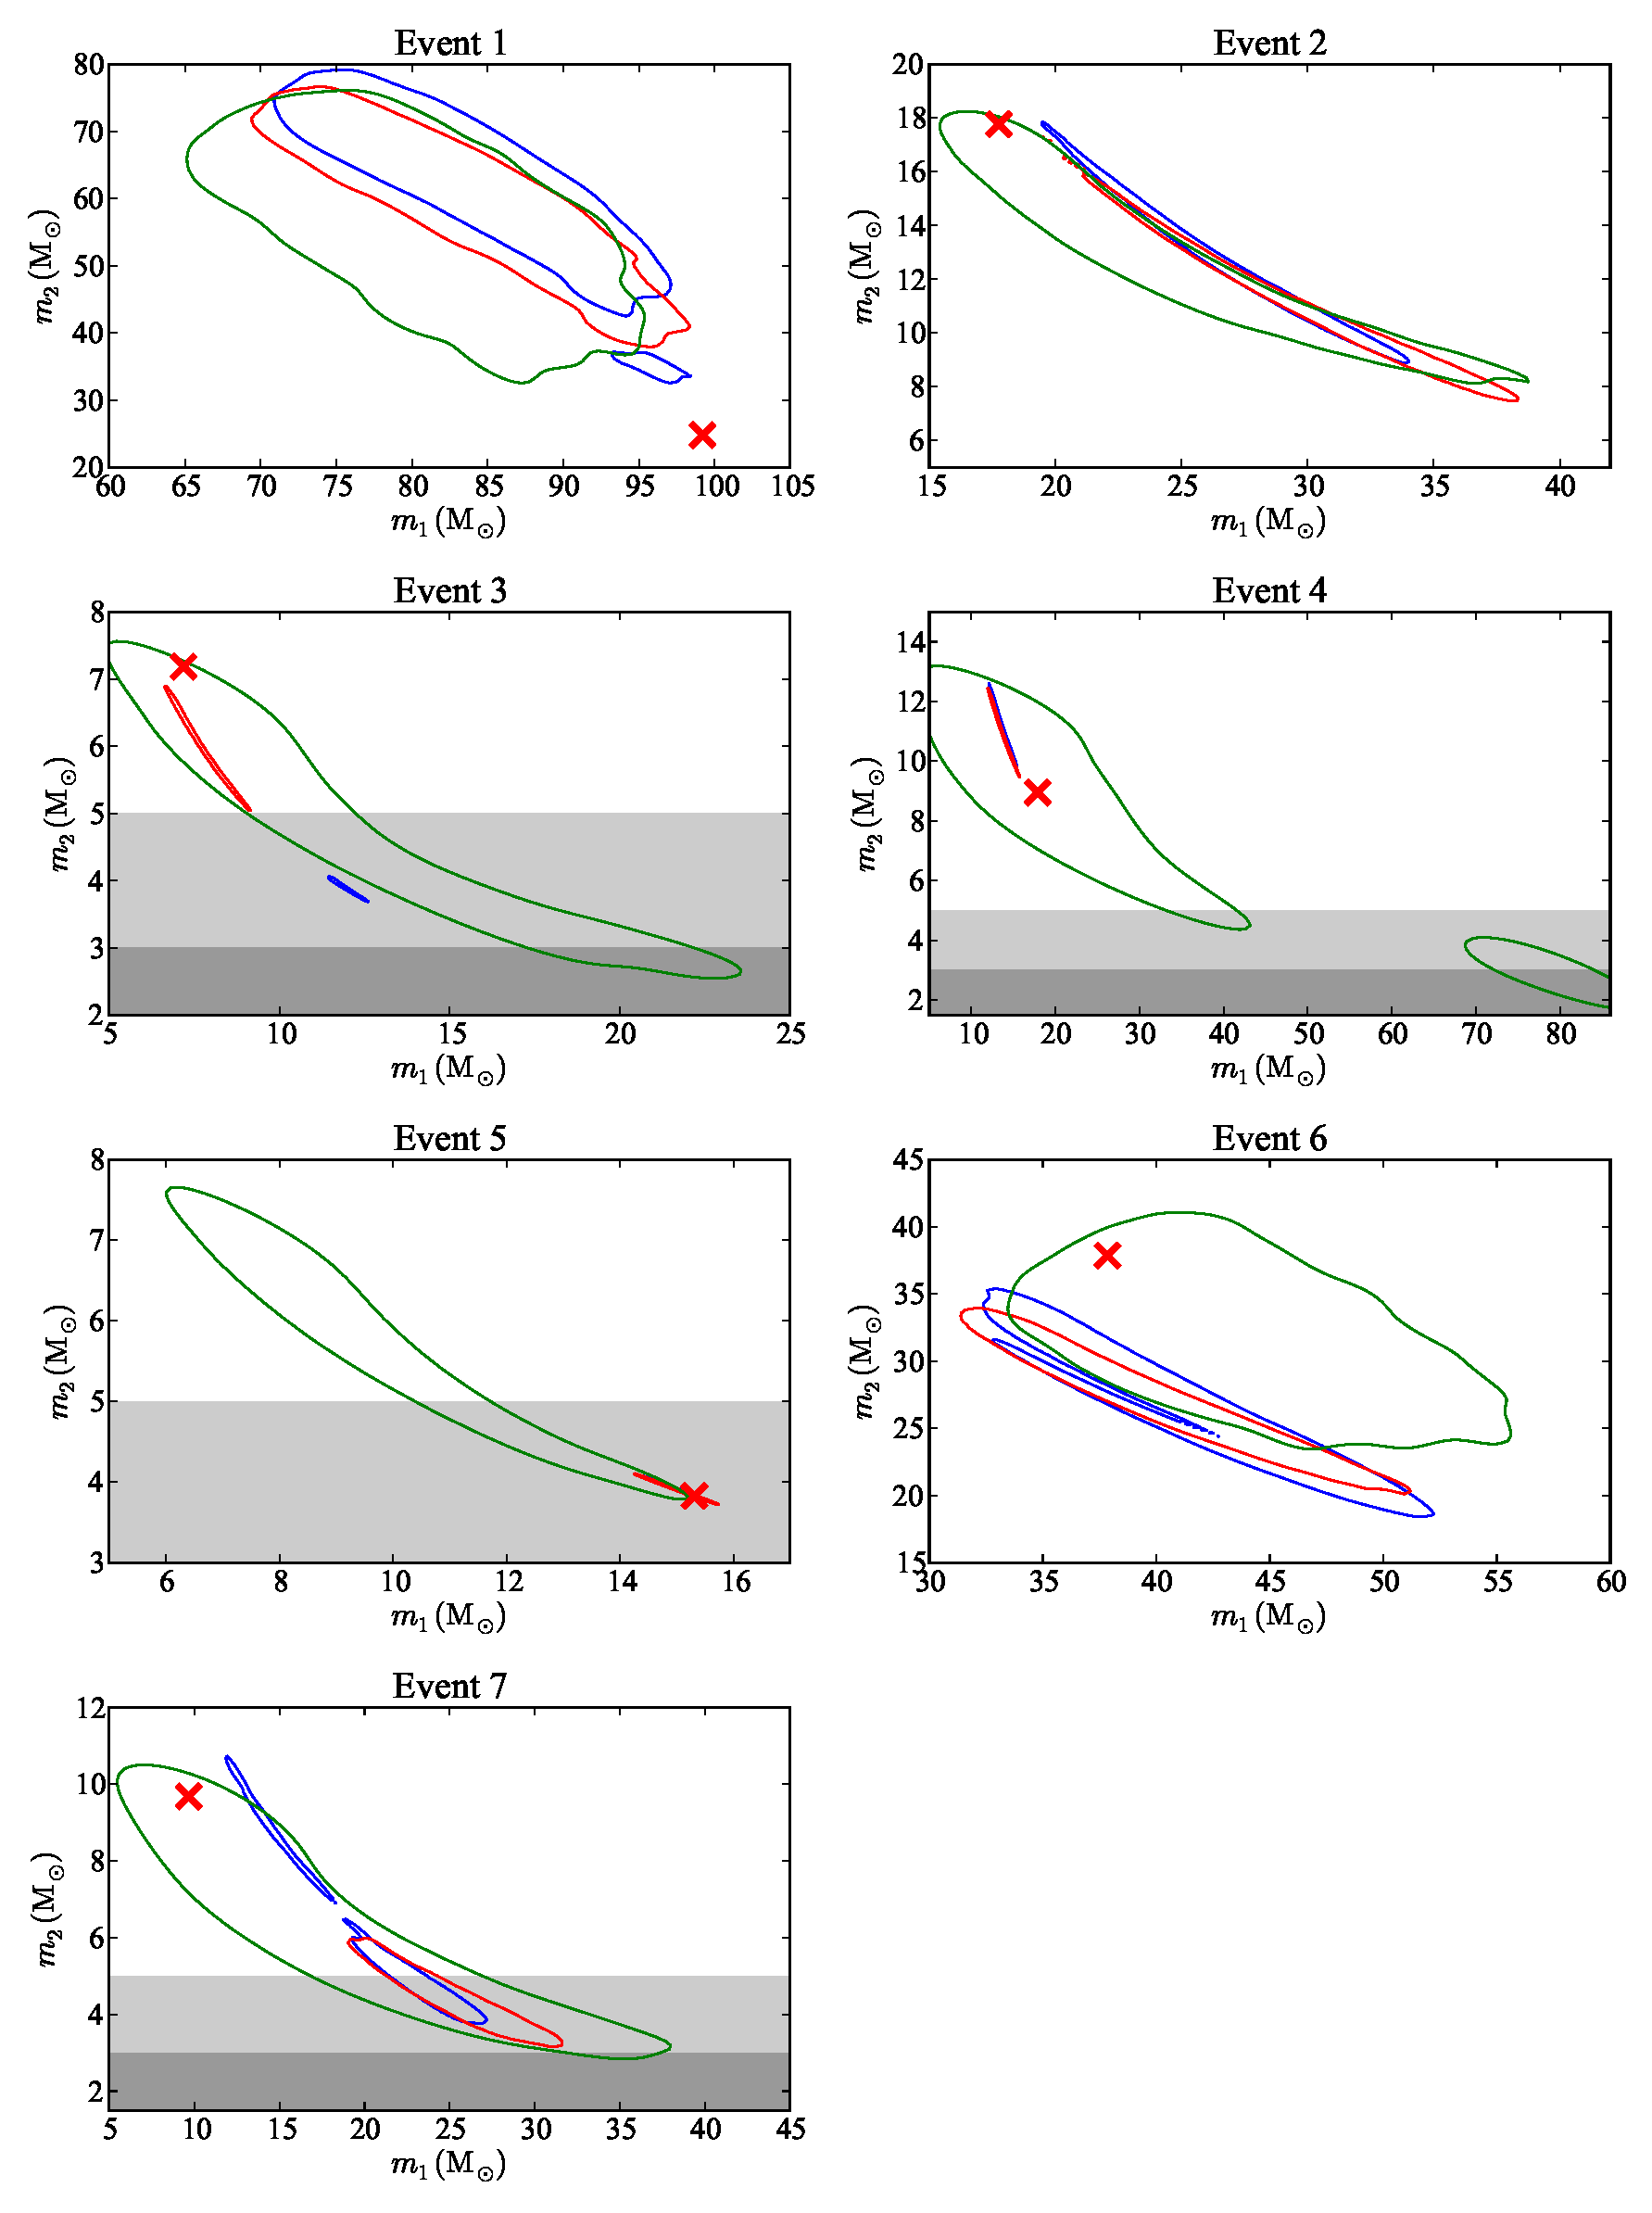
\includegraphics[width=\textwidth]{figs/chapter3/figure6}
\caption{\label{fig:ratecomparebns} A comparison of the \ac{O1} 90\% upper limit on the
\ac{BNS} merger rate to other rates discussed in the text \protect\citep{
Abadie:2010cf, Kim:2013tca, Fong:2015oha, Siellez:2013hia, Coward:2012gn,
Petrillo:2012ij, Jin:2015txa, Vangioni:2015ofa, deMink:2015yea, Dominik:2014yma}.  The region excluded by the low-spin \ac{BNS} rate limit is
shaded in blue.  Continued non-detection in O2 (slash) and O3 (dot) with higher
sensitivities and longer operation time would imply stronger upper limits.  The
O2 and O3 \ac{BNS} ranges are assumed to be 1-1.9 and 1.9-2.7 times larger than
\ac{O1}.  The operation times are assumed to be 6 and 9
months~\citep{Aasi:2013wya} with a duty cycle equal to that of \ac{O1} ($\sim$ 40\%).}
\end{figure}

\begin{figure}[t]
\centering
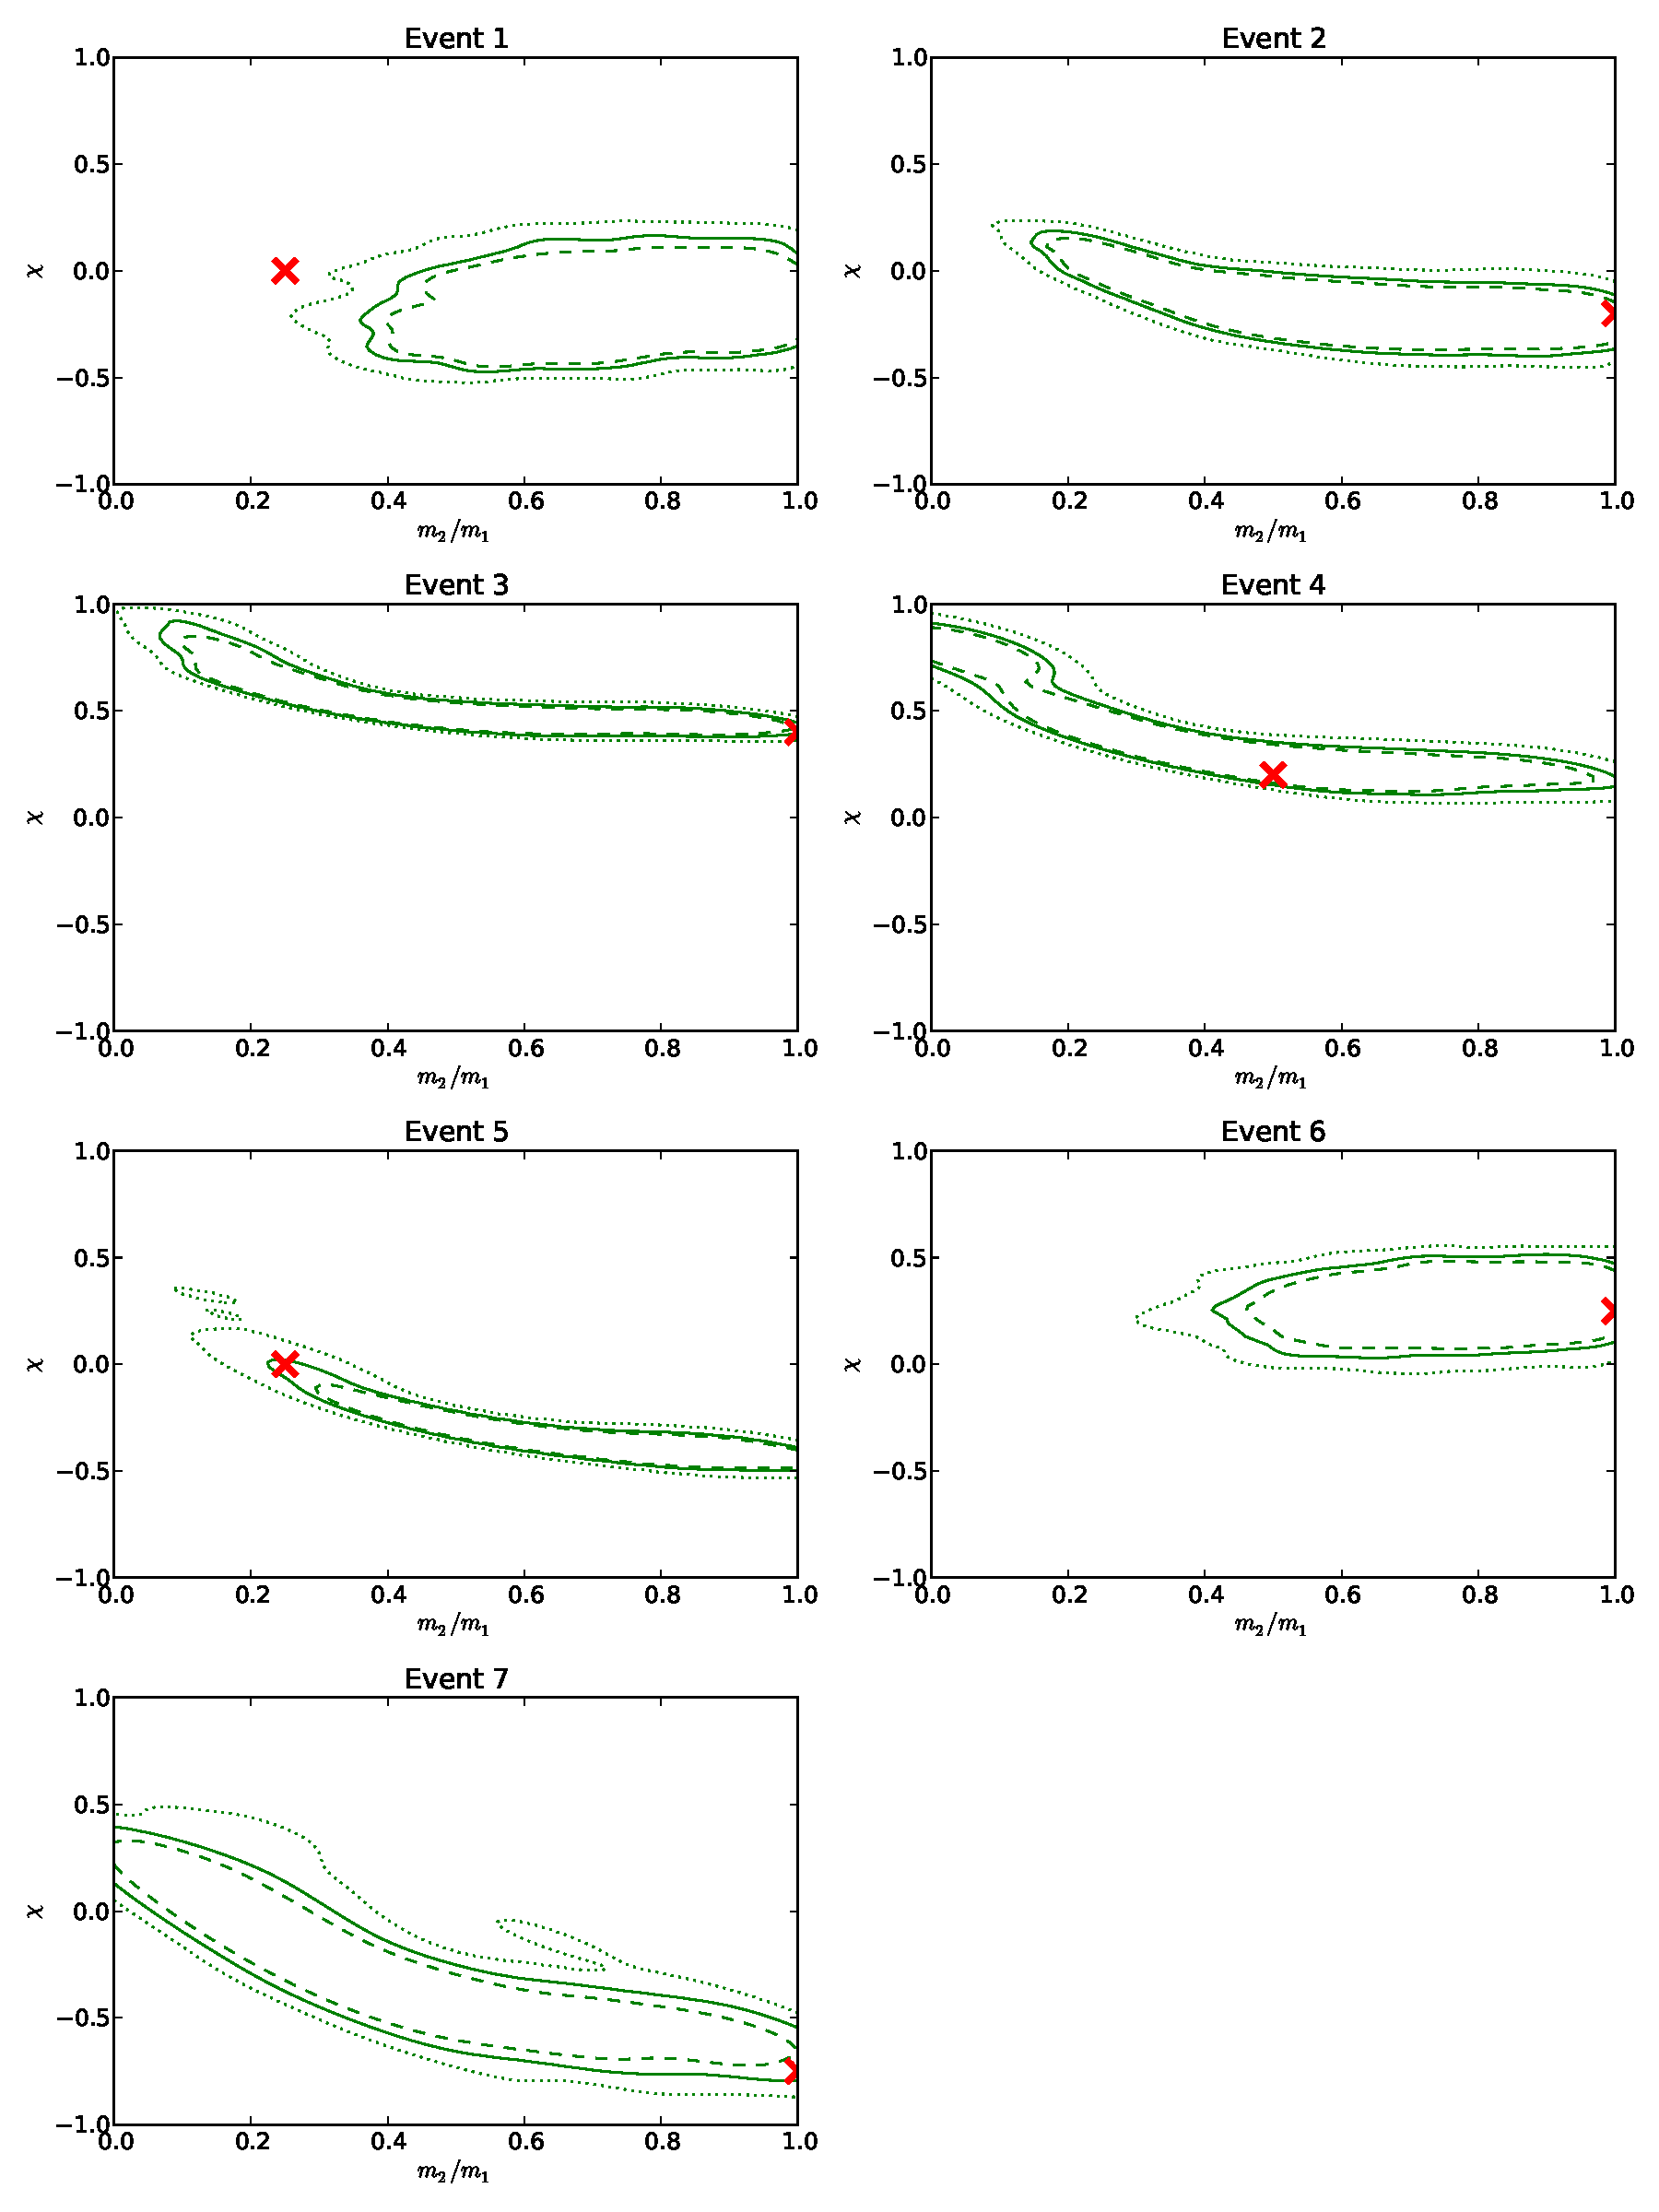
\includegraphics[width=\textwidth]{figs/chapter3/figure7}
\caption{\label{fig:ratecomparensbh} A comparison of the \ac{O1} 90\% upper limit on
the \ac{NSBH} merger rate to other rates discussed in
the text \protect\citep{Abadie:2010cf, Fong:2015oha, Coward:2012gn,
Petrillo:2012ij, Jin:2015txa, Vangioni:2015ofa, deMink:2015yea, Dominik:2014yma}.
The dark blue region assumes a \ac{NSBH} population with masses 5--1.4 $M_{\odot}$ and the
light blue region assumes a \ac{NSBH} population with masses 10--1.4 $M_{\odot}$.
Both assume an isotropic spin distribution.
Continued non-detection in O2 (slash) and O3 (dot) with higher sensitivities and longer
operation time would imply stronger upper limits (shown for 10--1.4 $M_{\odot}$ \ac{NSBH}
systems).
The O2 and O3 ranges are assumed to be 1-1.9 and 1.9-2.7 times larger than
\ac{O1}.
The operation times are assumed to be 6 and 9 months~\citep{Aasi:2013wya}
with a duty cycle equal to that of \ac{O1} ($\sim$ 40\%).}
\end{figure}

\begin{figure}[t]
\centering
\includegraphics[width=\textwidth]{figs/chapter3/figure8.pdf}
\caption{\label{fig:beaming} Lower limit on the beaming angle of short
\acp{GRB}, as a function of the mass of the primary BH or
NS, $m_1$. We take the appropriate  90\% rate upper limit from this paper,
assume all short \acp{GRB} are produced by each case in turn, and assume all
have the same beaming angle $\theta_j$. The limit is calculated using an
observed short \ac{GRB} rate of
$10^{+20}_{-7}$Gpc$^{-3}$ yr$^{-1}$
and the ranges shown on the plot reflect the uncertainty in this observed rate.
For \ac{BNS}, $m_2$ comes from a Gaussian distribution centered on $1.35M_\odot$, and
for \ac{NSBH} it is fixed to $1.4M_\odot$.}
\end{figure}

We can compare our upper limits with rate predictions for compact object mergers
involving \acp{NS}, shown for \ac{BNS} in Figure~\ref{fig:ratecomparebns} and for \ac{NSBH} in
Figure~\ref{fig:ratecomparensbh}. A wide range of predictions derived from population
synthesis and from binary pulsar observations were reviewed in 2010 to produce rate estimates
for canonical
$1.4\,{{M_{\odot}}}$ \acp{NS} and $10\,{{M_{\odot}}}$ \acp{BH}~\citep{Abadie:2010cf}. We
additionally include some more recent estimates from population synthesis for
both \ac{NSBH} and \ac{BNS} \citep{Dominik:2014yma,Belczynski:2015tba,deMink:2015yea} and
binary pulsar observations for \ac{BNS} \citep{Kim:2013tca}.

We also compare our upper limits for \ac{NSBH} and \ac{BNS} systems to beaming-corrected
estimates of short \ac{GRB} rates in the local universe. Short \acp{GRB} are
considered likely to be produced by the merger of compact
binaries that include \acp{NS}, i.e. \ac{BNS} or \ac{NSBH}
systems~\citep{Berger:2013jza}. The rate of short \acp{GRB} can
predict the rate of progenitor mergers %\ac{BNS} and/or \ac{NSBH} systems
\citep{Coward:2012gn,Petrillo:2012ij,Siellez:2013hia,Fong:2015oha}.
For \ac{NSBH}, systems with small \ac{BH} masses are considered more likely to be able to
produce short \acp{GRB} (e.g.~ \citep{Duez:2009yz,Giacomazzo:2012zt,Pannarale:2015jia}), so we compare to our
$5 M_{\odot}$--$1.4 M_{\odot}$
\ac{NSBH} rate constraint. The observation of a kilonova is also considered to be an
indicator of a binary merger~\citep{Metzger:2011bv}, and an estimated kilonova rate
gives an additional lower bound on compact binary mergers~\citep{Jin:2015txa}.

Finally, some recent work has used the idea that mergers involving \acp{NS}
are the primary astrophysical source of r-process
elements \citep{1974ApJ...192L.145L,Qian:2007vq} to constrain the rate of such
mergers from nucleosynthesis \citep{Bauswein:2014vfa,Vangioni:2015ofa}, and we
include rates from \citep{Vangioni:2015ofa} for comparison.

While limits from \ac{O1} are not yet in tension with astrophysical models, scaling
our results to current expectations for advanced \ac{LIGO}'s next two observing runs,
O2 and O3 \citep{Aasi:2013wya}, suggests that significant constraints or
observations of \ac{BNS} or \ac{NSBH} mergers are possible in the next two years.

Assuming that short \acp{GRB} are produced by \ac{BNS} or \ac{NSBH}, but
without using beaming angle estimates, we can constrain the beaming angle of the jet
of gamma rays emitted from these \acp{GRB} by comparing the rates of
\ac{BNS}/\ac{NSBH} mergers and the rates of
short \acp{GRB}~\citep{Chen:2012qh}.
For simplicity, we assume here that all short \acp{GRB} are associated with \ac{BNS}
or \ac{NSBH} mergers; the true fraction will
depend on the emission mechanism.  The short \ac{GRB} rate $R_{GRB}$, the merger rate
$R_{merger}$, and the beaming angle $\theta_j$ are then related by
%
\begin{linenomath*}
\begin{equation}\label{eq:beaming}
\cos \theta_j = 1 - \frac{R_{\mathrm{GRB}}}{R_{\mathrm{merger}}}
\end{equation}
\end{linenomath*}

%
We take $R_{GRB}=10^{+20}_{-7}$Gpc$^{-3}$
yr$^{-1}$~\citep{Coward:2012gn,Nakar:2005bs}.
Figure~\ref{fig:beaming} shows the resulting \ac{GRB} beaming lower limits for the
90\% \ac{BNS} and \ac{NSBH} rate upper limits.
With our assumption that all short \ac{GRB}s are produced by a single progenitor
class, the constraint is tighter for \ac{NSBH} with larger
\ac{BH} mass.
Observed \ac{GRB} beaming angles are in the range of
$3-25^{\circ}$~\citep{Fox:2005kv,Fong:2015oha,Grupe:2006uc,Soderberg:2006bn,2013ApJ...766...41S,2012ApJ...756...63M,2011A&A...531L...6N}.
Compared to the lower limit derived from our non-detection, these \ac{GRB}
beaming observations start to confine the fraction of \ac{GRB}s that can be
produced by higher-mass NSBH as progenitor systems.
Future constraints could also come from \ac{GRB} and \ac{BNS} or \ac{NSBH} joint
detections~\citep{Dietz:2010eh,Regimbau:2014nxa, Clark:2014jpa}.

\newpage

\begin{sidewaystable}
  \centering
  \begin{tabular}{c|c|c|c|c}
   \hline\hline
   Injection & Range of spin  & $\langle VT \rangle$ (Gpc$^3$~yr) & Range (Mpc) & $R_{90\%}$ (Gpc$^{-3}$~yr$^{-1}$) \\
   \hline \hline
   Isotropic low spin & [0, 0.05] & \MainBNSVTPyCBCLowSpin & \MainBNSRangePyCBCLowSpin &  \MainBNSULPyCBCLowSpin \\
   Isotropic high spin & [0, 0.4] & \MainBNSVTPyCBCHighSpin & \MainBNSRangePyCBCHighSpin & \MainBNSULPyCBCHighSpin \\
   \hline\hline
  \end{tabular}
  \caption{\label{tab:bns_ul_table} Sensitive space-time volume $\langle VT \rangle$ and 90\% confidence upper
  limit $R_{90\%}$ for \ac{BNS} systems. Component
  masses are sampled from a normal distribution $\mathcal{N}(1.35M_\odot, (0.13M_\odot)^2$) with samples outside the
  range $[1, 3]M_{\odot}$ removed. Values are shown for the \texttt{pycbc}
  pipeline. $\langle VT \rangle$ is calculated using a FAR threshold of 0.01~yr$^{-1}$. The
  rate upper limit is calculated using a uniform prior on $\Lambda = R \langle
VT \rangle$ and an 18\% uncertainty in $\langle VT \rangle$ from calibration errors.}
\end{sidewaystable}

\newpage

\begin{sidewaystable}
  \centering
  \begin{tabular}{c|c|c|c|c|c}
   \hline\hline
   NS mass & BH mass & Spin & $\langle VT \rangle$ (Gpc$^3$~yr) & Range (Mpc) & $R_{90\%}$ (Gpc$^{-3}$~yr$^{-1}$) \\
   ($M_\odot$) & ($M_\odot$) & distribution &  & &  \\
   \hline \hline
   1.4 & 5 & Isotropic & \MainNSBHVTPyCBCFiveIso & \MainNSBHRangePyCBCFiveIso & \MainNSBHULPyCBCFiveIso \\
   1.4 & 5 & Aligned & \MainNSBHVTPyCBCFiveAligned & \MainNSBHRangePyCBCFiveAligned & \MainNSBHULPyCBCFiveAligned \\
   1.4 & 10 & Isotropic & \MainNSBHVTPyCBCTenIso & \MainNSBHRangePyCBCTenIso & \MainNSBHULPyCBCTenIso \\
   1.4 & 10 & Aligned & \MainNSBHVTPyCBCTenAligned & \MainNSBHRangePyCBCTenAligned & \MainNSBHULPyCBCTenAligned  \\
   1.4 & 30 & Isotropic & \MainNSBHVTPyCBCThirtyIso & \MainNSBHRangePyCBCThirtyIso & \MainNSBHULPyCBCThirtyIso \\
   1.4 & 30 & Aligned & \MainNSBHVTPyCBCThirtyAligned & \MainNSBHRangePyCBCThirtyAligned & \MainNSBHULPyCBCThirtyAligned \\
   \hline\hline
  \end{tabular}
  \caption{\label{tab:nsbh_ul_table} Sensitive space-time volume $\langle VT \rangle$ and 90\% confidence upper
  limit $R_{90\%}$ for \ac{NSBH} systems with isotropic and aligned spin distributions. The NS spin magnitudes
  are in the range $[0, 0.04]$ and the BH spin magnitudes are in the range $[0, 1]$. Values are shown for the \texttt{pycbc}
  pipeline. $\langle VT \rangle$ is calculated using a FAR threshold of 0.01~yr$^{-1}$. The
  rate upper limit is calculated using a uniform prior on $\Lambda = R \langle
VT \rangle$ and an 18\% uncertainty
  in $\langle VT \rangle$ from calibration errors.}
\end{sidewaystable}


\Chapter{First Open Gravitational wave Catalog : 1-OGC}
\label{ch:1_OGC}
\newcommand{\note}[1]{{\color{red} [#1]}}
\def\cn{\note{cite}}

\newcommand{\chieff}{\ensuremath{\chi_{\mathrm{eff}}}}
\newcommand{\rankingstat}{\ensuremath{\tilde{\rho}_c}}
\newcommand{\tdr}{\ensuremath{\mathrm{TDR}}}
\newcommand{\far}{\ensuremath{\mathcal{F}}}
\newcommand{\tar}{\ensuremath{\mathcal{T}}}
\newcommand{\msun}{\ensuremath{\mathrm{M}_{\odot}}}
\newcommand{\pastro}{\ensuremath{P_{\mathrm{astro}}}}
\newcommand{\release}{\texttt{\url{www.github.com/gwastro/1-ogc}}}

\section{Introduction}
\label{sec:intro}
The following chapter is taken from work presented in \cite{nitz20191}.

The Advanced LIGO gravitational wave observatories~\citep{Martynov:2016fzi} performed their first observing run (O1) from September 12, 2015 to January 19, 2016. This provided a total of 51.5 days of coincident observations from the two detectors located in Hanford, WA and Livingston, LA. The binary black hole mergers observed in this observing run have been  reported by the LIGO and Virgo Collaborations (LVC) in \cite{Abbott:2016blz,Abbott:2016nmj,TheLIGOScientific:2016pea}.  These binary black hole detections have been independently studied by \cite{Green:2017voq,Roulet:2018jbe,Antelis:2018smo}.

Since the publication of the results by \cite{TheLIGOScientific:2016pea,Abbott:2016ymx}, improvements to the data-analysis methods used~\citep{TheLIGOScientific:2016qqj} have been implemented \citep{Nitz:2017svb,Nitz:2017lco,DalCanton:2017ala}.  Using these improvements, we re-analyze the O1 data and provide---for the first time---a full catalog of candidate events from a matched filter search for compact binary coalescences using the O1 data, which we call 1-OGC. This catalog provides estimates of the significance of previously known events and a ranked list of sub-threshold candidates. Although not significant by themselves, these sub-threshold candidates can be correlated with archival data or transient events found by other astronomical observatories to provide constraints on the population of compact-object mergers \citep{Ashton:2017ykh, Burns:2018pcl}.

Our catalog is based entirely on public, open data and software. We use the LIGO data available from the Gravitational Wave Open Science Center~\citep{Vallisneri:2014vxa}, and analyze the data using the open source PyCBC toolkit~\citep{Usman:2015kfa,Canton:2014ena,pycbc-github}.This toolkit was also used by one of the two analyses described in~\cite{TheLIGOScientific:2016qqj}. The lowest mass sources targeted in our search are neutron star binaries with total mass $m_1 + m_2 = 2\, M_\odot$. The search space extends to binary black hole systems that produce gravitational waveforms longer than $0.15$~s from $20$~Hz. This corresponds to a total mass up to $500 M_{\odot}$ for sources with high mass ratios and spins where the component aligned with the orbital angular momentum is positive and large. For binaries with negligible spin, this corresponds to total mass $\lesssim 200 M_{\odot}$. The search space also includes neutron star--black hole binaries. After applying cuts for data quality~\citep{TheLIGOScientific:2016zmo,TheLIGOScientific:2017lwt}, a total of 48.1~days of coincident data are searched for signals.

The three most significant signals in the catalog correspond to GW150914~\citep{Abbott:2016blz}, LVT151012~\citep{Abbott:2016blz,TheLIGOScientific:2016pea}, and GW151226~\citep{Abbott:2016nmj}, respectively. No other astrophysically significant signals are observed. In the analysis of \cite{TheLIGOScientific:2016pea}, LVT151012 was the third-most significant event, but it was not sufficiently significant to be labeled as an unambiguous detection. With the improved methods employed here, the false alarm rate of this candidate improves by an order of magnitude and it should be considered a true astrophysical event. The analyses of \cite{TheLIGOScientific:2016pea,Abbott:2016ymx} restricted the astrophysical search space to binaries with a total mass less that $100\,M_\odot$. Our analysis extends this target space to higher mass signals. No additional signals are detected in this region of parameter space, consistent with the results of \cite{Abbott:2017iws}. 

A second observing run (O2) of the Advanced LIGO detectors took place from November 30, 2016 to August 25, 2017~\citep{Aasi:2013wya}.  The Virgo gravitational wave detector also collected data for part of this period, starting from August 1, 2017.  The detections reported in this second observing run thus far include nary black hole coalescence even three additional binary black hole coalescence events \citep{Abbott:2017vtc,Abbott:2017gyy,Abbott:2017oio}, and a binary neutron star merger \citep{TheLIGOScientific:2017qsa}. However, the full O2 data set has not yet been released. The catalog presented here is therefore restricted to the first observing run, O1.

Our paper is organized as follows: In Sec.~\ref{sec:search} and Sec.~\ref{sec:tdr}, we summarize our analysis methods, including the parameter space searched, the detection statistic used for ranking candidate events, and our method for calculating the statistical significance of events. The search results are summarized in Sec.~\ref{sec:results}.  Our full catalog and released data are
described in Sec.~\ref{sec:datarelease} and are available online as supplementary materials (\release). In this paper, we focus on the detection of compact objects. Since no new astrophysical events have been observed, we do not consider measurement of the signals' parameters and refer to \cite{TheLIGOScientific:2016pea,Biwer:2018osg} for discussion of the detected events' source-frame properties. Consequently, we quote binary mass parameters in the detector frame in this work.

\section{Search Methodology}
\label{sec:search}

To search for gravitational waves from compact-object mergers, we use matched filtering~\citep{Allen:2005fk} implemented in the open-source PyCBC library~\citep{Usman:2015kfa,Canton:2014ena,pycbc-github}. Our methods improve on the analyses of \cite{TheLIGOScientific:2016pea,Abbott:2016ymx,TheLIGOScientific:2016qqj} by imposing a phase, amplitude and time delay consistency on candidate signals, an improved background model, and a larger search parameter space~\citep{Nitz:2017svb, Nitz:2017lco, DalCanton:2017ala}.

\begin{figure}[h]
  \centering
    \includegraphics[width=\columnwidth]{figs/chapter5/bank.pdf}
\caption{The component masses and spins of the templates used to search for compact binary mergers. Due to the exclusion of short duration templates, there is a dependency on the total mass searched and its effective spin. For binary black holes with negligible spin, this implies that this study only probes sources with total mass less than ~$200\,\msun$. Visible artifacts due to the procedure for constructing the template bank do not impact performance. Templates which we conservatively consider to produce binary black hole (BBH) candidates consistent with known observations are shown in red as discussed in Sec.~\ref{sec:tdr}. The upper mass boundary of the analysis performed by the LVC in~\cite{TheLIGOScientific:2016pea} is shown
as a black dotted line.}
\label{fig:bank}
\end{figure}

\subsection{Target Search Space}

A discrete bank of gravitational-wave template waveforms~\citep{Owen:1995tm,Owen:1998dk,Brown:2012qf} is used to target binary neutron star,
neutron star--black hole, and binary black hole mergers with total mass from $2-500 M_{\odot}$~\citep{DalCanton:2017ala}. The templates are
parameterized by their component masses $m_{1,2}$ and their dimensionless spins  $\vec{\chi}_{1,2} = c \vec{S}_{1,2}/G m_{1,2}^2$, where
$\vec{S}_{1,2}$ are the spin vectors of each compact object.  For compact objects with component
masses greater than $2 M_{\odot}$, the template bank covers a wide range of spins, with $\chi_{(1,2)z} \in [\pm 0.998]$, where $\chi_{(1,2)z}$ are the components aligned with the orbital angular momentum. For compact objects
with masses less than  $2 M_{\odot}$, the spin is restricted to $\chi_{(1,2)z} \in [\pm 0.05]$~\citep{Brown:2012qf}. Templates that correspond
to sources with a signal duration less than 0.15 seconds (starting from $20\,$Hz) are excluded due to the difficulty in separating candidates arising from
these templates from populations of instrumental glitches~\citep{DalCanton:2017ala}. Consequently, the total mass boundary of the search
depends strongly on the ``effective spin" \citep{Racine:2008qv, Ajith:2009bn},
%
\begin{equation}
\chieff = \frac{\chi_{1z} m_1 + \chi_{2z} m_2}{m_1+m_2}.
\end{equation}
%
This dependence is visible in the distribution of the approximately $400,000$ templates required to cover the space shown in Fig.~\ref{fig:bank}. A dotted line in Fig.~\ref{fig:bank} denotes the upper boundary of the O1 analysis performed in~\cite{TheLIGOScientific:2016pea}. For binaries with total mass greater than $4\,M_\odot$, we use the spinning effective-one-body model (SEOBNRv4)~\citep{Taracchini:2013,Bohe:2016gbl} as template gravitational waveforms. For sources with total masses less than $4M_{\odot}$ we use TaylorF2 post-Newtonian waveforms with phasing accurate to 3.5 post-Newtonian order and the dominant amplitude evolution~\citep{Sathyaprakash:1991mt,Droz:1999qx,Blanchet:2002av,Faye:2012we}. Our choice of template bank discretization causes less than a $10\%$ loss in detection rate for any source within the boundaries of the template bank. Our search assumes that the source can be adequately described by only the dominant gravitational-wave mode, two component masses, non-precessing spins, and negligible eccentricity.

\subsection{Creation and Ranking of Candidate Events}

For each template and each detector, we calculate the matched filter signal-to-noise ratio (SNR) as a function of time $\rho(t)$~\citep{Allen:2005fk}. The template bank is divided into 15 equal sized sub-banks based on the chirp mass $\mathcal{M} = (m_1m_2)^{3/5} / (m_1+m_2)^{1/5}$ of each template. A single-detector ``trigger" is a peak in the SNR time series that is greater than 4 and larger than any other peaks within 1s. For each sub-bank, the loudest 100 triggers (by $\rho$) are recorded in $\sim1$s fixed time windows. This method has been shown to improve search sensitivity, while making the rate of single-detector triggers manageable~\citep{Nitz:2018rgo}. We have found this choice of sub-banks to be an effective method to ensure the analysis can concurrently record triggers from separate regions of parameter space that respond differently to instrumental noise. Other choices are possible.

 We use the data-quality segments provided by the Gravitational-Wave Open Science Center to exclude triggers that occur in times when there are problems with the detectors' data quality~\citep{TheLIGOScientific:2016zmo,TheLIGOScientific:2017lwt}.
 In addition, very loud transient glitches, corresponding to $>100\sigma$ deviations from Gaussian noise, are excised from the strain data according to the procedure of~\cite{Usman:2015kfa} before calculation of the SNR time series. However, there remain many types of transient non-Gaussian noise in the LIGO data which produce triggers with large values of SNR~\citep{Nuttall:2015dqa,TheLIGOScientific:2016zmo,TheLIGOScientific:2017lwt}. 

 For every trigger with $\rho > 5.5$ we calculate the signal consistency test, $\chi^2_r$, introduced in~\cite{Allen:2004gu}. The statistic $\chi^2_r$ divides the matched filter into frequency bands and checks that the contribution from each band is consistent with the expected signal. The statistic takes values close to unity when the data contains either Gaussian noise or the expected signal and larger values for many types of transient glitches. We impose the SNR limit as the $\chi^2_r$ test is generally non-informative when $\rho < 5.5$. The $\chi^2_r$ value is used to re-weight the SNR $\rho$ as~\citep{Babak:2012zx}
%
\begin{equation}
 \tilde{\rho} = \begin{cases} 
        \rho & \mathrm{for}\ \chi^2_r \leq 1 \\
        \rho\left[ \frac{1}{2} \left(1 + \left(\chi^2_r\right)^3\right)\right]^{-1/6}, & 
        \mathrm{for}\ \chi^2_r > 1.
    \end{cases}
\end{equation}
%

For single-detector triggers from templates with total mass greater than 40$M_{\odot}$ we apply an additional test, $\chi^2_{r,sg}$, that determines if the detector output contains power at higher frequencies than the maximum expected frequency content of the gravitational-wave signal~\citep{Nitz:2017lco}. This test is only applied for higher mass systems, since these templates are shorter in duration and more difficult to separate from instrumental noise. For other systems, we set $\chi^2_{r,sg} = 1$. Using this statistic, we apply a further re-weighting as
%
\begin{equation}
\label{eq:sg}
 \hat{\rho} = \begin{cases} 
        \tilde{\rho} & \mathrm{for}\ \chi^2_{r,sg} \leq 4 \\
        \tilde{\rho} (\chi^2_{r,sg} / 4)^{-1/2}, & 
        \mathrm{for}\ \chi^2_{r,sg} > 4.
    \end{cases}
\end{equation}

Candidate events are generated when single-detector triggers occur in both the LIGO Hanford and Livingston data within $12$~ms (the light-travel time between the observatories extended by $2$~ms for signal time-measurement error) and if the triggers are recorded in the same template in each detector~\citep{Usman:2015kfa}.  Following the procedure of~\cite{Nitz:2017svb}, we model the distribution of single detector triggers from each template as an exponentially decaying function, $\lambda(\hat{\rho}, \vec{\theta}^N)$, where $\vec{\theta}^N$ allows the parameters of the exponential to vary as a function of total mass, symmetric mass ratio $\eta=m_1m_2/M^2$, and $\chieff$. This fitted model allows us to rescale $\hat{\rho}$ to better equalize the rate of triggers from each template.

We improve upon the ranking of candidates in~\cite{Abbott:2016ymx,TheLIGOScientific:2016pea} by also taking into account $p^S(\vec{\theta}^S)$, which is the expected distribution of SNR $\rho_H$ and $\rho_L$, phase difference $\phi_{c, H} - \phi_{c, L}$, and arrival time delay $t_{c,H} - t_{c,L}$ between the two LIGO instruments for an astrophysical population~\citep{Nitz:2017svb}. No assumption is made about the distribution of intrinsic source parameters in this term. The primary benefit arises from assuming the population of sources is isotropically distributed in orientation and sky location. The final ranking statistic \rankingstat{} is then calculated as
\begin{equation}\label{eq:genstat}
  \rankingstat \propto \left[ \log p^S(\vec{\theta}^S) - \log \left(\lambda_H(\hat{\rho}_{H},\vec{\theta}^N) \lambda_L(\hat{\rho}_{L}, \vec{\theta}^N)\right) 
  \right] + \mathrm{const.}
\end{equation}
This expression is normalized so that \rankingstat{} approximates the standard network SNR $\rho_c = (\rho_L^2 + \rho_H^2)^{1/2}$ for candidates from regions of parameter space that are not affected by elevated rates of instrumental noise. Candidates from regions affected by elevated rates of noise triggers are down-weighted and assigned a smaller statistic value by this method. As multiple candidates, which arise from different template waveforms, may occur in response to the same signal, we select only the highest ranked candidate within ten seconds. A simpler version of this statistic where the single-detector exponential noise model is only a function of the template duration has also been employed in the analysis of data from LIGO's second observing run~\citep{GW170104, GW170814, Abbott:2017gyy}.

\subsection{Statistical Significance}

The statistical significance of candidate events is estimated by measuring empirically the rate of false alarms (FAR). To measure the noise background rate, we generate additional analyses by time shifting the data from one instrument with respect to the other by multiples of 100 ms. Since this time shift is greater than the maximum astrophysical time of flight between observatories, any candidates produced in these analyses are false alarms. This time shift is much greater than the auto-correlation length of our template waveforms of $\mathcal{O}$(1ms). The time-slid analyses are produced following the same procedure as the search; This is a key requirement for our analysis to produce valid statistical results~\citep{TheLIGOScientific:2016qqj}. The equivalent of more than 50,000 years of observing time can be generated from 5 days of data.

To provide an unbiased measure of the rate of false alarms at least as significant as a potential candidate, the single-detector triggers that compose the candidate event should be included in the background estimation~\citep{2017PhRvD..96h2002C}. However, when a real signal with a large \rankingstat{} is present in the data, the rate of false alarms for candidate events with smaller \rankingstat{} tends to be overestimated. This is due to the fact that the loud single-detector triggers from the real event in one detector form coincidences with noise fluctuations in the other detector, producing loud coincident background events. As in \cite{TheLIGOScientific:2016pea}, an unbiased rate of false alarms can be achieved by a hierarchical procedure whereby a candidate with large \rankingstat{} is removed from the estimation of background for candidates with smaller \rankingstat{}; we use this procedure here.

NEED TO EXPAND THIS PART

\section{Evaluating Candidates based on the Astrophysical Population}
\label{sec:tdr} 

We find two candidate events with
FAR $< 1$ per $50\,000$ years, corresponding to GW150914 and GW151226.
Although FAR does not give the probability that an event is an astrophysical signal,
we can be confident that these events were not caused by chance
coincidence between the detectors. It is possible that these
events were caused by a correlated source between the detectors. However, detailed followup
studies of GW150914 and GW151226 found no correlated noise sources between the detectors
that could be mistaken for a gravitational wave \citep{TheLIGOScientific:2016zmo, Abbott:2016nmj}.

We conclude that GW150914 and GW151226 are astrophysical in origin and use them to constrain the rate of real signals. A ``true discovery rate"
(\tdr{}) can be constructed for less significant events. The \tdr{} is defined as:
%
\begin{equation}
\tdr(\rankingstat) = \frac{\tar(\rankingstat)}{\tar(\rankingstat) + \far(\rankingstat)},
\end{equation}
%
where $\tar(\rankingstat)$ is the rate that signals of astrophysical origin are observed with
a ranking statistic $\geq \rankingstat$ (the ``true alarm rate") and
$\far(\rankingstat)$ is the false alarm rate.

The true discovery rate is the complement of the false discovery rate~\citep{Benjamini:1995ram},
and can be used to estimate the fraction of real signals in a population.
For example, if $\tdr(\rankingstat) = 0.9$, it means that
$90\%$ of events with a ranking statistic $\geq \rankingstat$ are expected to be real signals.  The
\tdr{} is also independent of the observation time.

Note that \tdr{} is not the probability that a particular event is a signal of astrophysical origin \pastro{}. For that, one needs to model the distribution of signals and noise at a given \rankingstat{}. In this work, we use a simple model of these distributions as functions of the ranking statistic \rankingstat{}. Models incorporating additional parameters are also possible, but we do not consider them here. As a function of \rankingstat, \pastro{} can be computed as
%
\begin{equation}
\pastro(\rankingstat) = \frac{\Lambda_S P_S(\rankingstat)}{\Lambda_S P_S(\rankingstat) + \Lambda_N P_N(\rankingstat)},
\end{equation} 
%
where $P_S(\rankingstat)$ and $P_N(\rankingstat)$ are the probabilities of an event having ranking statistic \rankingstat{} 
given the signal and noise hypotheses respectively~\citep{2009MNRAS.396..165G,Farr:2015,Abbott:2016nhf}. $\Lambda_S$ and $\Lambda_N$ are the rates of signal and noise events.

Since no binary neutron star or neutron star--black hole candidates are obtained from a search of the O1 data, here we restrict the calculation of both the \tdr{} and \pastro{} to binary black hole (BBH) observations.
We include signals with total mass $M \geq 10\,\msun$, mass ratio $m_1/m_2 < 5$ (where $m_1 \geq m_2$),
and dimensionless spins $|\chi_{(1,2)z}| <
0.5$. These choices are based on a combination of what has been observed~\citep{TheLIGOScientific:2016pea,GW170104,GW170814,Abbott:2017gyy} and
what is expected from models of isolated binary-star evolution (``field"
binaries). The mass distribution of field binaries is dependent on a number of
unknown parameters, such as the metallicity of the environment~\citep{Belczynski:2014iua}. Generally, it is expected that most binaries are close to equal mass, as typically less than 1
in $\mathcal{O}(10^{3})$ simulated binaries have mass ratio $> 5$ in models of
field-binary evolution \citep{Dominik:2014yma}.  The majority of observations of
nearby X-ray binaries have yielded black holes with masses greater than
$5\,\msun$, which has led to speculation of a ``mass gap" between
3--5$\,\msun$ \citep{Ozel:2010su, Farr:2010tu, Kreidberg:2012ud}. The signals
detected so far by LIGO and Virgo are consistent with this: the smaller component mass
in the lowest-mass system known to date, GW170608, has an estimated mass of
$7^{+2}_{-2}\,\msun$ \citep{Abbott:2017gyy}.

The spin distribution of black holes is not well constrained~\citep{Reynolds:2013qqa}. The component spins
of the most significant binary black holes detected by LIGO and Virgo are
only weakly constrained \citep{TheLIGOScientific:2016pea}. The best measured
quantity related to spin is \chieff{}. All of the BBH gravitational-wave signals
detected so far have $|\chieff| \lesssim 0.2$. A binary with
low \chieff{} may still have component masses with large spin magnitudes,
if the spins are anti-parallel or are purely in the plane of the binary.
However, it seems unlikely that this would be the case for all of the
detections made so far. Hence we include signals that have
component spins with $|\chi_{(1,2)z}| < 0.5$. This is consistent with
recent population synthesis models, which indicate that black holes
must have low natal spin in order to obtain a distribution of \chieff{}
that satisfies gravitational-wave observations \citep{Belczynski:2017gds,Wysocki:2017isg}.

To estimate the rate and distribution of false alarms that arise only
from the region consistent with this selected population of
binary black hole mergers, we must determine which templates are sensitive to these sources.
It is necessary to analyze a simulated set of signals since
the template associated with a particular event is not guaranteed to share the 
true source parameters. We find that the region of the template bank defined by
$M > 8.5\,\msun$, $m_{1,2} > 2.7\,\msun$, and $\chieff < 0.9$ is effective at recovering
this population of sources. This region is shown in Fig.~\ref{fig:bank} in red. 

To estimate the true rate \tar{}, we use the two significant events observed
during O1, GW150914 and GW151226. We do not use any of the O2 events because the full data is
not yet available for analysis, making it difficult to obtain a consistent rate estimate. The total analysis time in O1 was $\sim48$ days, giving $\tar \approx 15 \mathrm{yr}^{-1}$. Given the uncertainty in
this estimate based on only two events, we take the rate of observations as a Poisson process, and choose the lower
95\% bound on \tar{}. This yields a $\tar \approx 2.7 \mathrm{yr}^{-1}$. For the calculation
of the \tdr{} we use this value for all events, independent of their ranking statistic. This means we likely underestimate the \tdr{} for events quieter than GW151226 and GW150914, but this is a conservative bias.

To estimate the probability that a given event is astrophysical in origin \pastro{}, we model
the distribution of signals and noise as a function of \rankingstat. It is reasonable to approximate the signal
probability distribution $P_S(\rankingstat)$ as $\propto \rankingstat^{-4}$~\citep{Schutz:2011tw,Chen:2014yla}.
We normalize the signal number density $\Lambda_S P_S(\rankingstat)$ so that the number of signals
with $\rankingstat$ greater than or equal to some threshold
$\rankingstat^{\dagger}$ is $\approx 2.7 \mathrm{yr}^{-1}$. We make the conservative choice to place
$\rankingstat^{\dagger}$ at the value of the next largest \rankingstat{} value after GW150914 and GW151226. 

To approximate the noise number density $\Lambda_N P_N(\rankingstat)$, we make a histogram of the \rankingstat{}
values of false alarms arising from our selected BBH region. We use only the false alarms which are uncorrelated
with possible candidate events to ensure an unbiased estimate of the mean false alarm rate~\citep{2017PhRvD..96h2002C}.
We fit an exponential decay to this histogram from $8<\rankingstat<9.2$. For \rankingstat{} much less than $8$,
$\Lambda_N P_N$ is not well modeled by an exponential due to the effects of applying a threshold to single-detector
triggers. We note, however, there is only a $ 50 \%$ chance that an event is astrophysical at
\rankingstat{} $\sim 8.6$, and this chance quickly becomes negligible with decreasing \rankingstat. The result of this
procedure is shown in Fig.~\ref{fig:pastro}. We caution that \pastro{} for candidates with
\rankingstat{} $>9.2$ will be sensitive to the form of the model chosen since it is not constrained by
empirically measured false alarms.

While we do not assess the astrophysical probabilities of sources outside our selected BBH region, we are not precluding that such sources exist.
Our \pastro{} is compatible with any model of the true BBH
source distribution that allows for a signal rate to be at least as high as our estimate within the chosen region. This holds irrespective of whatever other kinds of sources may also be permitted.

\begin{figure}[h]
  \centering
    \includegraphics[width=\columnwidth]{figs/chapter5/pastro.pdf}
\caption{The scaled probability distributions of assumed signals and noise as a function of the ranking statistic \rankingstat{} for the analysis containing LVT151012. Blue shows the normalized histogram of empirically measured false alarms that are within our selected BBH region of the template bank, $P_N$. Red is the exponential decay model that has been fitted to this set of false alarms, $P_S \Lambda_S / \Lambda_N$, normalized so that the counts can be directly compared to the noise distribution. Orange shows the signal model based on our conservative rate of detections. The value of \rankingstat{} for LVT151012 is shown as a dotted green vertical line. The ratio of signal to noise at this value of \rankingstat{} strongly favors the signal model.}
\label{fig:pastro}
\end{figure}


\begin{figure}[]
  \centering
    \includegraphics[width=\columnwidth]{figs/chapter5/candidates.pdf}
\caption{Candidate events with a ranking statistic $\rankingstat>7.5$ from the full search for compact binary mergers in O1 data. The colorbar is capped at 9. The three BBH mergers are clearly visible in the plots, while the remaining events are largely distributed according to the density 
of the template bank.}
\label{fig:bankcandidates}
\end{figure}


\begin{table*}[ht!]%[width=\columnwidth]
  \begin{center}
    \caption{Candidate events from the full search for compact binary mergers in O1 data. Candidates are sorted by FAR evaluated for the entire bank of templates. The FAR of the top two candidates is limited only by the amount of background time estimated, and only differ due to the variation in time available in their respective analyses to create background. The parameters of the template associated with each candidate are listed. Note that these are not intended as a rigorous estimation of the source parameters. Masses are given in the detector frame.}
    \label{table:complete}
\begin{tabularx}{1.0\textwidth}{lllllllll}
Designation & Julian Date & $FAR^{-1} (yr)$ & \rankingstat{} & $\rho_H$ & $\rho_L$ & $m_1$ & $m_2$ & $\chieff{}$ \\ \hline
150914+09:50:45UTC & 2457279.910665 &  $>$66000 & 18.45 & 19.67 & 13.38 & 44.21 & 32.16 & 0.09 \\
151226+03:38:53UTC & 2457382.652426 &  $>$59000 & 11.62 & 10.73 & 7.43 & 14.83 & 8.50 & 0.24 \\
151012+09:54:43UTC & 2457307.913420 &     24 & 9.06 & 6.96 & 6.71 & 30.75 & 12.89 & -0.05 \\
151019+00:23:16UTC & 2457314.516585 &      0.060 & 8.39 & 6.81 & 5.47 & 14.93 & 1.27 & 0.11 \\
150928+10:49:00UTC & 2457293.951122 &      0.042 & 8.37 & 6.05 & 6.34 & 2.53 & 1.02 & -0.70 \\
151218+18:30:58UTC & 2457375.271929 &      0.029 & 8.24 & 7.11 & 5.38 & 31.29 & 2.35 & -0.00 \\
160103+05:48:36UTC & 2457390.742504 &      0.026 & 8.22 & 6.01 & 6.60 & 9.75 & 7.29 & 0.49 \\
151202+01:18:13UTC & 2457358.554740 &      0.025 & 8.23 & 6.54 & 5.73 & 40.42 & 1.77 & -0.26 \\
160104+03:51:51UTC & 2457391.661424 &      0.021 & 8.19 & 5.80 & 6.39 & 6.76 & 1.10 & -0.51 \\
151213+00:12:20UTC & 2457369.508985 &      0.019 & 8.22 & 5.70 & 7.24 & 11.12 & 3.30 & -0.79 \\
150923+07:10:59UTC & 2457288.799711 &      0.014 & 8.20 & 6.78 & 5.84 & 2.14 & 1.08 & 0.65 \\
151029+13:34:39UTC & 2457325.066149 &      0.014 & 8.21 & 6.83 & 5.23 & 2.19 & 1.07 & -0.27 \\
151206+14:19:29UTC & 2457363.097291 &      0.013 & 8.17 & 5.80 & 6.37 & 100.60 & 1.64 & 0.98 \\
151202+15:32:09UTC & 2457359.147751 &      0.012 & 8.14 & 5.93 & 6.41 & 6.33 & 1.18 & -0.59 \\
151012+06:30:45UTC & 2457307.771774 &      0.011 & 8.19 & 6.74 & 5.70 & 3.16 & 1.73 & -0.15 \\
151116+22:41:48UTC & 2457343.446120 &      0.010 & 8.14 & 5.79 & 6.64 & 2.00 & 1.04 & -0.45 \\
151121+03:34:09UTC & 2457347.649138 &      0.010 & 8.12 & 6.48 & 5.78 & 7.43 & 1.00 & -0.86 \\
150922+05:41:08UTC & 2457287.737317 &      0.010 & 8.16 & 6.05 & 6.34 & 2.78 & 1.02 & 0.17 \\
151008+14:09:17UTC & 2457304.090202 &      0.008 & 8.16 & 5.84 & 6.10 & 46.38 & 1.19 & 0.38 \\
151127+02:00:30UTC & 2457353.584101 &      0.008 & 8.10 & 6.28 & 5.44 & 39.12 & 2.01 & 0.99 \\


\end{tabularx}
  \end{center}
\end{table*}


\section{Results}
\label{sec:results}


The results presented here are generated using the data from the first observing run of Advanced LIGO which ran from September 12, 2015 to January 19, 2016. We divide the 16~kHz LIGO open data into 9 consecutive periods of time and search each time period independently so that each analysis contains roughly five days of observing time. This time interval is set by the disk and memory requirements of the search pipeline, but it is sufficient to estimate the FAR of candidate events to better than 1 in 50,000 years. It is possible to combine these time intervals during the analysis to improve this limit, but we have not done so here. Our analysis is restricted to times marked as observable by the metadata provided by the Gravitational-Wave Open Science Center. After accounting for times which are marked as not analyzable, there remain $\sim48.1$ days of data when both the Hanford and Livingston LIGO instruments were operating.

The top candidate events by FAR from the full search are given in Table~\ref{table:complete}. There are three candidates which are statistically significant. These are the binary black hole mergers GW150914, LVT151012, and GW151226, which were previously reported in~\cite{TheLIGOScientific:2016pea,Abbott:2016blz,Abbott:2016nmj}. The false alarm rates for GW150914 and GW151226 of 1 per 66,000 and 1 per 59,000 years, respectively, are limits based on the amount of background time available in their respective analysis. These limits are less stringent than those reported in~\cite{TheLIGOScientific:2016pea} as we have created less background time. There are no other individually convincing candidates. Fig.~\ref{fig:bankcandidates} shows candidate events with $\rankingstat > 7.5$. The three binary black hole mergers stand out from the other candidate events and are clustered in a portion of the parameter space that is analyzed with relatively few template waveforms.



\begin{table*}[ht!]
  \begin{center}
    \caption{Candidate events consistent with the selected population of binary black holes. There are three binary black hole mergers above a threshold corresponding to a true discovery rate of $99.92\%$. The third most significant event, LVT151012, has a 97.6\% probability of
    being astrophysical in origin. Note that the FARs indicated do not reflect the false alarm rate for the full search, but instead for the limited region of the template bank indicated in red in Fig.~\ref{fig:bank}. The FARs listed for the top two events are limited
    by the background time generated and so are identical to those in Table~\ref{table:complete}.}
    \label{table:bbh}
  \end{center}
\begin{tabularx}{1.0\textwidth}{lllllllllll}
Designation & Julian Date & $\pastro{}$ & TDR & $FAR^{-1} (yr)$ & \rankingstat{} & $\rho_H$ & $\rho_L$ & $m_1$ & $m_2$ & $\chieff{}$ \\ \hline
150914+09:50:45UTC & 2457279.910665 & - & - &  $>$66000 & 18.45 & 19.67 & 13.38 & 44.21 & 32.16 & 0.09\\
151226+03:38:53UTC & 2457382.652426 & - & - &  $>$59000 & 11.62 & 10.73 & 7.43 & 14.83 & 8.50 & 0.24\\
151012+09:54:43UTC & 2457307.913420 & 0.976 & 0.999 &    446 & 9.06 & 6.96 & 6.71 & 30.75 & 12.89 & -0.05\\
160103+05:48:36UTC & 2457390.742504 & 0.061 & 0.517 &      0.396 & 8.22 & 6.01 & 6.60 & 9.75 & 7.29 & 0.49\\
151213+00:12:20UTC & 2457369.508985 & 0.047 & 0.455 &      0.309 & 8.22 & 5.70 & 7.24 & 11.12 & 3.30 & -0.79\\
151216+18:49:30UTC & 2457373.284799 & 0.017 & 0.223 &      0.106 & 8.09 & 6.10 & 6.01 & 13.92 & 5.03 & -0.41\\
151222+05:28:26UTC & 2457378.728506 & 0.012 & 0.169 &      0.075 & 8.03 & 5.67 & 6.46 & 6.86 & 3.26 & -0.74\\
151217+03:47:49UTC & 2457373.658627 & 0.006 & 0.088 &      0.036 & 7.96 & 6.69 & 5.57 & 40.02 & 14.77 & 0.84\\
151009+05:06:12UTC & 2457304.713060 & 0.005 & 0.087 &      0.035 & 7.99 & 5.66 & 5.90 & 25.55 & 2.73 & -0.05\\
151220+07:45:36UTC & 2457376.823761 & 0.003 & 0.053 &      0.021 & 7.87 & 6.55 & 5.39 & 17.50 & 6.17 & 0.82\\
151104+04:12:55UTC & 2457330.676062 & 0.003 & 0.053 &      0.021 & 7.91 & 5.94 & 6.33 & 19.25 & 7.22 & 0.71\\
151120+16:20:06UTC & 2457347.181049 & 0.003 & 0.047 &      0.018 & 7.86 & 6.11 & 5.44 & 5.49 & 3.10 & 0.79\\
151216+09:24:16UTC & 2457372.892271 & 0.003 & 0.045 &      0.017 & 7.86 & 5.76 & 5.66 & 58.56 & 20.84 & 0.66\\
151128+14:37:02UTC & 2457355.109478 & 0.003 & 0.040 &      0.016 & 7.83 & 6.79 & 5.02 & 9.25 & 6.22 & -0.87\\
160109+08:08:42UTC & 2457396.839798 & 0.003 & 0.035 &      0.014 & 7.82 & 5.24 & 6.23 & 24.29 & 3.45 & -0.98\\
160111+22:49:34UTC & 2457399.451507 & 0.003 & 0.035 &      0.013 & 7.82 & 5.10 & 6.55 & 5.75 & 3.43 & 0.23\\
151124+11:25:19UTC & 2457350.976339 & 0.002 & 0.033 &      0.013 & 7.81 & 5.65 & 6.27 & 98.89 & 3.89 & 0.45\\
150912+15:39:02UTC & 2457278.152523 & 0.002 & 0.032 &      0.012 & 7.84 & 6.23 & 5.23 & 9.86 & 5.33 & -0.01\\
151006+06:06:50UTC & 2457301.755168 & 0.002 & 0.031 &      0.012 & 7.89 & 6.77 & 5.47 & 11.59 & 5.31 & -0.05\\
151015+01:40:52UTC & 2457310.570466 & 0.002 & 0.029 &      0.011 & 7.85 & 5.37 & 5.92 & 87.87 & 12.52 & 0.75\\

\end{tabularx}
\end{table*}

\subsection{Binary Black Hole Candidates}

Given that there are two binary black hole mergers (GW150914 and GW151226 ) that are well established from their
statistical significance, we can estimate the rate of detecting binary black hole mergers by this analysis. Candidate
events that are consistent with our selected binary black hole population are listed in
Table~\ref{table:bbh}. We estimate the false alarm rate of events for just this region of the analysis, and using our
estimate of the true rate of detections, calculate the true discovery rate as a function of ranking statistic. The
\tdr{} at the ranking statistic of the fourth most significant candidate is 0.52. This means that only 52\% of
candidates with \rankingstat{} at least as large are expected to be of astrophysical origin. For each candidate we estimate its
individual probability of being astrophysical in origin, \pastro{}. The fourth event has only a 6$\%$ chance of being
astrophysical. We do not report \pastro{} and \tdr{} values for the top two events since these events
are assumed to be signals in the construction of these statistics.


\subsection{Revisiting LVT151012}

LVT151012 was first announced in~\cite{TheLIGOScientific:2016qqj}, with a FAR
of 1 per 2.3 years. Our improved methods yield a false alarm rate for LVT151012
of 1 per 24 years. Restricting attention to our selected BBH region, which is
consistent with the other observed binary black hole mergers, gives a FAR for
LVT151012 in this region alone of 1 per 446 years. We combine this FAR  with
our conservative estimate of the rate of detections to estimate that 99.92\% of
binary black hole merger candidates at least as significant as LVT151012 are
astrophysical in origin. We also estimate the probability that specifically
LVT151012 is astrophysical in origin to be 97.59$\%$.

These measures both depend on our selected region of binary black hole sources
and our estimate of the rate of true detections, but we believe our choices for
both of these to be conservative. The FAR of 1 per 446 years is not a
statistical statement about the search as a whole and is used only in
comparison against the rate of real signals within this same region. Selecting
different boundaries for this region would yield a different FAR. However,
assuming that the false alarm rate and true alarm rate are both approximately
uniform in this region, then \pastro{} and \tdr{} will not change.


As data from future observing runs becomes available, it will be possible to more precisely estimate this rate in a consistent way, and improve our estimate of this event's significance.  We have modeled our signal distribution and population of false alarms as being characterized by the ranking statistic \rankingstat{} alone. An improved model could take into account the variation over the parameter space and in time. Fig.~\ref{fig:pastro} shows the probability distribution of our noise and signal models for the analysis which contains LVT151012. Compared to the \pastro{} reported in~\cite{TheLIGOScientific:2016pea} of 87\%, our analysis has improved the ranking of candidate events, the boundaries of our selected BBH distribution differ from what was used there, and we use a more conservative estimate of the signal rate. Given a \pastro{} value of 97.6$\%$ we conclude that LVT151012 is astrophysical in origin. For comparison, if we had chosen the rate of observed mergers to be $\approx 15 \mathrm{yr}^{-1}$, which is the linear extrapolation of two detections in 48 days, we would find that LVT151012 had a $99.6\%$ probability of astrophysical origin.

We present a full catalog of gravitational-wave events and candidates from a PyCBC-based, templated, matched-filter search of the LIGO O1 open data.  Our analysis represents an improvement over that of \cite{TheLIGOScientific:2016pea,Abbott:2016ymx} by using improved ranking of candidates by considering phase, amplitude and time delay consistency, an improved background model and a template bank targeting a wider range of sources \citep{Nitz:2017svb, Nitz:2017lco,DalCanton:2017ala}. We independently verify the discovery of GW150914 and GW151226 and report an improved significance of the candidate event LVT151012, which we claim should be viewed as a confident detection.  Apart from these three signals, none of the other candidate events are individually significant in our analysis.  All of these candidates are listed in our catalog available at \release{}, along with tools for exploring and using it. Complete gravitational-wave event catalogs of this nature will become important tools in multi-messenger astronomy.

A  larger data set from the second observing run of LIGO and Virgo already exists. Individual detections have been published, and short periods of data around the detections are available publicly.  However, the bulk of this data has not yet been released publicly. It will be possible to create a similar open catalog with the most up-to-date analysis tools when these data are released.


We thank Thomas Dent and Sumit Kumar for useful discussions and comments. We thank Stuart Anderson, Jonah Kannah, and Alan Weinstein for help accessing data from the Gravitational-Wave Open Science Center.  We acknowledge the Max Planck Gesellschaft for support and the Atlas cluster computing team at AEI Hannover. Computations were also supported by Syracuse University and NSF award OAC-1541396. DAB acknowledges NSF awards PHY-1707954, OAC-1443047, and OAC-1738962 for support. SR acknowledges NSF award PHY-1707954 and OAC-1443047 for support. RW acknowledges NSF award OAC-1823378 for support. 
This research has made use of data, software and/or web tools obtained from the Gravitational Wave Open Science Center (https://www.gw-openscience.org), a service of LIGO Laboratory, the LIGO Scientific Collaboration and the Virgo Collaboration. LIGO is funded by the U.S. National Science Foundation. Virgo is funded by the French Centre National de Recherche Scientifique (CNRS), the Italian Istituto Nazionale della Fisica Nucleare (INFN) and the Dutch Nikhef, with contributions by Polish and Hungarian institutes.


\Chapter{Bayesian Hypothesis Testing}
\label{ch:Bayesian_data_analysis}
\section{Probability}
Here we simply outline a few simple rules for probability. The simplest rule of probability is that given a series of possible outcomes, the sum of the probabilities of the outcome must equal unity. This is expressed as:
\begin{equation}\label{eqn:probsumdiscrete}
    \sum_{i=1}^{N} p_i = 1.
\end{equation}
Here $p_i$ represents the probability mass function, or more simply, the probability of the \textit{$i^{th}$} outcome, given $N$ possible events. If the random variable is continuous then we simply express this as an integral:
\begin{equation}\label{eqn:probsumcontinuous}
    \int p \left( x \right) dx = 1.
\end{equation}
Where $p(x)$ represents the probability density function of a particular outcome $x$.

Finally, we describe the notion of conditional probability. The probability of two events occurring is $p(A \textrm{ and } B)$:
\begin{equation}\label{eqn:probAandprobB}
    p\left(A\textrm{ and }B\right) \equiv p(A,B) = p(A) \, p(B|A) = p(B) \, p(A|B)
\end{equation}
This new term here $p(B|A)$ is to be interpreted as the probability that event B occurs given that A has occurred, and similarly, $p(A|B)$ means the probability that event A occurs given that B has occurred.

\section{Bayes Theorem}
Expression from Eq. \ref{eqn:probAandprobB} motivates the theorem known as Bayes Theorem, which we will express as follows:
\begin{equation} \label{eqn:BayesTheorem_basic}
     p(H|D) = \frac{p(H) \, p(D|H)}{p(D)}.
\end{equation}
In this formulation we have written, the probability of the hypothesis given the data, $p(H|D)$, is sometimes called the posterior probability. The probability of the hypothesis being true is $p(H)$, and is often called the prior probability since it is what we believe prior to looking at the data. The probability of the data given the hypothesis, $p(D|H)$, which is called the likelihood. And finally we have the probability of obtaining the data, $p(D)$. We will devote a large amount of time in this work towards Bayes Theorem and its usefulness in conducting statistical inferences.

\section{Bayesian Hypothesis Testing}
\subsection{The Bayes Factor}
Another essential aspect of Bayesian inference is the evaluation of the statistical signficance of hypothesis choices. This occurs through evaluating the effectiveness of the choice in prior probability distribution. The marginal likelihood, $\mathcal{E}$, is the main driver behind establishing the level of evidence or support that the data has for a particular prior distribution choice. Simply put, the prior distribution that results in the largest evidence value is the model that has the most support.

Calculation of the odds for support of one hypothesis, $H_1$, over another hypothesis, $H_2$, is encapsulated in the following expression for the posterior odds ratio:
\begin{equation}\label{eqn:odds_ratio}
\mathcal{O}^{H_1\;\;}_{\;\;H_2} = \mathcal{B}^{H_1\;\;}_{\;\;H_2} \times \frac{\pi(H_1)}{\pi(H_2)}.
\end{equation}
In this equation, $\mathcal{O}^{H_1\;\;}_{\;\;H_2}$ represents the posterior odds that hypothesis $1$ is preferred over hypothesis $2$. The ratio of the evidences, $\mathcal{B}^{H_1\;\;}_{\;\;H_2} \equiv \frac{\mathcal{E}_{H_1}}{\mathcal{E}_{H_2}}$, between the two models is known as the Bayes factor. The Bayes factor provides an intuition for the relative support of one hypothesis over the other. The ratio $\frac{\pi(H_1)}{\pi(H_2)}$ represents our prior odds ratio, that is, how much more did we believe that hypothesis $1$ was preferred over hypothesis $2$ prior to our analysis. Said in another way, the prior odds ratio gives us a statement of what level of Bayes factor we would require before we begin to change our minds about the odds of hypothesis $2$ being better supported in the data than hypothesis $1$. When testing new physics, one may set the prior odds ratio to unity if one is fundamentally unsure about what hypotheses the data may support.

The posterior odds ratio then gives us a method for making a decision about whether to accept one hypothesis over the other hypothesis. One advantage to Bayesian hypothesis testing is that it gives us a straightforward method for testing hypotheses other than the null hypothesis that is commonly tested in Frequentist statistical inference. The downside however is that effectively and consistently computing Bayes factors remains an open area of research because of how difficult it can be to calculate the marginal likelihood. A conventional choice for hypothesis decision making is given to us by Jeffreys, and an alternative by Kass and Raftery 1995, see Fig. X.

An odds ratio can be converted into a probability of one hypothesis over another hypothesis through the following expression:
\begin{equation}\label{eqn:probability_odds_ratio}
    p^{H_1 \;\;}_{\;\;H_2} = \frac{\mathcal{O}^{H_1\;\;}_{\;\;H_2}}{1 + \mathcal{O}^{H_1\;\;}_{\;\;H_2}}.
\end{equation}
As such, a plot of the $\mathrm{log}_{10} \; \mathcal{O}^{H_1\;\;}_{\;\;H_2}$ can be made to suggest decision rules for odds ratios similar to choices on p-values in Frequentist statistics. As we can see in the plot below, when the odds ratio is 1 ($\mathrm{log}_{10} \; \mathcal{O} = 0$) the probability of one hypothesis versus another is $0.5$. 
\begin{figure}
  \includegraphics[width=\textwidth]{/figs/chapter5/log10odds_probability.png}
  \caption{The probability of hypothesis 1 being favored over hypothesis 2 when considering the $\mathrm{log}_{10} \; \mathcal{O}$. When $\mathrm{log}_{10} \; \mathcal{O} = 0$, the probability for each hypothesis is $50\%$. At odds ratios close to 100 (0.01) the evidence becomes heavily stacked towards one hypothesis or another.}
  \label{fig:log10odds_v_probability}
\end{figure}
Furthermore, we can map this probability to a ranking statistic that is more familiar to Frequentists. That is the one-tailed z-score which states the integrated probability density from $-\infty$ to a particular multiple of the standard deviation of a Gaussian function. A z-score of $0 \sigma$ indicates a $50\%$ probability, while a z-score of $5 \sigma$ is $\sim$ $1-10^-7$ probability. We place a plot of this below for convenience.
\begin{figure}
  \includegraphics[width=\textwidth]{/figs/chapter5/log10odds_z_score.png}
  \caption{The Frequentist z-score pertaining to the same level of probability for  hypothesis 1 being favored over hypothesis 2 when considering the $\mathrm{log}_{10} \; \mathcal{O}$. When $\mathrm{log}_{10} \; \mathcal{O} = 0$, the z-score is $0 \sigma$ and the probability for each hypothesis is $50\%$. A z-score of $>5 \sigma$ has the same probability value as an odds ratio of $> 10^7$.}
  \label{fig:log10odds_v_z_score}
\end{figure}

One convenient property of odds ratios is that we can stack evidence from multiple events if we continue to measure new data with our same prior hypotheses. In this manner, it is possible to take low significant results from multiple experiments and gradually build evidence for a hypothesis over many experiments.

\section{Derivation of the Thermodynamic Integration and Steppingstone methods}\label{sec:ti_ss_method_derivation}
\subsection{The Thermodynamic Integration Method}
From the Sec.~\ref{sec:methods} we learned about power-posteriors in Eq.~(\ref{eq:power_posterior}) and the thermodynamic integral given in Eq.~(\ref{eq:thermoint}). We follow resources \citep{annis2019thermodynamic} for the derivation and discussion here. Here we derive the thermodynamic integral by considering the following expression implied by the 2nd Fundamental theorem of Calculus:
\begin{equation}\label{eqn:ti_identity}
    \mathrm{ln} \, \mathcal{Z}_{\beta=1}\left(\mathbf{d}\right) - \mathrm{ln} \, \mathcal{Z}_{\beta=0}\left(\mathbf{d}\right) = \int^1_0 \left(\frac{d\left(\mathrm{ln} \, \mathcal{Z}_\beta \left(\mathbf{d}\right) \right)}{d\beta}\right) \, d\beta = \int^1_0 \frac{1}{\mathcal{Z}_\beta \left(\mathbf{d}\right)} \frac{d \, \mathcal{Z}_\beta \left(\mathbf{d}\right)}{d\beta} d\beta.
\end{equation}
For a properly normalized prior, $\pi(\vec{\theta}$, $\mathrm{ln} \, \mathcal{Z}_{\beta=0} \left(\mathbf{d}\right) = 0$. This leaves the marginal likelihood at $\beta=1$ that we are interested in, the untempered $\mathrm{ln} \, \mathcal{Z} \left(\mathbf{d}\right)$. Now we can expand Eq.~\ref{eqn:ti_identity} as:
\begin{equation}
    \mathrm{ln} \, \mathcal{Z} \left(\mathbf{d}\right) = \int_0^1 \frac{\int \frac{d}{d\beta} \left[\pi\left(\vec{\theta}\right) \, \mathcal{L} \left(\mathbf{d}|\vec{\theta} \right)^\beta \right]\, d\vec{\theta} d\vec{\theta}}{\int \pi\left(\vec{\theta}\right) \, \mathcal{L}\left(\mathbf{d}|\vec{\theta} \right)^\beta \, d\vec{\theta}}.
\end{equation}
Suppressing parenthetical arguments on $\theta$ and $\mathbf{d}$ for clarity we can arrive at the following expression by taking the derivative in the numerator we then arrive at:
\begin{equation}
    \mathrm{ln} \, \mathcal{Z} = \int^1_0 \frac{\int \pi \, \, \, \left(\mathrm{ln} \, \mathcal{L}\right) \, \, \, \mathcal{L}^{\beta} d\theta}{\int \pi \mathcal{L}^{\beta} d\theta} d\beta.
\end{equation}
Using Bayes theorem we can replace the numerator and denominator with $\mathcal{P}_\beta = \pi \mathcal{L}^\beta / \mathcal{Z}_\beta$ to get:
\begin{equation}
    \mathrm{ln} \, \mathcal{Z} = \int^1_0 \frac{\int \mathcal{P}_\beta \, \left(\mathrm{ln} \, \mathcal{L}\right) d\theta}{\int \mathcal{P}_\beta   d\theta} d\beta = \int^1_0 \langle \mathrm{ln} \, \mathcal{L} \rangle_{\mathcal{P}_\beta} \, d\beta,.
\end{equation}
Thus, the logarithm of the untempered evidence is given by the one dimensional integral in Eq.~(\ref{eq:thermoint}).
where $\langle \mathrm{ln} \, \mathcal{L} \rangle_{\mathcal{P}_\beta}$ represents the average untempered log-likelihood under the measure described by the power-posterior distribution at $\beta$. Said in another way, this is the average untempered log-likelihood when drawing samples from the power-posterior distribution at $\beta$. We suppress this notation to write $\langle \mathrm{ln} \, \mathcal{L} \rangle_{\mathcal{P}_\beta} \equiv \langle \mathrm{ln} \, \mathcal{L} \rangle_\beta$ in the main-body of the text. Thus simulating from power-posterior distributions with $\beta$ between $0$ and $1$ provide a means to estimating the logarithm of the untempered evidence for the model and thus present a tractable way towards Bayesian model selection and comparison. This method is an ubiased estimator of the evidence provided that samples of $\langle \mathrm{ln} \, \mathcal{L} \rangle_\beta$ can be drawn in an unbiased manner from power-posteriors~\citep{carlson2016partition}.

It is convenient to describe additional derivatives of the thermodynamic integrand as they will be useful as references in the next section. In general, $\mathrm{n}^{\mathrm{th}}$ derivatives of the form $\mathrm{ln} \, \mathcal{Z}$ can be solved as~\citep{gradshteyn2015table}\footnote{Note that the solution in~\cite{gradshteyn2015table} has a minor typo, which we correct here.}:
\begin{equation}\label{eqn:gradshteyn_derivatives}
    \frac{d^n}{d\beta^n}\left( \mathrm{ln} \, \mathcal{Z} \right) = \sum_{k=1}^{n} \frac{(-1)^{(k+1)} {{n}\choose{k}}}{k \mathcal{Z}^k} \frac{d^n}{d\beta^n} \left(\mathcal{Z}^k\right).
\end{equation}
The first derivative, $n=1$, we have already solved as being $\langle \mathrm{ln} \, \mathcal{L} \rangle_\beta$. The next derivative, $n=2$, was found in~\cite{friel2014improving} as $\mathrm{Var}(\mathrm{ln} \, \mathcal{L})_\beta$, which is the variance of the untempered log likelihood samples when drawn from the power-posterior at $\beta$. We solve the next derivative, $n=3$, as:
\begin{equation}\label{eqn:third_ti_deriv}
    \frac{d^3}{d\beta^3}\left( \mathrm{ln} \, \mathcal{Z}\right) = \langle \left(\mathrm{ln} \, \mathcal{L} \right)^3\rangle_\beta + 2 \langle \mathrm{ln} \, \mathcal{L} \rangle^3_\beta - 3 \langle \left(\mathrm{ln} \, \mathcal{L} \right)^2\rangle_\beta \langle \mathrm{ln} \, \mathcal{L}\rangle_\beta.
\end{equation}
An astute observation would be to recognize that the pattern here follows that the $\mathrm{n}^{\mathrm{th}}$ derivative of $\mathrm{ln} \, \mathcal{Z}$ follow the pattern of the $\mathrm{n}^{\mathrm{th}}$ cumulants of the power-posterior distribution at $\beta$~\cite{friel2014improving, carlson2016partition}. The term $\mathcal{Z}$ describes a partition function for the posterior distribution $\mathcal{P}$~\citep{carlson2016partition, lamont2019correspondence}, and $\mathrm{ln} \, \mathcal{Z}$ can be thought of as a cumulant generating function~\citep{kardar2007statistical}. This relationship can make computation of values of high order derivatives more numerically stable since cumulants of order $\ge 2$ are shift-invariant~\cite{kardar2007statistical}. We can make the transformation of variables, $\widetilde{\mathrm{ln} \, \mathcal{L}} \equiv \mathrm{ln} \, \mathcal{L} - \mathrm{ln} \, \mathcal{L}_{\mathrm{max}}$ for every power-posterior before calculating Eq.~(\ref{eqn:third_ti_deriv}). We have tested this on high-order derivatives and found it to be both accurate and numerically stable, although we have found that the parallel-tempered \emph{emcee} sampler~\citep{emcee,vousden:2016} may not be stable enough to permit high-order derivatives to be accurate in all cases.

The thermodynamic integrand with the next two derivatives are shown in Fig.~\ref{fig:gooseneck_linear} for the permissive $\delta \phi$ prior choice ($\mathrm{log}_{10} A \in U[-10, -5.5], \, n \in U[-1, 3), \, f_0 \in U[10, 100]~Hz$) with a linear in $\beta$ scale. We also produce this plot in the logarithmic scale in~\ref{fig:gooseneck_log} where inspection of the curvature of the thermodynamic integrand is easier to see. These plots are helpful to inspect for places where the integrand may not be well sampled in $\beta$ and hence require additional inverse-temperatures~\cite{liu2016evaluating, de2011free, de2013comparison}. Of particular note is the instability in the second (third) subplot of Fig.~\ref{fig:gooseneck_log} where the second (third) derivative is not smooth in $\beta$. Even in the first subplot, where we expect the thermodynamic integrand to be smooth and monotonically increasing as $\beta$ goes from $0$ to $1$, there is some numerical instability at $\beta \sim 10^{-9}$. This implies, perhaps, the need for a better tempering sampler or bias-corrective terms in the sampling such as those found in~\cite{oates2017control,evans2019thermodynamic}. The instability is so slight however that we do not expect it to significantly impact the Bayes factor estimation, but it is a potential source of error in the numerical integration.

\begin{figure}[th]
\centering
\includegraphics[width=0.9\columnwidth]{figs/chapter6/gooseneck_plots_linear.png}
\caption{The subplots of the thermodynamic integrand and subsequent derivatives of the thermodynamic integral. (\textit{Top}) The thermodynamic integrand when compared to the inverse-temperature $\beta$. The curve should be smooth and montonic, however it is very difficult to inspect the integrand on a linear $\beta$ scale. (\textit{Middle}) The second derivative of the logarithm of the evidence is the variance of the power-posterior at an inverse temperature $\beta$. There is some indication that an inflection point happens in the curvature of the integrand at high temperature. (\textit{Bottom}) The third derivative of the logarithm of the evidence is also the third-order cumulant of the power-posterior distributions at an inverse-temperature $\beta$. It is difficult to inspect the behavior of this derivative on the linear $\beta$ scale.}
\label{fig:gooseneck_linear}
\end{figure}

\begin{figure}[th]
\centering
\includegraphics[width=0.9\columnwidth]{figs/chapter6/gooseneck_plots_log.png}
\caption{The subplots of the thermodynamic integrand and subsequent derivatives of the thermodynamic integral. (\textit{Top}) The thermodynamic integrand when compared to the inverse-temperature $\beta$. The curve should be smooth and montonic, however there is some indication at $\beta = 10^{-9}$ that this condition is not strictly met in the Markov Chain Monte Carlo simulation. (\textit{Middle}) The second derivative of the logarithm of the evidence is the variance of the power-posterior at an inverse temperature $\beta$. This function should also be smooth however there is some indication that at high temperature that the derivatives are not stable. (\textit{Bottom}) The third derivative of the logarithm of the evidence is also the third-order cumulant of the power-posterior distributions at an inverse-temperature $\beta$. Here we can see that the derivatives are not very sable or smooth. This may motivate moving our analysis to new multi-tempered samplers that are optimized for thermodynamic integration.}
\label{fig:gooseneck_log}
\end{figure}

\subsubsection{Numerical Quadrature}
The thermodynamic integral in Eq.~(\ref{eq:thermoint}) can be estimated through numerical quadrature rules such as the trapezoidal rule, or Simpson's rule. Because $\beta$ for thermodynamic integration are typically not uniformly distributed between $0$ and $1$, it is beneficial to consider integration rules that do not depend on equally spaced abscissa. A polynomial interpolant that does not make use of derivatives of the function or equally spaced abscissa is the Newton's divided difference interpolant, see~\cite{brun1953generalization, selmer1958numerical, abramowitz1965handbook} for examples of how to construct these polynomials. Other  interpolants, and thus integration rules, can be constructed, see ~\cite{abramowitz1965handbook} for examples.

The simplest rule that we consider here is the trapezoidal rule which can be written for thermodynamic integration as:
\begin{equation}
    \widehat{\mathrm{ln} \, \mathcal{Z}}_{\mathrm{Trapz}} = \sum_{i=0}^{N_\beta-1} \frac{1}{2} \left(\beta_{i+1} - \beta_i \right) \left(\langle \mathrm{ln} \, \mathcal{L} \rangle_{\beta_{i+1}} + \langle \mathrm{ln} \, \mathcal{L} \rangle_{\beta_{i}} \right)
\end{equation}
Here $N_\beta$ represents the number of $\beta$ being summed over in the integration estimation. The error corrective term to the trapezoidal rule can be found by integrating the next-to-leading order Taylor polynomial correction~\citep{abramowitz1965handbook}, yielding:
\begin{equation}
    \widehat{\mathrm{ln} \, \mathcal{Z}}_{\mathrm{Trapz \, +}} \approx \widehat{\mathrm{ln} \, \mathcal{Z}}_{\mathrm{Trapz}} + \sum_{i=0}^{N_\beta-1} -\frac{1}{12} \left(\beta_{i+1} - \beta_i \right)^2 \left(f'(\beta_{i+1}) - f'(\beta_{i}) \right).
\end{equation}
Here $f'(\beta_i)$ represents the second derivative of $\mathrm{ln} \, \mathcal{Z}$ with respect to $\beta$. It was found in~\cite{friel2014improving} that this corresponds to the variance of the untempered log likelihood as drawn from the power-posterior at $\beta_i$.

Simpson's rule for unequally spaced abscissa under Newton's divided difference interpolation~\citep{easa1988area} is:
\begin{equation}
    \widehat{\mathrm{ln} \, \mathcal{Z}}_{\mathrm{Simps}} = \sum_{\mathrm{i\, is\, even}, \. i=0}^{N_\beta-2} \frac{h_i + h_{i+1}}{6} \left [ A \, \langle \mathrm{ln} \, \mathcal{L} \rangle_{\beta_{i}} + B \, \langle \mathrm{ln} \, \mathcal{L} \rangle_{\beta_{i+1}} + C \, \langle \mathrm{ln} \, \mathcal{L} \rangle_{\beta_{i+2}}\right ],
\end{equation}
for the expressions:
\begin{equation}
\begin{array}{lll}
     A &= \frac{(2h_i - h_{i+1})}{h_i} \\ \\ 
     B &= \frac{(h_i+h_{i+1})^2}{h_i h_{i+1}} \\ \\
     C &= \frac{(2h_{i+1} - h_i)}{h_{i+1}}. \\ \\
\end{array}
\end{equation}
Here  $h_i \equiv \beta_{i+1} - \beta_i$, and $h_{i+1} \equiv \beta_{i+2} - \beta_{i+1}$. The error corrective term for Simpson's rule can thus be solved in the same manner as for the trapezoidal rule and we find:
\begin{equation}
    \widehat{\mathrm{ln} \, \mathcal{Z}}_{\mathrm{Simps \, +}} \approx \widehat{\mathrm{ln} \, \mathcal{Z}}_{\mathrm{Simps}} + \sum_{\mathrm{i\, is\, even}, \, i=0}^{N_\beta-2} \frac{1}{72}\left(\beta_{i+2} - \beta_{i} \right)^2 (\beta_i - 2\beta_{i+1} + \beta_{i+2})\frac{f''(\beta_{i+2}) - f''(\beta_i)}{\beta_{i+2} - \beta_i}.
\end{equation}
Here $f''(\beta_i)$ represents the third derivative of $\mathrm{ln} \, \mathcal{Z}$ with respect to $\beta$, which is in Eq.~\ref{eqn:third_ti_deriv}.

The cubic integration rule for unequally spaced abscissa under Newton's divided difference interpolation can be found in~\cite{brun1953generalization,selmer1958numerical,chambers1989estimating} or can be derived through the tools in~\cite{abramowitz1965handbook}. We also use the cubic integration rule, and in particular we use the form given in~\cite{chambers1989estimating}:
\begin{equation}
    \widehat{\mathrm{ln} \, \mathcal{Z}}_{\mathrm{cubic}} = \sum_{\mathrm{i\, is\, a \, multiple \, of \, 3}, \, i=0}^{N_\beta-3} \frac{h_i + h_{i+1} + h_{i+2}}{12} \left [A \, \langle \mathrm{ln} \, \mathcal{L} \rangle_{\beta_{i}} + B \, \langle \mathrm{ln} \, \mathcal{L} \rangle_{\beta_{i+1}} + C \, \langle \mathrm{ln} \, \mathcal{L} \rangle_{\beta_{i+2}} + D \, \langle \mathrm{ln} \, \mathcal{L} \rangle_{\beta_{i+3}}\right ],
\end{equation}
for expressions:
\begin{equation}
\begin{array}{llll}
     A &= \frac{3h_i^2 -h_{i+1}^2 +h_{i+2}^2 +2 h_i h_{i+1} - 2h_i h_{i+2}}{h_i (h_i + h_{i+1})} \\ \\
     B &= \frac{(h_i + h_{i+1} + h_{i+2})^2 (h_i + h_{i+1} - h_{i+2})}{h_{i} h_{i+1} (h_{i+1} h_{i+2})} \\ \\
     C &= \frac{(h_i + h_{i+1} + h_{i+2})^2 (h_{i+1} + h_{i+2} - h_i)}{h_{i+1} h_{i+2} (h_i + h_{i+1})} \\ \\
     D &= \frac{h_i^2 - h_{i+1}^2 +3 h_{i+2}^2 - 2h_i h_{i+2} + 2 h_{i+1} h_{i+2}}{h_{i+2}(h_{i+1} + h_{i+2})}.\\ \\
\end{array}
\end{equation}
Here we have defined $h_i \equiv \beta_{i+1} - \beta_{i}$, $h_{i+1} \equiv \beta_{i+2} - \beta_{i+1}$, and $h_{i+2} \equiv \beta_{i+3} - \beta_{i+2}$.

We exercise caution in describing the thermodynamic integral through a higher order polynomial quadrature rule as it may not be well described by polynomials. Thus there may be very little incentive for going to higher order polynomial rules as improved accuracy is not always guaranteed by going to higher order polynomial integration rules~\citep{epperson1987runge}. It is important to note that we treat the logarithm of the evidence as an unknown quantity which we are trying to infer the value of, and so we must treat the evidence as a random variable. Without prior information we should exercise caution when trusting one of these quadrature rules above the others. Our inference is more confident when these quadrature rules agree on the numerical value of the logarithm of the evidence.

Future studies may make use of Taylor series polynomials for unequally spaced abscissa, ratios of Taylor series polynomials through the Pad$\textrm{\'e}$ approximant for improved accuracy~\citep{press1992pade}, or other interpolant functions. Improvement in numerical integration for thermodynamic integration may also be improved by focusing on increasing the number of inverse-temperatures $\beta$ and/or by improved placement of $\beta$.

\subsubsection{Monte Carlo Error}
Here we follow the discussion from \cite{annis2019thermodynamic} who provide a heuristic for estimating the Monte Carlo error to estimating the thermodynamic integral as first given in \cite{friel2008marginal}. A variance of the thermodynamic integral estimator, $\widehat{\mathrm{ln} \, \mathcal{Z}}$, from Monte Carlo error can be found in two steps. First, calculate the thermodynamic integral for each sample of untempered log likelihoods drawn from the power-posterior at $\beta$. For $N$ samples drawn from each power-posterior this generates $N$ thermodynamic integral values. The integration should be done relative to the numerical quadrature technique that one is trying to estimate the Monte-Carlo error for. This represents the sample variance of the thermodynamic integration. The variance of the mean value of the logarithm of the evidence can be calculated via:
\begin{equation}
    \sigma^2_{\mathrm{MC}} = \frac{1}{N} \sigma^2_{\mathrm{sample}}.
\end{equation}
Here, $\sigma^2_{\mathrm{MC}}$ represents the Monte-Carlo variance for the thermodynamic integration estimator while $\sigma^2_{\mathrm{sample}}$ is the sample variance and $N$ represents the number of available samples. See Fig.~\ref{fig:ti_monte_carlo_error} for a visualization of this procedure.

\begin{figure}[th]
\centering
\includegraphics[width=0.9\columnwidth]{figs/chapter6/ti_monte_carlo_error.png}
\caption{The first subplot denotes the untempered log-likelihood samples when drawn from the power-posteriors at $\beta$. The expectation value of the untempered log-likelihood when drawn from these power-posteriors is the thermodynamic integrand and is plotted in red. The thermodynamic integral over all geometric paths given from the samples is drawn in the second subplot. The sample-log-integral distribution is approximately a Gaussian distribution. The standard error of the mean value of the log evidence is given by the sample standard deviation divided by the square root of the number of samples. The $90 \%$ confidence interval on the sample distribution in the log-evidence is drawn in dashed orange lines. The $90\%$ confidence region from this standard error is shaded in red. The final subplot is a zoom-in on this $90 \%$ confidence region showing the error estimate on the thermodynamic integral due to Monte Carlo sampling. This, when combined with the convergence error, is used in the final error estimate on the log-evidence of the thermodynamic integral.}
\label{fig:ti_monte_carlo_error}
\end{figure}

Repeated runs where the random seed for the Markov-Chain Monte Carlo analysis was changed has shown that the variance estimate from presented in~\cite{annis2019thermodynamic} is a plausible confidence interval estimate for Monte Carlo error. It has also shown good agreement with the steppingstone Monte Carlo error estimate which uses the same samples as those in thermodynamic integration.

\subsubsection{Convergence Error}
The procedure of estimating the marginal likelihood from power-posterior simulation requires that the power-posteriors all converge to the proper distribution. To first order, this requires inspection of the thermodynamic integrand over the course of the MCMC analysis. To next order, this would require that sequential cumulants of the power-posterior also stabilizes. In the limit that the MCMC analysis has converged all of the power-posterior distributions will be stationary as a function of MCMC iteration. During the course of the study we did not fully investigate the stationarity of the full power-posterior distribution through inspection of all of the cumulants, but rather focused on the stationarity of the thermodynamic integrand across each temperature. This resulted in investigating the stationarity of the the thermodynamic integral as well.

An accurate depiction of the power-posterior distribution for a particular temperature requires that all of the samples be independent and identically distributed samples (this is sometimes called \textif{i.i.d.} in the statistics literature)~\cite{annis2019thermodynamic}. Gathering independent and identically distributed samples can be done by calculating the autocorrelation length of the MCMC chains from a particular temperature. In practice, PyCBC Inference calculates the autocorrelation length of all of the temperature chains and uses the largest autocorrelation length as the autocorrelation length for all temperatures. This is a safe and conservative practice for ensuring that samples drawn from the MCMC simulation are not correlated. Thus, to track the thermodynamic integrand at various iterations in the MCMC simulation we divide the MCMC analysis into $12$ equally spaced partitions  based on the number of MCMC iterations that the analysis has undergone. In practice any number of partitions will do, but it is computationally intensive to sample more partitions. The partitions do not need to be equally spaced in MCMC iterations but we find equally spaced partitions to be useful for visualization of the progression of the thermodynamic integrand. Using this number of partitions, each partition is segmented in half, where the first half is discarded as burn-in samples, and the autocorrelation length is calculated from the remaining samples. Then independent samples are drawn from this segment spaced out by autocorrelation length. This is the generic procedure of the $\mathrm{n_{acl}}$ algorithm implemented in PyCBC for drawing independent samples from the Markov chains. The partitioning is shown in Fig.~\ref{fig:nacl_segments}. Having drawn independent samples from $12$ segments of the MCMC analysis we can visually inspect the stability of the thermodynamic integrand at $12$ iterations in the MCMC analysis. We can also inspect the convergence of the thermodynamic integral. When the logarithm of the evidence has converged to $\mathcal{O}(10^{-2}$ accuracy, we usually consider the power-posteriors to have converged to their final distribution. We base our inference on convergence on the worst quadrature method, the trapezoidal rule for thermodynamic integration, as a means to be conservative. Higher order quadrature rules can converge more rapidly than the trapezoidal rule, however, the more closely aligned the numerical quadrature estimates the more confidence we can attain in the accuracy of the thermodynamic integration. Figure~\ref{fig:integrand_convergence} shows the progression of the convergence of the thermodynamic integrand as a function of the MCMC iteration. Figure~\ref{fig:integral_convergence} shows the convergence rate of the thermodynamic integral as a function of the MCMC iteration for a variety of integration techniques.

\begin{figure}[th]
\centering
\includegraphics[width=0.9\columnwidth]{figs/chapter6/convergence_segmentation_lvc_sim.png}
\caption{The partitioning of the MCMC analysis to check on the convergence of the thermodynamic integrand and the thermodynamic integration. The dark-green bar at the top represents all of the samples collected by the MCMC analysis. This segment is divided into 12 segments represented by the light gray lines. The light-green segments represent chunks that independent samples can be drawn from. The dark region represents samples discarded as burn-in samples for the MCMC. The dark grey region represents data that is ahead of the chunk and thus not used in drawing independent samples for that chunk. Chunk $12$ produces the identical samples as drawing independent samples according to the $\mathrm{n_{acl}}$ algorithm from PyCBC at the end of the analysis.}
\label{fig:nacl_segments}
\end{figure}

\begin{figure}[th]
\centering
\includegraphics[width=1.0\columnwidth]{figs/chapter6/lsc_sim_integrand_progress.png}
\caption{The convergence of the thermodynamic integrand for the unconstrained $\delta \phi$ prior choice on the $p$-$g$ mode instability model. The Iteration-Start denotes the point is taken from a segment beginning with that MCMC iteration and ending with the MCMC iteration denoted as Iteration-End. These iterations correspond to the segments found in Fig.~\ref{fig:nacl_segments}. The logarithm of the evidence is shown also in the figure caption, and it can be noted that as the MCMC analysis progresses the integral converges to a set value. The thermodynamic integrand can be visually seen to converge to the S-like curve seen in the figure. Early in the analysis the curve can be mishaped as the power-posteriors have not all converged. Experience has told us tha the power-posteriors that take the longest to converge tend to be in the region where the average log likelihood changes rapidly. Here this is in the region between $\beta$ $\in$ ($10^{-2} - 1$).}
\label{fig:integrand_convergence}
\end{figure}

\begin{figure}[th]
\centering
\includegraphics[width=1.0\columnwidth]{figs/chapter6/lvc_sim_evidence_convergence.png}
\caption{The convergence of the thermodynamic integral for the unconstrained $\delta \phi$ prior choice on the $p$-$g$ mode instability model as a function of the MCMC iteration. These choice of points of iterations correspond to the segments found in Fig.~\ref{fig:nacl_segments}. As the analysis progresses the logarithm of the evidence from all methods tend towards a fixed value.}
\label{fig:integral_convergence}
\end{figure}

The absolute value of the difference between the last two thermodynamic integration estimates from this partitioning are then used as the standard deviation of the error for the log evidence due to convergence error, $\sigma_{\mathrm{convergence}}$:
\begin{equation}
    \sigma_{\mathrm{convergence}} \sim  \, \mid \mathrm{ln} \, \mathcal{Z}_{\mathrm{partition \,} N} - \mathrm{ln} \, \mathcal{Z}_{\mathrm{partition \,} N-1} \mid
\end{equation}
This provides a rough estimate for ensuring that we do not terminate the MCMC analysis too early and thus give ourselves overconfidence about the true value of logarithm of the evidence. Previous analyses such as those in \cite{de2018tidal} did not make use of this technique and the analysis is terminated based on the number of independent samples collected in the posterior distribution. This is an insufficient metric for inference analyses based on Bayesian model selection through multi-tempered MCMC simulation. We use this estimate for $\sigma_{\mathrm{convergence}}$ in Eq.~\ref{eq:errorprop}.

During the development of this technique a similar technique based on a moving-block bootstrap method was developed in~\cite{Russel:2018pqv} for error analysis of the logarithm of the evidence from the thermodynamic integration method. We have not investigated this technique thoroughly to compare its performance with our own method.

\subsubsection{Temperature Placement Bias}
The placement of inverse-temperatures $\beta$ affects the results of the numerical integration for the evidence\citep{lartillot2006computing, xie2010improving}. This study has a particular bias at the low-end of $\beta \to 0$ because it does not include $\beta = 0$ in the numerical integration. This tail-end bias at small $\beta$ is much, much lower than the resolution of the Monte Carlo error and the convergence error and so it is irrelevant to the final results. However, future practice should always include $\beta =0$.

Research into the proper placement of $\beta$ is ongoing in the field of Statistics~\citep{annis2019thermodynamic}. We followed the suggestions in~\cite{liu2016evaluating} on placing temperatures where the thermodynamic integrand changed rapidly. With $51$ inverse-temperatures it is incredibly unlikely that the main results of the Bayes factors being $\sim 0.7$ are biased by discretization error outside of the statistical uncertainties. This is implied by the agreement of the results between thermodynamic integration, the steppingstone, and the Savage-Dickey density ratio methods. In Fig.~\ref{fig:lvc_sim_log_evidence_distr} there is some slight disagreement on the exact value of the marginal log likelihood, but it seems to cancel out in the Bayes factor since all models share the same temperature ladder (see Fig~\ref{fig:lvc_sim_uni_ceos_bayes_distr}).

One method for improving the temperature ladder would be to use the method of~\cite{friel2014improving} by using the intersection of the slopes of the thermodynamic integrand from two adjacent power-posteriors as a new position for additional temperatures. We could go further by using the intersections of higher-order polynomials using the expressions for the derivatives of the thermodynamic integrand. However, this is not likely to be fruitful in this study as our error at the moment appears dominated by Monte Carlo error and convergence error. Future studies using multi-tempering techniques may make use of this method in refining temperature placement.

It is our opinion that the placement of inverse-temperatures, if it cannot be solved analytically, should be considered a question of inference. That is to say, given a prior belief on an appropriate distribution on the placement of inverse-temperatures, how should one adjust the placement of inverse-temperatures given the results of the numerical quadrature routine? Bayesian quadrature is a promising area of research meant to address optimal placement of abscissa for numerical integration. It is likely that the thermodynamic integration method would likely greatly benefit from this sort of an approach. See~\cite{diaconis1988bayesian} for an initial formulation and~\cite{briol2015probabilistic} for a modern perspective, especially with respect to thermodynamic integration.

\subsection{The Steppingstone Method}
The steppingstone method is very similar in many respects to thermodynamic integration in that it requires multiple inverse-temperatures between $0$ and $1$ to calculate. The motivation for steppingstone is that it uses importance sampling between adjacent temperatures to estimate the contribution to the marginal likelihood $\mathcal{Z}$ at each interval $\beta_{i-1}$-$\beta_i$. Before we derive the steppingstone method we provide a brief, but useful derivation of another often used identity, called the harmonic mean estimator for the evidence. For the following section we suppress use of $\vec{\theta}$ and $\mathbf{d}$.

For the derivation of the harmonic mean estimator we follow a simplified version of the derivation presented in \citep{newton1994approximate}. From the definition of the marginal likelihood we can write:
\begin{equation}
    \frac{1}{\mathcal{Z}} = \frac{1}{\int \pi \, \mathcal{L} \, d\theta}.
\end{equation}
Since we only deal with proper priors we can substitute the numerator with $\int \pi d\theta = 1$. This gives:
\begin{equation}
    \frac{1}{\mathcal{Z}} = \frac{\int \pi \, d\theta}{\int \pi \, \mathcal{L} \, d\theta}.
\end{equation}
Now we multiply both the numerator and denominator by $\mathcal{P}/\mathcal{P}$ to get:
\begin{equation}
    \frac{1}{\mathcal{Z}} = \frac{\int \frac{\pi}{\mathcal{P}} \mathcal{P} \, d\theta}{\int \frac{\pi \, \mathcal{L}}{\mathcal{P}}\mathcal{P} \, d\theta}.
\end{equation}
Which we simplify using Bayes theorem to substitute out for $1/\mathcal{P}$ to give:
\begin{equation}
    \frac{1}{\mathcal{Z}} = \frac{\int \frac{\pi \mathcal{Z}}{\pi \mathcal{L}} \mathcal{P} \, d\theta}{\int \frac{\pi \, \mathcal{L} \mathcal{Z}}{\pi \mathcal{L}}\mathcal{P} \, d\theta}.
\end{equation}
Cancelling out terms of $\pi$ and moving terms of $\mathcal{Z}$ out of the integral to cancel, this gives:
\begin{equation}\label{eqn:HME}
    \frac{1}{\mathcal{Z}} = \frac{\int \frac{1}{\mathcal{L}} \mathcal{P} \, d\theta}{\int \mathcal{P} \, d\theta} = \int \frac{1}{\mathcal{L}} \mathcal{P} \, d\theta.
\end{equation}
Therefore we can express the inverse of the evidence as:
\begin{equation}
    \frac{1}{\mathcal{Z}} = \langle \mathcal{L}^{-1} \rangle_{\mathcal{P}},
\end{equation}
which is to say that the inverse of the evidence is given as the average value of the inverse of the likelihood when sampled from the measure defined by the posterior distribution. This is the harmonic mean estimator of the evidence, and although it is correct in theory, it typically misbehaves numerically and computationally. It is also worth noting as~\cite{xie2010improving} points out that the harmonic mean estimator is not sensitive to the prior distribution which runs contradictory to the heart of Bayesian model comparison. We will use this identity in the derivation of the steppingstone estimator.

We follow~\cite{annis2019thermodynamic} in the derivation of the steppingstone estimator. Recall from Eq. \ref{eq:thermoint} that the marginal likelihood can be expressed as:
\begin{equation}
    \mathrm{ln} \, \mathcal{Z} = \mathrm{ln} \, \mathcal{Z}_{\beta=1} - \mathrm{ln} \, \mathcal{Z}_{\beta=0},
\end{equation}
which is equivalent to:
\begin{equation}
    \mathcal{Z} = \frac{\mathcal{Z}_{\beta=1}}{\mathcal{Z}_{\beta=0}}.
\end{equation}
For, say, a hundred equally spaced temperatures between $0$ and $1$ this motivates the following re-expression:
\begin{equation}
    \mathcal{Z} = \frac{\mathcal{Z}_{\beta = 0.01}} {\mathcal{Z}_{\beta = 0}}  
    \times \frac{\mathcal{Z}_{\beta = 0.02}} {\mathcal{Z}_{\beta = 0.01}}
    \times \ldots \times \frac{\mathcal{Z}_{\beta = 0.99}} {\mathcal{Z}_{\beta = 0.98}} \times \frac{\mathcal{Z}_{\beta = 1}} {\mathcal{Z}_{\beta = 0.99}}.
\end{equation}
The general form for this is:
\begin{equation}\label{eqn:ssa_prod_series}
     \mathcal{Z} = \prod_{i=1}^{N_\beta} \frac{\mathcal{Z}_{\beta_{i}}}{\mathcal{Z}_{\beta_{i-1}}}.
\end{equation}
Here we use the ordering on $\beta$, as $\beta_0=0 < \beta_1 < ... < \beta_{N_\beta -1} < \beta_{N_\beta} = 1$. Finally, then, consider the evidence for the  power-posterior at inverse-temperature $\beta_i$ given as:
\begin{equation}
    \mathcal{Z}_{\beta_i} = \int \pi \mathcal{L}^{\beta_i} \, d\theta.
\end{equation}
We now divide by $1$ via $\int \pi \, d\theta$ and multiply by $1$ via $\mathcal{P}_{\beta_{i-1}} \, / \, \mathcal{P}_{\beta_{i-1}}$ in the numerator and denominator to get:
\begin{equation}
    \mathcal{Z}_{\beta_i} = \left(\int \frac{\pi \mathcal{L}^{\beta_i}}{\mathcal{P}_{\beta_{i-1}}} \mathcal{P}_{\beta_{i-1}} \, d\theta \right )\bigg / \left( \int \frac{\pi}{\mathcal{P}_{\beta_{i-1}}} \mathcal{P}_{\beta_{i-1}} \, d\theta \right).
\end{equation}
Using Bayes theorem we substitute $\mathcal{P}_{\beta_{i-1}}$ = $(1/\mathcal{Z}_{\beta_{i-1}}) \, \pi \, \mathcal{L}^{\beta_{i-1}}$ to get:
\begin{equation}
    \mathcal{Z}_{\beta_i} = \left (\int \frac{\pi \mathcal{L}^{\beta_i} \mathcal{Z}_{\beta_{i-1}}}{\pi \mathcal{L}^{\beta_{i-1}}} \mathcal{P}_{\beta_{i-1}} \, d\theta \right) \bigg / \left(\int \frac{\pi \mathcal{Z}_{\beta_{i-1}}}{\pi \mathcal{L}^{\beta_{i-1}}} \mathcal{P}_{\beta_{i-1}} \, d\theta\right).
\end{equation}
Terms of $\mathcal{Z}_{\beta_{i-1}}$ are independent of $\theta$ and so can be moved out of the integral where they cancel, and we can cancel terms of $\pi$ to get:
\begin{equation}
    \mathcal{Z}_{\beta_i} = \left(\int \frac{ \mathcal{L}^{\beta_i} }{\mathcal{L}^{\beta_{i-1}}} \mathcal{P}_{\beta_{i-1}} \, d\theta\right) \bigg / \left(\int \frac{1}{ \mathcal{L}^{\beta_{i-1}}} \mathcal{P}_{\beta_{i-1}} \, d\theta\right).
\end{equation}
Finally we recognize that in the denominator we have Eq.~\ref{eqn:HME} for the inverse of the evidence at the inverse-temperature $\beta_{i-1}$, and in the top we can simplify terms so as to get:
\begin{equation}
    \mathcal{Z}_{\beta_i} = \mathcal{Z}_{\beta_{i-1}} \int \mathcal{L}^{\beta_i - \beta_{i-1}}  \mathcal{P}_{\beta_{i-1}} \, d\theta.
\end{equation}
Thus we arrive at the key ingredient for the steppingstone estimator:
\begin{equation}\label{eqn:ssa_identity}
    \frac{\mathcal{Z}_{\beta_i}}{\mathcal{Z}_{\beta_{i-1}}} = \int \mathcal{L}^{\beta_i - \beta_{i-1}}  \mathcal{P}_{\beta_{i-1}} \, d\theta = \langle \mathcal{L}^{\beta_i - \beta_{i-1}} \rangle_{\mathcal{P}_{\beta_{i-1}}}.
\end{equation}
This can be uncomfortably summarized as saying, in the interval of inverse-temperatures between $\beta_{i-1}$ and $\beta_i$, the ratio of the evidences between successive inverse-temperatures is given by the average of the likelihood raised to the difference in the inverse-temperatures when samples for the likelihood are drawn from the power-posterior distribution for the smaller of the  inverse-temperatures in the inverse-temperature interval. We suppress some of the notation in Eq.~(\ref{eqn:ssa_identity}) such that $\langle \mathcal{L}^{\beta_i - \beta_{i-1}} \rangle_{\mathcal{P}_{\beta_{i-1}}} \equiv \langle \mathcal{L}^{\beta_i - \beta_{i-1}} \rangle_{\beta_{i-1}}$ We finally combine Eq.~(\ref{eqn:ssa_identity}) into Eq.~(\ref{eqn:ssa_prod_series}) to achieve the steppingstone estimator for the evidence:
\begin{equation}\label{eqn:steppingstone}
    \mathcal{Z} = \prod_{i=1}^{N_\beta} \langle \mathcal{L}^{\beta_i - \beta_{i-1}} \rangle_{\beta_{i-1}}. 
\end{equation}
Some care needs to be taken in the implementation of Eq.~(\ref{eqn:steppingstone}) as the form presented is not numerically stable and we often must use the log likelihood and log evidence in place of the likelihood and the evidence. A numerically stable form of the logarithm of Eq.~(\ref{eqn:steppingstone}) is presented in~\cite{xie2010improving}. It is noted to exhibit some level of bias as an estimator of the marginal likelihood due to its logarithmic form. The bias is noted to be small, and it was shown in~\cite{xie2010improving} that the steppingstone estimator typically outperforms the trapezoidal rule for thermodynamic integration in terms of accuracy. This bias can be mitigated by increasing the number of temperatures and/or improving their placement between $0$ and $1$~\citep{xie2010improving}.

For the steppingstone estimator we can use the same samples as for the thermodynamic integration method. Optimal temperature placement for the steppingstone estimator is an active area of research~\citep{annis2019thermodynamic}.
\subsubsection{Monte Carlo Error}
In~\cite{xie2010improving} there is an expression for the estimated variance of the logarithmic steppingstone estimator using an approximation method called the $\delta$ method~\citep{oehlert1992note}. The expression in~\cite{xie2010improving} for the variance of the logarithm of the evidence is however not presented in a numerically stable version. We use a numerically stabilized version of the variance estimator in our study. We have found the variance estimate from the $\delta$ method is typically comparable to the thermodynamic integration method's Monte-Carlo error. Repeated runs where the random seed for the Markov-Chain Monte Carlo analysis was changed has shown that the variance estimate from presented in~\cite{xie2010improving} is a plausible confidence interval estimate for Monte Carlo error.  

\subsubsection{Convergence Error}
The method for calculating the error on the steppingstone estimator due to convergence error is algorithmically identical to the thermodynamic integration method.

\subsubsection{Temperature Placement Bias}
At the current time optimal placement of inverse-temperatures $\beta$ remains an active area of research~\citep{annis2019thermodynamic}. Due to the large number of inverse-temperatures $\beta$ we do not believe that increased number of $\beta$ nor more optimal placement of $\beta$ would significantly alter the results of this study. It is regrettably a potential source of bias in our analysis that we cannot fully quantify, although heuristically we believe the bias to be small.

\section{Derivation of the Savage-Dickey Density Ratio Method}\label{sec:sddr_derivation}
The Savage-Dickey density ratio method for Bayes factor calculation requires consideration of two models, wherein one model is nested in the other model. We derive the method and explain its limitations following~\cite{wagenmakers2010bayesian}. We can consider two models that are parametrized in the following way:
\begin{eqnarray}
    \pi \left(\vec{\theta}_{\mathrm{simple}}|\mathrm{H}_{\mathrm{simple}}\right)  &\equiv& \pi \left(\left \{\mathcal{M}, \eta, \chi_{\mathrm{eff}}, \tilde{\Lambda}, \ldots  \right \} | \mathrm{H}_{\mathrm{simple}} \right)\\
    \pi \left(\vec{\theta}_{\mathrm{complex}}| \mathrm{H}_{\mathrm{complex}}\right) &\equiv& \pi \left(\left \{\mathcal{M}, \eta, \chi_{\mathrm{eff}}, \tilde{\Lambda}, \ldots , A, f_0, n \right \}| \mathrm{H}_{\mathrm{complex}}\right).
\end{eqnarray}
In the $p$-$g$ mode instability parametrization setting $A = 0$, effectively reduces the parameter space from the complex parameter space including $p$-$g$ mode parameters to the simple parameter space denoted as the standard TaylorF2 parameter space in the main text. We abbreviate the notation by writing the prior under the simple hypothesis  as $\pi_{!\mathrm{NL}} \left(\psi \right)$ and the prior under the more complex hypothesis as $\pi_{\mathrm{NL}} \left(\psi, A\right)$. Here the dependence on hypotheses is denoted by the subscript !NL or NL, and $\psi$ denotes all parameters that are not $A$. The parameters $\psi$ can be considered for the purposes of this derivation to be nuisance parameters. In order for the Savage-Dickey Density Ratio method to hold for the case here we require the following expression be satisfied:
\begin{equation}\label{eqn:sddr_condition}
    \lim_{A \to 0} \pi_{\mathrm{NL}} \left(\psi | A\right) = \pi_{\mathrm{!NL}}\left(\psi\right).
\end{equation}
In essence, this is stating that setting $A = 0$ reduces the prior parameter space from including $p$-$g$ mode parameters (and they're potential effect on the likelihood function) down to the TaylorF2 parameter space with point-particle parameters and linear tidal parameters. These conditions are in fact satisfied by setting $A=0$ and so we can present the Bayes factor as:
\begin{equation}
    \mathcal{B}^{\mathrm{NL}}_{!\mathrm{NL}} = \frac{\mathcal{Z}_{\mathrm{NL}}(\mathbf{d})}{\mathcal{Z}_{\mathrm{!NL}}(\mathbf{d})}.
\end{equation}
Now, we also know that the denominator can be expressed according to:
\begin{equation}\label{eqn:evidence_sub_sddr}
    \mathcal{Z}_{\mathrm{!NL}}(\mathbf{d}) = \int \pi_{\mathrm{!NL}}\left(\psi\right) \, \mathcal{L}_{\mathrm{!NL}} \left(\mathbf{d} | \psi \right)  d\psi.
\end{equation}
Since the models are nested, the prior (likelihood) under the NL hypothesis at $A=0$ is equivalent to the prior (likelihood) under the !NL hypothesis. That is to say:
\begin{equation}\label{eqn:sddr_sub_eqs1}
\pi_{NL}\left(\psi, A=0\right) = \pi_{!NL}\left(\psi \right) \end{equation}
and
\begin{equation}
\label{eqn:sddr_sub_eqs2}
\mathcal{L}_{NL}\left(\mathbf{d}|\psi, A=0\right) = \mathcal{L}_{!NL}\left( \mathbf{d} | \psi \right).
\end{equation}
If we substitute Eqs.~\ref{eqn:sddr_sub_eqs1} and \ref{eqn:sddr_sub_eqs2} into Eq.~\ref{eqn:evidence_sub_sddr} we get:
\begin{equation}
    \mathcal{Z}_{\mathrm{!NL}}(\mathbf{d}) = \int \pi_{\mathrm{NL}}\left(\psi, A=0\right) \, \mathcal{L}_{\mathrm{NL}} \left(\mathbf{d} | \psi, A=0 \right)  d\psi.
\end{equation}
Integrating this over all $\psi$, leaves the $A=0$ unintegrated over leaving us with $\mathcal{Z}_{\mathrm{!NL}} = \mathcal{L}_{\mathrm{NL}} \left(\mathbf{d} | A=0 \right)$. Using Bayes theorem, we can rewrite $\mathcal{L}_{\mathrm{NL}} \left(\mathbf{d} | A=0 \right) = [\mathcal{P}_{\mathrm{NL}}(A=0 | \mathbf{d}) \, \mathcal{Z}_{\mathrm{NL}}(\mathbf{d})] / \pi_{\mathrm{NL}} (A=0)$. This leaves us with:
\begin{equation}
    \mathcal{Z}_{\mathrm{!NL}}\left(\mathbf{d}\right) = \frac{\mathcal{P}_{\mathrm{NL}}\left(A=0 | \mathbf{d}\right) \mathcal{Z}_{\mathrm{NL}} \left(\mathbf{d} \right)} {\pi_{\mathrm{NL}} \left(A=0\right)},
\end{equation}
and thus:
\begin{equation}
    \mathcal{B}^{\mathrm{NL}}_{\mathrm{!NL}} = \frac{\pi_{\mathrm{NL}}\left(A=0\right)}{\mathcal{P}_{\mathrm{NL}}\left(A=0 | \mathbf{d}\right)}.
\end{equation}
The more appropriate manner to write this expression requires the use of limits as expressed in Eq.~(\ref{eq:sddr_bayes_factor}). As outlined in the main-body, we can substitute with little risk $A=0$ with $A=10^{-10}$. A generalized Savage-Dickey density ratio test that makes fuller use of Eq.~\ref{eqn:sddr_condition} makes an additional correction factor to this Bayes factor~\citep{verdinelli1995computing}, but it does not play a role in our analysis since our models are nested.

\section{Can we improve the chirp mass measurement with an independent EM Observation?}
We noted in the introduction that we would require a strong constraint on the chirp mass independent of the gravitational wave data to mitigate the parameter degeneracy from the $p$-$g$ mode instability. Here we make a rough quantitative analysis of how tight an electromagnetic observation would have to constrain the chirp mass. To do so we must consider the joint posterior distribution, $\mathcal{P}(\mathcal{M} \, | \,  \mathbf{d_{GW}}, \mathbf{d_{EM}})$, from two statistically independent data sets, the gravitational wave data $\mathbf{d_{GW}}$, and a mock electromagnetic data set $\mathbf{d_{EM}}$. We must then define a (hyper) prior on the chirp mass that bridges the measured likelihood of the chirp mass for each data set to the posterior distribution. This expression looks as follows:
\begin{equation}
    \mathcal{P}(\mathcal{M} \, | \,  \mathbf{d_{GW}}, \mathbf{d_{EM}}) = \frac{\pi(\mathcal{M})}{\mathcal{Z}(\mathbf{d_{GW}}, \mathbf{d_{EM}})}  \,  \mathcal{L}(\mathbf{d_{GW}}, \mathbf{d_{EM}} \, | \, \mathcal{M}) = \frac{\pi(\mathcal{M})}{\mathcal{Z}(\mathbf{d_{GW}}, \mathbf{d_{EM}})} \, \mathcal{L}(\mathbf{d_{GW}} \, | \, \mathcal{M}) \, \mathcal{L}(\mathbf{d_{EM}} \, | \, \mathcal{M}).
\end{equation}
The separation of $\mathcal{L}(\mathbf{d_{GW}}, \mathbf{d_{EM}} \, | \, \mathcal{M}) = \mathcal{L}(\mathbf{d_{GW}} \, | \, \mathcal{M}) \, \mathcal{L}(\mathbf{d_{EM}} \, | \, \mathcal{M})$ follows from the two being statistically independent measurements of the chirp mass of GW170817. Here, $\mathcal{Z}(\mathbf{d_{GW}}, \mathbf{d_{EM}})$ is the normalizing constant that maintains the equality, which is easy to solve for computationally for a one parameter model. We will call this normalizing constant $c$ from now on. Finding the marginal likelihood of $\mathcal{L}(\mathbf{d_{GW}} \, | \, \mathcal{M})$ given all of the parameters in the analysis would be a prohibitively difficult difficult to construct without the MCMC methods described here for calculating the likelihood marginalized over all parameters. However, an application of Bayes' theorem reduces this problem to one that we can solve from the data in hand. Consider that $\mathcal{L}(\mathbf{d_{GW}} \, | \, \mathcal{M}) = \mathcal{P}(\mathcal{M} \, | \, \mathbf{d_{GW}}) / \pi_{\mathrm{GW}} (\mathcal{M})$ for the properly normalized marginal posterior and prior distributions on the chirp mass.

\begin{equation}
    \mathcal{P}(\mathcal{M} \, |  \, \mathbf{d_{GW}}, \mathbf{d_{EM}}) = \frac{\pi(\mathcal{M})}{c} \times \frac{\mathcal{P}(\mathcal{M} \, | \, \mathbf{d_{GW}})}{\pi_{\mathrm{GW}}(\mathcal{M})} \times \frac{\mathcal{P}(\mathcal{M} \, | \, \mathbf{d_{EM}})}{\pi_{\mathrm{EM}}(\mathcal{M})}
\end{equation}

Now, since we don't have a real posterior distribution from electromagnetic data on hand we make a simple assumption, $\mathcal{P}(\mathcal{M} | \mathbf{d_{EM}})$. We let the hyper prior $\pi(\mathcal{M})$ equal to the $\pi_{\mathrm{GW}}(\mathcal{M})$ and equal to our mock-analysis $\pi_{\mathrm{EM}}(\mathcal{M})$. These priors are uniform in chirp mass in the detector fram between $\mathcal{M} \in (1.1876, 1.2076)$. Now, let $\mathcal{P}(\mathcal{M} | \mathbf{d_{EM}})$ be a Gaussian distribution with mean value $\mu$ equivalent to the gravitational wave posterior mode of the chirp mass given a non p-g mode hypothesis. Now, we ask what is the standard deviation $\sigma$ of $\mathcal{P}(\mathcal{M} | \mathbf{d_{EM}})$ required to regulate the p-g mode inferred marginal posterior distribution on the chirp mass so that it \textit{looks} more like the marginal posterior distribution on the chirp mass from the null hypothesis? We solve this computationally for the unconstrained prior on $\delta \phi$ in the $p$-$g$ mode analysis and for the uniform mass distribution with common equation of state constraint from~\cite{de2018tidal}. The normalizing constant $c$ is solved via a fine-grid trapezoidal rule to normalize the posterior to unity. The net result is in Fig.~\ref{fig:em_posterior_analysis} where we find that an electromagnetic observer would need a constraint on $\sigma_{\mathcal{M}} < 0.0001 M_{\odot}$. This corresponds to a measurement error less than $0.008~\%$, well outside the realm of current methods.

One might improve on this simple heuristic by using the marginal chirp mass distribution when marginalizing over all $p$-$g$ mode models and then comparing it to the marginal chirp mass distribution when marginalizing over all models in~\cite{de2018tidal}. But the result would be qualitatively identical and so for simplicity we neglect this possible improvement.

\begin{figure}[th]
\centering
\includegraphics[width=0.9\columnwidth]{figs/chapter6/em_posterior_fix.png}
\caption{(\textit{Top}) The prior distribution on the chirp mass for two gravitational wave astrophysical hypotheses. The first hypothesis is the uniform mass and constrained equation of state constraint model from~\cite{de2018tidal}, while the second model is the $p$-$g$ mode instability hypothesis with unconstrained $\delta \phi$. The marginal posterior distributions on the chirp mass are in dashed-blue and solid, light-red, respectively. (\textit{Bottom}) Combining a simulated Gaussian electromagnetic posterior on the chirp mass (light-blue) and a prior on the chirp mass we can combine the posterior distributions from the gravitational wave data with the $p$-$g$ mode instability from the unconstrained $\delta \phi$ model with this electromagnetic posterior to construct a joint posterior distribution (solid, red) that closely matches the inferred chirp mass for GW170817 from~\cite{de2018tidal}. The simulated Gaussian electromagnetic posterior has mean centered at the maximum a posteriori value from~\cite{de2018tidal}, $\mu = 1.186731 \, M_\odot$, and standard deviation, $\sigma = 0.000085 \, M_\odot$.}
\label{fig:em_posterior_analysis}
\end{figure}

\section{Will there ever be a time when we can rule out the $p$-$g$ mode instability?}
In this section we investigate whether we can make a projection about whether future events will ever permit us to rule out the $p$-$g$ mode instability. We will have to make many assumptions in this section regarding the properties of the model, the events that we see, and the rate of mergers for binary neutron stars.

Our goal is to take advantage of the fact that Bayes factors for hypotheses are multiplicative across statistically independent events. That is to say, that with more binary neutron star events we can accumulate evidence for or against $p$-$g$ mode instability through continuous testing of these hypotheses on the individual events. The Bayes factors for $N$ events can be combined into one Bayes factor via following expression:
\begin{equation}\label{eqn:cumulative_bayes_factor}
    \mathcal{B}(\mathbf{d_1}, \mathbf{d_2}, \ldots,  \mathbf{d_{N-1}}, \mathbf{d_{N}} \, | \, \mathrm{H}_{\mathrm{NL}}, \mathrm{H}_{\mathrm{!NL}}) = \prod_{i=1}^N \mathcal{B}(\mathbf{d_i} \, | \, \mathrm{H}_{\mathrm{NL}}, \mathrm{H}_{\mathrm{!NL}}).
\end{equation}
Here the hypotheses for $p$-$g$ mode instability is denoted as $\mathrm{H}_{\mathrm{NL}}$, while the null hypothesis is denoted $\mathrm{H}_{\mathrm{!NL}}$. Note that inference with Bayes factors is equivalent to a Frequentist inference based on the likelihood rather than inference on a posterior probability. We multiply the Bayes factor by a $50 - 50$ prior odds ratio, $\left(\frac{\pi(\mathrm{H}_{\mathrm{NL}})}{\pi(\mathrm{H}_{\mathrm{!NL}})}\right)$, effectively stating no preference for either hypothesis, to convert the Bayes factor to a posterior odds ratio $\mathcal{O}$. Doing so permits us to consider the posterior odds ratio as equivalent to the Bayes factor:
\begin{equation}\label{eqn:posterior_odds_ratio}
    \mathcal{O}(\mathrm{H}_{\mathrm{NL}}, \mathrm{H}_{\mathrm{!NL}} \, | \, \mathbf{d_1}, \mathbf{d_2}, \ldots,  \mathbf{d_{N-1}}, \mathbf{d_{N}}) = \frac{\pi(\mathrm{H}_{\mathrm{NL}})}{\pi(\mathrm{H}_{\mathrm{!NL}})} \times \mathcal{B}(\mathbf{d_1}, \mathbf{d_2}, \ldots,  \mathbf{d_{N-1}}, \mathbf{d_{N}}\, | \, \mathrm{H}_{\mathrm{NL}}, \mathrm{H}_{\mathrm{!NL}}).
\end{equation}
Here $\mathcal{O}(\mathrm{H}_{\mathrm{NL}}, \mathrm{H}_{\mathrm{!NL}} \, | \, \mathbf{d_1}, \mathbf{d_2}, \ldots,  \mathbf{d_{N-1}}, \mathbf{d_{N}})$ is the posterior odds ratio, and thus setting  $\frac{\pi(\mathrm{H}_{\mathrm{NL}})}{\pi(\mathrm{H}_{\mathrm{!NL}})}$ equal to unity makes the posterior odds ratio equivalent to the Bayes factor. We will use the Bayes factor instead of the odds ratio for the duration of this section, with the understanding that they are equivalent in this scenario.

It is instructive to examine the behavior of the cumulative logarithm of the Bayes factor for the incredible case that the next several binary neutron stars are identical in signal-to-noise ratio and intrinsic properties as GW170817. Here we consider two estimators for the Bayes factor, the thermodynamic integration method which we found to have a log Bayes factor of $\mu \sim -0.38$, and at worst $\sigma \sim 0.1$, and the logspline estimator with the Savage Dickey density ratio which we found to have a log Bayes factor of $\mu \sim -0.46, \sigma \sim 0.06$. We note that the logspline estimate is not a log-normal distribution, but it this estimate is close enough to the estimates from our analysis for demonstrative purposes. The analysis of~\cite{abbott2019constraining} found a log Bayes factor of $0.03^{+0.70}_{-0.58}$ at $90 \%$ confidence using the Savage-Dickey density ratio. We model this as a Gaussian distribution in the logarithm Bayes factor with $\mu = 0.03, \sigma = 0.4$ so as to have a similar $90\%$ interval width. While for GW170817 these Bayes factor estimates are compatible, if we measure a new GW170817-like binary neutron star and measure the same Bayes factor for this new event, the cumulative Bayes factor and the uncertainty surrounding this cumulative Bayes factor propagates multiplicatively and quickly begin to exclude each other as more events are aggregated.

To illustrate this consider the case that our MCMC methods estimate the logarithm of Bayes factors for some fixed choice of prior distribution and for cumulative gravitational wave events. Consider the case that the estimator of the logarithm of the Bayes factor is a normal distribution with mean (point-estimate) $\mu$ and a standard deviation (uncertainty) $\sigma_i$:
\begin{equation}
    \widehat{\mathrm{ln} \, \mathcal{B}^{\mathrm{NL}}_{\mathrm{!NL}}}(\mathbf{d_i}) = \mathcal{N}(\mu_i, \sigma_i).
\end{equation}
Thus, the cumulative Bayes factor for many neutron star events becomes:
\begin{equation}
    \begin{array}{ll}
    \widehat{\mathrm{ln} \, \mathcal{B}^{\mathrm{NL}}_{\mathrm{!NL}}}(\mathbf{d_1}, \mathbf{d_2}, ..., \mathbf{d_N}) &\quad = \sum \limits_{i=1}^{N} \widehat{\mathrm{ln} \, \mathcal{B}^{\mathrm{NL}}_{\mathrm{!NL}}}(\mathbf{d_i}) \\ \\
    &\quad = \mathcal{N}\left(\mu = \sum \limits_{i=1}^{N} \mu_i, \, \, \sigma = \sqrt{\sum \limits_{i=1}^{N} \sigma_i^2}\right).
    \end{array}
\end{equation}
We note that if the Bayes factor point-estimate term $\mu_i$ is monotonic across events, and the uncertainty estimate from our MCMC methods $\sigma_i$ is usually consistent, then the estimator $\widehat{\mathrm{ln} \, \mathcal{B}^{\mathrm{NL}}_{\mathrm{!NL}}}(\mathbf{d_1}, ..., \mathbf{d_N})$ will tend towards a log Bayes factor that is statistically significant, for which a decision on whether nonlinear tidal effects from a $p$-$g$ mode instability is present / measurable in neutron stars.  For repetitions of the same event we see that the mean of this Gaussian distribution for the cumulative log Bayes factor grows linearly with $mu_i$, and the uncertainty grows as $\sqrt{N} \sigma_i$. However, if noise elements in the MCMC or from the data itself dilute the ability for our MCMC estimator to find a $\mu \neq 0$ or a monotonic measurement of $\mu$ then the logarithm of the Bayes factor will become overly diluted by a growing uncertainty $\sigma$.  As seen in Fig.~\ref{fig:sim_many_gw170817_divergent_bayes}, after five events, the cumulative Bayes factor estimations diverge significantly. They may be caused by different methodologies in Bayes factor estimation, by waveform systematics, by power-spectral density estimation differences, by different segments of GPS-analysis times used, the low-frequency cutoff used, or by many other possible variables that are not accounted for in this comparison. As MCMC methods for estimating Bayes factor improve this error in cumulative Bayes factor estimation should also improve.

\begin{figure}[th]
\centering
\includegraphics[width=0.9\columnwidth]{figs/chapter6/sim_many_gw170817_evidence_error_prop.png}
\caption{(\textit{Top}) A comparison of Gaussian approximations of the logarithm of the Bayes factor using different estimators or waveform systematics. Note that the LVC estimate here is a rough Gaussian approximation based on the reported bounds in~\cite{abbott2019constraining}. The $90 \%$ confidence regions are shaded in. Positive log Bayes factors are indicative of support for the $p$-$g$ mode hypothesis, while negative log Bayes factors are indicative of support for the null hypothesis. (\textit{Bottom}) For repeated GW170817-like binary neutron star mergers the cumulative logarithm of the Bayes factor for the $p$-$g$ mode hypothesis vs the null hypothesis begin to diverge in estimation. The solid lines represent the cumulative median estimates, while the shaded regions represent the cumulative $90 \%$ confidence intervals. Waveform systematics or uncontrolled variables in the Bayes factor estimation methods may be the main driver of this divergence and future meta-analyses will have to control for these sorts of uncertainty.}
\label{fig:sim_many_gw170817_divergent_bayes}
\end{figure}

A more realistic approach is to consider that the distribution of signal-to-noise ratio for binary neutron star events will not all be repeats of GW170817 but rather will follow some other distribution. To do so explore this we need to model the expected signal-to-noise-ratio, $\rho$, of events that we expect to see with gravitational wave observatories. Fortunately, this work has already been done in~\cite{schutz2011networks, chen2014loudest}. We can expect that for a network of interferometers with a signal to noise ratio detection threshold of $\rho_{\mathrm{threshold}}$ that our distribution will follow the rule:
\begin{equation}\label{eqn:universal_snr}
    p(\rho) = 3 \, \frac{\rho_{\mathrm{threshold}}^3}{\rho^4}.
\end{equation}
This expression is a normalized probability distribution function in so far as we only permit $\rho > \rho_{\mathrm{threshold}}$ and let $\rho$ go to positive infinity. Given this probability distribution we can expect our average $\rho$ to be equal to $\frac{3}{2} \rho_{\mathrm{threshold}}$. If we assume a very conservative $\rho_{\mathrm{threshold}} = 11$, then the probability of attaining gravitational wave neutron star mergers as loud as or louder than GW170817 ($\rho \approx 34$) is slightly higher than $3~\%$. At a signal-to-noise ratio of $\sim 34$ we have found that the $p$-$g$ mode instability hypothesis has a Bayes factor of approximately $1$, and we expect that $97 \%$ of neutron star detections will be quieter than GW170817 for which the Bayes factor will in all likelihood be unity as well due to parameter degeneracies. Thus we see that in the long-term we may have to wait for hundreds of binary neutron star mergers to be able to make a decision on the validity of the $p$-$g$ mode instability hypothesis, for-or-against. Biases and difficulties in the MCMC method for hypothesis testing, the noise in the detector, and waveform systematics in all likelihood will make this endeavor all the more difficult.

And so to answer the question of the subsection, ``Will there ever be a time when we can rule out $p$-$g$ mode instability?", depends on a number of factors. Firstly, what do we mean when we say the $p$-$g$ mode instability, e.g., which priors, which waveform model, with which MCMC method, and under which assumptions? We have ruled out some sorts of $p$-$g$ mode instability in this paper and the marginal posterior densities from~\cite{abbott2019constraining} similarly tell us that some $p$-$g$ mode parameters are not favored by the data.  and (b) whether the theory has yielded any new or interesting observations or features of the data that cannot be explained by another model. In all likelihood the theory will dissolve into obscurity, much as it currently stands today. While the $p$-$g$ mode hypothesis is perhaps not very interesting in its own right, it shows the ambiguities and difficulties inherent in Bayesian gravitational wave astrophysical analysis. We hope that our exploration and explanation of the problem prompts greater thoughtfulness with respect to statistical analysis and experimental design.


\Chapter{Searching for a Measurable Pressure-Gravity Mode Instability in GW170817}
\label{ch:pg_modes}
\section{Introduction} \label{sec:intro}
The discovery of the binary neutron star merger GW170817 \citep{TheLIGOScientific:2017qsa} has given us a new way to explore the physics of neutron stars. Recent studies have measured the star's tidal deformability and placed constraints on the equation of state of the neutron stars~\citep{TheLIGOScientific:2017qsa,Tews:2018iwm,Most:2018eaw,Raithel:2018ncd,de2018tidal,Abbott:2018exr,Abbott:2018wiz,Radice:2018ozg,LIGOScientific:2019eut,Capano:2019eae}.
\cite{Weinberg:2013pbi} have suggested that the star's tidal deformation can induce nonresonant and nonlinear daughter wave excitations in $p$- and $g$-modes of the neutron stars via a quasi-static instability. This instability would remove energy from a binary system and possibly affect the phase evolution of the gravitational waves radiated during the inspiral. Although \cite{Venumadhav:2013nla} concluded that there is no quasi-static instability and hence no effect on the inspiral, \cite{Weinberg:2015pxa} claims that the instability can rapidly drive modes to significant energies well before the binary merges. However, the details of the instability saturation are unknown and so the size of the effect of the $p$-$g$ mode coupling on the gravitational-waveform is not known~\citep{Weinberg:2015pxa}. The discovery of the binary neutron star merger GW170817 by Advanced LIGO and Virgo provides an opportunity to determine if there is evidence for nonlinear tides from $p$-$g$ mode coupling during the binary inspiral.

Since the physics of the $p$-$g$ mode instability is uncertain, \cite{Essick:2016tkn} developed a parameterized model of the energy loss due to nonlinear tides. This model is parameterized by the amplitude and frequency dependence of the energy loss, and the gravitational-wave frequency at which the instability saturates and the energy loss turns on. For plausible assumptions about the saturation, \cite{Essick:2016tkn} concluded that $> 70\%$ of binary merger signals could be missed if only point-particle waveforms are used, and that neglecting nonlinear tidal dynamics may significantly bias the measured parameters of the binary. Bayesian inference can be used to place constraints on nonlinear tides during the inspiral of GW170817. An analysis by \cite{abbott2019constraining} computed Bayes factors that investigate whether the GW170817 signal is more likely to have been generated by a model which includes nonlinear tides or one which does not. \cite{abbott2019constraining} find a Bayes factor of order unity, and conclude that the GW1701817 signal is consistent with both a model that neglects nonlinear tides and with a model that includes energy loss from a broad range of $p$-$g$ mode parameters. However, the prior space used in this analysis includes a large region of  parameter space where the amplitude of the effect produces a gravitational-wave phase shift that is extremely small. In this case, a waveform that includes $p$-$g$ mode parameters will have a likelihood that is identical to the likelihood of the waveform without the $p$-$g$ mode instability. The $p$-$g$ mode model extends the standard waveform model by adding additional parameters that describe the nonlinear tidal effects. However, when including new parameters in a hypothesis if the likelihood does not vary across large portions of the prior volume for these new parameters relative to the likelihood of the original model, then the Bayes factor will not penalize this additional prior volume, nor will it penalize any extraneous parameters in the model (see e.g. \cite{kass1995bayes,hobson2010bayesian}). We examine prior space of $p$-$g$ model used by \cite{abbott2019constraining} and find that although the $p$-$g$ model model contains regions that are not consistent with the standard model, there are large regions of the prior space where the likelihood is high because the $p$-$g$ mode model is degenerate with the standard model. These regions of prior space dominate the evidence and hence the Bayes factor neither favors nor disfavors the inclusion of $p$-$g$ mode parameters.

We investigate a variety of different prior distributions on the $p$-$g$ mode parameters beginning with a prior distribution that is similar to that tested in~\cite{abbott2019constraining} and includes large regions of the parameter space that produce a negligible gravitational-wave phase shift. When comparing the evidence for this model with the standard waveform model used by \cite{de2018tidal} we find a Bayes factor of order unity, as expected. We then investigate a prior distribution in which the $p$-$g$ mode instability parameters are constrained to induce a phase shift to the waveform that is greater than $0.1$ radians. This phase shift is calculated from the time the waveform enters the sensitive band of the detector to the time when the waveform reaches the innermost stable circular orbit. We choose this threshold to exclude trivial regions of the parameter space that produce a non-measurable effect. However, we again find a Bayes factor of order unity when compared to the model hypothesis that does not model the $p$-$g$ mode instability. Investigation of these results showed that this is due to parameter degeneracies between the $p$-$g$ mode model and the intrinsic parameters of the standard waveform model.

Finally, we reduce the prior space to contain only the regions where the $p$-$g$ mode waveform is not degenerate with the standard model by computing the fitting factor~\citep{Apostolatos:1995pj} of $p$-$g$ signals against a set of standard waveforms. We do this to restrict the region of parameter space to that where the $p$-$g$ effect is \emph{measurably} distinct from a model that neglects nonlinear tides. We calculate the Bayes factor as a function of the fitting factor. We find that as the $p$-$g$ mode parameter space is restricted to exclude regions that have a high fitting factor with standard waveforms, the Bayes factor decreases significantly. Regions of the nonlinear tide parameter space that have a fitting factor of less than 99\% (98.5\%) are strongly disfavored by a Bayes factor of 15 (25).  While certain prior distributions of $p$-$g$ mode parameters are consistent with the data, we find that these distributions are ones that contain large regions of non-measurable parameter space either because the effect produced is too small to measure, or the effect is degenerate with other parameters of the standard model. We conclude that the consistency of the GW170817 signal with the model of \cite{Essick:2016tkn} is due to degeneracies and that regions where non-linear tides produce a measurable effect are strongly disfavored.

\section{Waveform model}
\label{sec:waveform}

As two neutron stars orbit each other, they lose orbital energy $E_\mathrm{orbital}$ due to gravitational radiation $\dot{E}_{GW}$. The gravitational waveform during the inspiral is well modeled by post-Newtonian theory~(see e.g. \cite{Blanchet:2013haa}).  The effect of the $p$-$g$ mode instability is to dissipate orbital energy by removing energy from the tidal bulge of the stars~\citep{Weinberg:2013pbi,Weinberg:2015pxa,Essick:2016tkn}. Once unstable, the coupled $p$- and $g$-modes are continuously driven by the tides, giving rise to an extra energy dissipation $\dot{E}_{NL}$ for each star in the standard energy-balance equation~\citep{Peters:1963ux} 
\begin{equation}
\dot{E}_\mathrm{orbital} = -\dot{E}_\mathrm{GW} - \dot{E}^1_\mathrm{NL} - \dot{E}^2_\mathrm{NL}.
\label{eqn:energy_bal}
\end{equation}
Since the details of how the nonlinear tides extract energy from the orbit is not known, \cite{Essick:2016tkn} constructed a simple model of the energy loss and calculated plausible values for the model's parameters. In this model, the rate of orbital energy lost during the inspiral is modified by 
\begin{equation}\label{eqn:energy_nl}
\dot{E}_\mathrm{NL} \propto A f^{n+2} \Theta (f - f_0),
\end{equation}
where $A$ is a dimensionless constant that determines the overall amplitude of the energy loss, $n$ determines the frequency dependence of the energy loss, and $f_0$ is the frequency at which the $p$-$g$ mode instability saturation occurs and the effect turns on. By solving Eq.~(\ref{eqn:energy_bal}), \cite{Essick:2016tkn} computed the leading order effect of the nonlinear tides on the gravitational-wave phase as a function of $A$, $n$, and $f_0$. In this analysis, they allowed each star to have independent values of $A$, $f_0$, and $n$, but found that the energy loss due to nonlinear tides depends relatively weakly on the binary's mass ratio. Hence, they consider a model that performs a Taylor expansion in the binary's component mass~\citep{DelPozzo:2013ala} and include only the leading order terms in the binary's phase evolution. Given this, we parameterize our nonlinear tide waveform with a single set of parameters $A$, $n$, and $f_0$, by setting $\dot{E}^1_\mathrm{NL} = \dot{E}^2_\mathrm{NL}$. We  keep only the leading order nonlinear tide terms when we obtain the quantities $t(f)$ and $\phi(f)$ used to compute the stationary phase approximation~\citep{Sathyaprakash:1991mt,Droz:1999qx,Lindblom:2008cm}. This approach is reasonable for GW170817, since both neutron stars have similar masses and radii~\citep{de2018tidal}.

The dependence of $A$, $n$, and $f_0$ on the star's physical parameters is not known~\citep{Weinberg:2015pxa}. \cite{Essick:2016tkn} estimate that plausible parameter ranges are $A \lesssim 10^{-6}$, $0 \lesssim n \lesssim 2$, and $30 \lesssim f_0 \lesssim 80$ Hz. \cite{Zhou:2018tvc} found that the frequency at which the instability begins to grow is equation-of-state dependent and can occur at gravitational-wave frequencies as high as $700$~Hz. \cite{Andersson:2017iav} suggest that the instability may only act during the late stages of inspiral, (above $300$~Hz), otherwise the large energy dissipation will cause the temperature of the neutron stars to be very large. 

In this paper, we compare two models for the gravitational waves radiated by GW170817. The first is the standard restricted stationary-phase approximation to the Fourier transform of the gravitational waveform $\tilde{h}(f)$, known as the TaylorF2 waveform~\citep{Sathyaprakash:1991mt}. We begin with the same waveform model used by \cite{de2018tidal}, which is accurate to 3.5 PN order in the orbital phase, 2.0 PN order in spin-spin, self-spin and quadrupole-monopole interactions, 3.5 PN order in spin-orbit coupling, and includes the leading and next-to-leading order corrections from the star's tidal deformability~\citep{Kidder:1992fr,Blanchet:1995ez,Blanchet:2004ek,Buonanno:2009zt,Arun:2008kb,Marsat:2013caa,Bohe:2013cla,Bohe:2015ana,Mikoczi:2005dn, Flanagan:2007ix,Vines:2011ud}. We then construct a second model that adds the leading order effect of nonlinear tides computed using the model of \cite{Essick:2016tkn}. Below we detail the construction of this second model, by computing the leading order nonlinear tidal Fourier phase term for the TaylorF2 model as well as the leading order nonlinear tidal energy dissipation.

We begin our derivation with the energy balance equation presented in \cite{Essick:2016tkn},
\begin{equation}\label{eqn_app:energy_bal}
\dot{E}_{orbit} = -\dot{E}_{GW} - 2 \dot{E}_{NL},
\end{equation}
for $\dot{E}_{orbit}$ being the rate of energy loss of a quasi-circular orbit, $\dot{E}_{GW}$ being the energy rate loss due to gravitational waves in the point-particle model, and $\dot{E}_{NL}$ being the rate of energy loss from each star's $p$-$g$ mode instability. We assume that the energy losses from $p$-$g$ mode instability will be comparable in each star. The $\dot{E}$ notation refers to the derivative of the energy with respect to time. We now give explicit values to these energy rates with respect to gravitational wave frequency, $f$.
\begin{equation}\label{eqn:e_orbit_decay}
\dot{E}_{\mathrm{orbit}} = - \frac{G^{2/3} \pi^{2/3} \mathcal{M}^{5/3} \dot{f}}{3 f^{1/3}}
\end{equation}
is the orbital energy decay. The gravitational wave energy rate as a function of frequency is given as:
\begin{equation}\label{eqn:e_gw_decay}
\dot{E}_{\mathrm{GW}} = \frac{32 G^{7/3} \left(\pi \mathcal{M} f\right)^{10/3}}{5 c^5}
\end{equation}
Finally, we take from \cite{Essick:2016tkn} that each star, indexed by i, should have an energy dissipation rate of
\begin{equation}\label{eqn:e_nl_decay}
\dot{E}_{\mathrm{NL}, i} = \frac{(2G m_i)^{2/3}m_1 m_2}{M} (\pi f_{\mathrm{ref}})^{5/3} A \left (\frac{f}{f_{\mathrm{ref}}} \right )^{n+2} \Theta(f - f_0) 
\end{equation}
where $m_i$ is the component mass of the neutron star, $M$ is the total mass ($M$ = $m_1$ + $m_2$). The other parameters are fully described in the Introduction. Assuming that the binaries have equal mass in Eq. \ref{eqn:e_nl_decay} and solving for $\dot{f}$, we arrive at the following expression.
\begin{equation}\label{eqn:f_dot}
\frac{df}{dt} =  \pi \left ( \frac{f}{f_{\mathrm{ref}}} \right )^{7/3} \, f_{\mathrm{ref}}^2 \times \left [ \frac{96}{5} \left ( \frac{G \mathcal{M} \pi f_{\mathrm{ref}}}{c^3}\right )^{5/3} \left (\frac{f}{f_{\mathrm{ref}}} \right )^{4/3} + 6 A \left (\frac{f}{f_{\mathrm{ref}}} \right )^{n} \Theta(f - f_0) \right ]
\end{equation}

Given this expression, we can now consider a time domain signal of the form, $h(t)$ = $A(t)$ $e^{\phi(t)}$, where $h(t)$ is the strain of the gravitational wave at some time t before merger, $A(t)$ is the amplitude of the gravitational wave strain at that same time, and $\phi(t)$ is the orbital phase of the binaries\cite{2008gravitational}. The stationary phase approximation lets us approximate the Fourier transform of this time signal according to the following:
\begin{equation}\label{eqn:SPA}
\tilde{h}(f) = \int_{-\infty}^{\infty} h(t) dt = \int_{-\infty}^{\infty} A(t) e^{-2\pi i ft + \phi(t)} df \approx \tilde{B}(f) e^{-i\Psi(f)}
\end{equation}
where $\tilde{B}(f)$ is the Fourier amplitude of the frequency domain waveform, and $\Psi(f)$ is the Fourier phase of the frequency domain waveform. The full expression for $\Psi(f)$ is
\begin{equation}\label{eqn:SPA_Phase}
\Psi(f) = 2\pi f t(f) - \phi(f).
\end{equation}

One can derive $t(f)$ by solving the differential equation given in Eq. \ref{eqn:f_dot}. For convenience we redefine and reorganize this differential equation as:
\begin{equation}\label{eqn:unitless_f_dot}
\int_{t_c}^t dt = \int_{x_c}^{x}  \frac{f_{\mathrm{ref}}}{\kappa} \frac{x^{-7/3} dx}{\alpha x^{4/3} +  \Theta(x - x_0) \beta x^n}
\end{equation}
where $x$ = $f / f_{\mathrm{ref}}$, $dx$ = $df / f_{\mathrm{ref}}$, $x_0$ = $f_0 / f_{\mathrm{ref}}$, and $\kappa$ = $\pi f_{\mathrm{ref}}^2$. The integration bounds are the time of coalescence ($t_c$ = 0) to some time $t$ prior to merger, and from dimensionless frequency at coalescence ($x_c$ = $f_c / f_{\mathrm{ref}}$ = $\infty$) to some dimensionless frequency $x$ prior to merger. Here $\alpha$ and $\beta$ are given by the following expressions:
\begin{equation}
\alpha = \frac{96}{5} \left ( \frac{G \pi \mathcal{M} f_{\mathrm{ref}}}{c^3} \right )^{5/3}
\end{equation}

\begin{equation}
\beta = 6 A
\end{equation}

We can simplify the differential equation given in Eqn. \ref{eqn:unitless_f_dot} if we assume that the point particle gravitational wave contribution dominates ($\alpha$ $\gg$ $\beta$), we take a power series expansion assuming large $\alpha$ relative to $\beta$. This gives to lowest order in $\beta$:
\begin{equation}\label{eqn:dt_app}
\int_{t_c}^t dt = \int_{x_c}^{x} \frac{f_{\mathrm{ref}}}{\kappa} \left (\frac{1}{\alpha x^{11/3}} +  \frac{\Theta(x - x_0) \beta x^{n-5}}{\alpha^2 (n-5)} \right ) dx
\end{equation}
The first term in Eq. \ref{eqn:dt_app} corresponds to the zeroth order post-Newtonian result from the point-particle model. Integrating the second term and respecting the $\Theta(x-x_0)$ so as to align the waveform at merger ($t=0$), we arrive at the leading order contribution of $p$-$g$ mode instability to $t(f)$:
The first term in Eq. \ref{eqn:dt_app} corresponds to the zeroth order post-Newtonian result from the point-particle model. Integrating the second term and respecting the $\Theta(x-x_0)$ so as to align the waveform at merger ($t=0$), we arrive at the leading order contribution of $p$-$g$ mode instability to $t(f)$:
\begin{equation}\label{eqn:t_of_f_app}
\Delta t(f) = \left \{
              \begin{array}{ll}
              \frac{-25}{1536} \frac{1}{\pi} \frac{A}{n-4} \left ( \frac{G \mathcal{M} \pi f_{\mathrm{ref}}}{c^3} \right )^{-10/3}\left ( \frac{f_0}{f_{\mathrm{ref}}} \right )^{n-4}, &\quad   f < f_0 \\ \\
              \frac{-25}{1536} \frac{1}{\pi} \frac{A}{n-4} \left ( \frac{G \mathcal{M} \pi f_{\mathrm{ref}}}{c^3} \right )^{-10/3}\left ( \frac{f}{f_{\mathrm{ref}}} \right )^{n-4}, &\quad  f \ge f_0
              \end{array}
              \right.
\end{equation}

Following a similar methodology we can calculate $\phi(f)$ via $d\phi$ = $2 \pi f dt$ = $2 \pi (f/\dot{f}) df$. Taking the same power series expansion, integrating so that the waveform coalesces at $t = 0$, and examining the leading order contribution from $p$-$g$ mode instability we arrive at
\begin{equation}\label{eqn:dphi_app}
\int_{\phi_c}^\phi d\phi = \int_{x_c}^{x} \frac{f_{\mathrm{ref}}}{\kappa} \left (\frac{1}{\alpha x^{8/3}} +  \frac{\Theta(x - x_0) \beta x^{n-4}}{\alpha^2 (n-4)} \right ) dx
\end{equation}
Integrating this through from $\phi_c$, the phase at coalescence, to some earlier $\phi$ prior to coalescence, and integrating the right hand side of Eq. \ref{eqn:dphi_app} we arrive at the zeroth post-Newtonian correction to the phase for the point particle model in integrating the $x^{-8/3}$ term and the lowest order correction due to $p$-$g$ mode instability in integrating the $x^{n-4}$ term. Thus the correction to the gravitational wave phase due to $p$-$g$ mode instability can be written as:

\begin{equation}\label{eqn:delta_phi_app}
\Delta \phi(f) = \left \{
                     \begin{array}{ll}
                     \frac{-25}{768} \frac{A}{n-3} \left ( \frac{G \mathcal{M} \pi f_{\mathrm{ref}}}{c^3} \right )^{-10/3} \left ( \frac{f_0}{f_{\mathrm{ref}}} \right )^{n-3}, &\quad  f < f_0 \\ \\
                     \frac{-25}{768} \frac{A}{n-3} \left ( \frac{G \mathcal{M} \pi f_{\mathrm{ref}}}{c^3} \right )^{-10/3} \left ( \frac{f}{f_{\mathrm{ref}}} \right )^{n-3}, &\quad  f \ge f_0
                     \end{array}
                     \right.
\end{equation}

Finally, we arrive at the expressions for the Fourier phase in terms of Eq. \ref{eqn:t_of_f_app} and \ref{eqn:delta_phi_app} as:
\begin{equation}\label{eqn:fourier_phase_app}
\Delta \Psi(f) = \left \{
                     \begin{array}{ll}
                      2 \pi f \Delta t(f_0) - \Delta \phi(f_0), &\quad  f < f_0 \\ \\
                      2 \pi f \Delta t(f) - \Delta \phi(f), &\quad f \ge f_0
                     \end{array}
                     \right.
\end{equation}
which fully expanded becomes:
\begin{equation}\label{eqn:fourier_phase_final_app}
\Delta \Psi(f) = \left \{
                     \begin{array}{ll}
                      - \frac{25}{768} A \left ( \frac{f_0}{f_{\mathrm{ref}}} \right)^{n-3} \left [ \frac{f}{f_0}\frac{1}{n-4} - \frac{1}{n-3} \right], &\quad  f < f_0 \\ \\
                      - \frac{25}{768} A \left (\frac{G \mathcal{M} \pi f_{\mathrm{ref}}}{c^3} \right )^{-10/3} \left ( \frac{f}{f_{\mathrm{ref}}} \right )^{n-3} \left [\frac{1}{n-4} - \frac{1}{n-3} \right ],  &\quad  f \ge f_0
                      \end{array}
                 \right.
\end{equation}
Here, $f_\mathrm{ref}$ is a reference frequency which we set to $100$~Hz following \cite{Essick:2016tkn}, $G$ is Newton's gravitational constant, $c$ is the speed of light, and $\mathcal{M} = (m_1 m_2)^{3/5}/(m_1+m_2)^{1/5}$ is the chirp mass of the binary.\footnote{Appendix~A of \cite{Essick:2016tkn} gives the change to the gravitational-wave phase $\phi(f)$ as a function of frequency and not the change to the Fourier phase $\Psi(f)$ (see e.g. \cite{Lindblom:2008cm} for a discussion of how these differ). The former quantity is useful to compute the change in the number of gravitational-wave cycles, but the latter is required to compute the modification to the TaylorF2 waveform. The study by~\cite{abbott2019constraining} corrects this mistake.} This waveform model can have a degeneracy in the gravitational wave phasing with chirp mass when $n = 4/3$. For this value of $n$, the Fourier phase in Eq.~(\ref{eqn:fourier_phase_eq1}) for nonlinear tides is $\Psi(f) \propto f^{-5/3}$, which is the same power law dependence as the chirp mass phasing. A degeneracy occurs when $f_0$ is comparable or lower than the frequency at which chirp mass can be accurately measured. In this case, the $p$-$g$ mode instability is degenerate with changing the chirp mass. In principle, there will be other degeneracies with other intrinsic parameters of the gravitational wave signal for other values of $n$.

We generate the standard TaylorF2 waveform using the LIGO Algorithm Library~\citep{lal} and multiply this frequency-domain waveform by the term due to the nonlinear tides,
\begin{equation}
\tilde{h}_\mathrm{TaylorF2+NL}(f) = \tilde{h}_\mathrm{TaylorF2}(f) \times \exp[-i \Psi_\mathrm{NL}(f) ].
\end{equation}
The Fourier phase for the nonlinear tides is implemented as a patch to the version of the PyCBC software~\citep{alex_nitz_2018_1208115} used by~\cite{de2018tidal}. Both the standard and nonlinear tide waveform models are terminated when the gravitational-wave frequency reaches that of a test particle at the innermost stable circular orbit of a Schwarszchild black hole of mass $M = m_1 + m_2$. For the neutron star masses considered here, this frequency is between 1.4 kHz and 1.6 kHz.

We also derive the first-order energy dissipation from $p$-$g$ modes in the frequency-domain. This can be solved as, 
\begin{equation}\label{eqn:e_nl_of_f}
    E_{\mathrm{NL}, i}\left(f'\right) = \int_0^{f'} \left(\frac{dE_{\mathrm{NL}, i}}{dt} \right) \left(\frac{dt}{df}\right) \, df.
\end{equation}
In this derivation we only keep the leading order in $A$, so we take $\frac{dt}{df}$ from the point-particle term in the approximation and neglect terms in $A^2$. The derivation in Eq.~(\ref{eqn:f_dot}) made use of the simplification that $m_1 = m_2$, but we do not take this approach here. The point-particle form of $\frac{dt}{df}$ is~\citep{maggiore2008gravitational}:
\begin{equation}\label{eqn:point_part_dtdf}
    \frac{dt}{df} = \frac{5}{96} \frac{c^5}{G^{5/3}  \pi^{8/3} \mathcal{M}^{5/3} f^{11/3}}.
\end{equation}
Placing this equation into Eq.~(\ref{eqn:e_nl_decay}) and then placing Eq.~(\ref{eqn:point_part_dtdf}) into Eq.~(\ref{eqn:e_nl_of_f}) gives:
\begin{equation}\label{eqn:de_df}
    \frac{dE_{\mathrm{NL}, i}}{df} = \frac{5}{96} \frac{\left(2 m_i\right)^{2/3} \, m_1 \, m_2 \, A \, c^5}{G (m_1 + m_2)\, \pi \, \mathcal{M}^{5/3}} f_{\mathrm{ref}}^{-n-1/3} f^{(n-5/3)} \Theta(f-f_0)
\end{equation}
Integrating this Eq.~(\ref{eqn:de_df}) over all frequencies gives us the energy dissipated by the $p$-$g$ mode instability for a neutron star of mass $m_i$:
\begin{equation}\label{eqn:E_of_f}
    E_{\mathrm{NL}, i}(f) = \frac{5}{96} \frac{\left(2 m_i\right)^{2/3} \, m_1 \, m_2 \, A \, c^5}{G \, \pi \, (m_1 + m_2) \mathcal{M}^{5/3}} f_{\mathrm{ref}}^{-n-1/3} \left(f^{n-2/3} -f_0^{n-2/3}\right) \frac{1}{n-2/3}.
\end{equation}
Dimensional analysis confirms that Eq.~(\ref{eqn:E_of_f}) is in the form of Joules. In our case however, we are only concerned with the energy dissipated by the $p$-$g$ mode instability at $f_{\mathrm{ISCO}}$ when the stars have finally merged. For neutron stars $f_{\mathrm{ISCO}}$ is always greater than $f_0$, and so the energy dissipation, summing over the contributions from both stars, is:
\begin{equation}\label{eqn:E_of_fisco}
    E_{\mathrm{NL}}(f_{\mathrm{ISCO}}) =  \frac{5}{96} \frac{\left(2 m_1 + 2 m_2 \right)^{2/3} \, m_1 \, m_2 \, A \, c^5}{G \, \pi \, \mathcal{M}^{5/3}} f_{\mathrm{ref}}^{-n-1/3} \left(f_{\mathrm{ISCO}}^{n-2/3} -f_0^{n-2/3}\right) \frac{1}{n-2/3}.
\end{equation}

In the next section we move on to describing appropriate prior distribution for the $p$-$g$ mode instability parameters as well as the other intrinsic parameters for GW170817.

\section{Model Priors} \label{sec:priors}
Bayes theorem offers a methodology for evaluating the plausibility of models relative to a given data set, and then updating these prior model beliefs with better hypotheses. Bayes theorem states, in the notation of Chapter $5$, that
\begin{equation}
\mathcal{P}\left(\vec{\theta}\,| H, \mathbf{d}\right) = \frac{\pi\left(\vec{\theta}\,|H\right) \, \mathcal{L}\left(\mathbf{d}|H, \vec{\theta}\,\right)}{\mathcal{Z}\left(\mathbf{d}|H\right)},
\label{eq:bayestheorem}
\end{equation}
where $\mathcal{Z} \left(\mathbf{d}|H \right)$ is the evidence of the model $H$, $\pi \left(\vec{\theta}\,|H\right)$ is the is the prior distribution of the parameters given the signal model, $\mathcal{L}\left(\mathbf{d}|H, \vec{\theta}\right)$ is the likelihood of the data for a particular set of parameters $\vec{\theta}$, and $\mathcal{P}\left( \vec{\theta}\,|H, \mathbf{d}\right)$ is the posterior distribution of the parameters given the signal model. The likelihood used in this analysis assumes a Gaussian model of detector noise and depends upon the noise-weighted inner product between the gravitational waveform and the data from the gravitational-wave detectors~\citep{Finn:2000hj,Rover:2006bb}. The choice of prior distributions on the parameters of the signal model represent the hypothesis that we want to test. The posterior distributions reflect how to update ones beliefs with respect to the likelihood and the data. Thus, by examining many different parameter hypotheses we can investigate the extent to which GW170817 is accurately modeled by $p$-$g$ mode instability waveform models.

In our analysis, we fix the sky location and distance to GW170817~\citep{Soares-Santos:2017lru,Cantiello:2018ffy} and assume that both neutron stars have the same equation of state by imposing the common radius constraint~\citep{de2018tidal}. In the case of the standard TaylorF2 waveform $H_\mathrm{TaylorF2}$, our analysis is identical to that described in~\cite{de2018tidal}. This analysis considered three prior distributions on the binary's component mass. Here, we only consider the uniform prior on each star's mass, with $m_{1,2} \sim U[1,2]\, M_\odot$, and the Gaussian prior on the component masses $m_{1,2} \sim N(\mu = 1.33, \sigma = 0.09)\, M_\odot$~\citep{Ozel:2016oaf}. For both mass priors, we restrict the chirp mass to the range $ 1.1876 M_\odot < \mathcal{M} < 1.2076 M_\odot$. Since our analysis is identical to that of~\citep{de2018tidal}, we refer to that paper for the details of the data analysis configuration.

Given the uncertainty on the range of the nonlinear tide parameters, we follow~\cite{abbott2019constraining} and let $n \in U[-1.1, 2.999]$, draw $A$ from a distribution uniform in $\log_{10}$ between $10^{-10}$ and $10^{-5.5}$, and $f_0 \in U[10, 100]$~Hz. We use this along with a uniform prior distribution on the mass from~\cite{de2018tidal}.

We also consider two alternative choices of drawing $f_0$: we draw $f_0$ from a uniform distribution between $15$ and $100$~Hz, as used by~\cite{Essick:2016tkn}, and from a uniform distribution between $15$ and $800$~Hz to allow for the larger values of $f_0$ suggested by~\cite{Zhou:2018tvc} and~\cite{Andersson:2017iav}. For these choices we consider $A$ uniform in $\log_{10}$ between $10^{-10}$ to $10^{-6}$. For these alternative prior distributions we also consider applying a further constraint on the parameters. Since some combinations of $A$, $n$, and $f_0$ can produce extremely small gravitational-wave phase shifts~\citep{Essick:2016tkn}, we place a cut on the gravitational-wave phase shift due to nonlinear tides
\begin{equation}
\delta \phi(f_\mathrm{ISCO}) =
                      \frac{-25}{768}  \frac{A}{n-3} \left( \frac{G \mathcal{M} \pi f_{\mathrm{ref}}}{c^3} \right)^{-10/3} \left[ \left( \frac{f_0}{f_{\mathrm{ref}}} \right)^{n-3} - \left(\frac{f_\mathrm{ISCO}}{f_{\mathrm{ref}}} \right)^{n-3} \right],
\end{equation}
where $f_\mathrm{ISCO}$ is the termination frequency of the waveform (which is always larger than $f_0$ in our analysis). This gravitational-wave phase shift from the $p$-$g$ mode instability is strictly negative, but we take the convention of using the absolute value of the phase shift for convenience. We restrict the prior space to values of $\delta \phi > 0.1$~rad. Phase shifts of $\delta \phi \approx 0.1$~rad have an overlap between the two waveform models greater than 99.98\%. This cut means that the resulting priors on $A$, $n$, and $f_0$ are not uniform, but are biased in favor of combinations of parameters that may produce a measurable effect on the phasing of the waveform due to nonlinear tides. While $\delta \phi$ is a simple proxy for how similar or dissimilar two waveforms are, formally this is given by the match between two waveforms. A $\delta \phi$ of $1$ radian may have a low overlap with a waveform if the radian is accumulated over a large bandwidth but a high overlap if the radian is accumulated near the very end of the signal. Fig.~\ref{fig:priors} shows a depiction of the prior distributions used when using a permissive prior on $\delta \phi$, similar to~\cite{abbott2019constraining}, and when using a constraint on the $p$-$g$ mode parameters such that $\delta \phi > 0.1$~rad.

A stricter approach to constructing a prior distribution that considers $p$-$g$ mode effects that are distinguishable from standard waveforms is to examine the fitting factor between a distribution of $p$-$g$ mode waveforms and a set of comparable TaylorF2 waveforms. To do so, we examine the fitting factor of our Bayesian inference analysis with respect to a template bank of non-spinning, mass-only TaylorF2 waveforms. We construct a template bank of $\sim 20,000$ non-spinning, mass-only waveforms of comparable masses to the prior distribution on the mass parameters. The template bank is constructed with component masses, $m_{(1,2)} \in (1.0, 2.0) M_{\odot}$, chirp masses, $\mathcal{M}_c \in (1.1826, 1.2126) M_{\odot}$, and a minimal match placement of 99.9\%. We then place a threshold on the evidence calculation from the Bayesian analysis based on the maximum overlap with this template bank of standard waveforms. This permits an analysis of the Bayes factor for nonlinear tides where the prior distribution on $p$-$g$ mode parameters is determined by the fitting factor with a set of standard signals.

\section{Methods} \label{sec:methods}
We use the gravitational-wave strain data from the Advanced LIGO and Virgo detectors for the GW170817 event, made available through the GW Open Science Center~\citep{Vallisneri:2014vxa,gw170817-losc}. We then repeat the analysis of~\cite{de2018tidal} using the waveform model $H_\mathrm{TaylorF2+NL}$ to compute the evidence $p(\mathbf{d}\, | \, \mathrm{H}_\mathrm{TaylorF2+NL})$.

We use Bayesian model selection to determine which of the two waveform models described in Sec.~\ref{sec:waveform} is better supported by the observation of GW170817. Bayes theorem in Eq.~(\ref{eq:bayestheorem}) permits us a method for model  through the ratio of the evidence from each model. This ratio of the model evidences is called the Bayes factor, which we denote as $\mathcal{B}$. A Bayes factor greater than unity indicates support for the model in the numerator, while a Bayes factor less than unity indicates support for the model in the denominator. The Bayes factor can be written as,
\begin{equation}
\mathcal{B} = \frac{\mathcal{Z}\left(\mathbf{d}|H_\mathrm{TaylorF2+NL}\right)}{\mathcal{Z}\left(\mathbf{d}|H_\mathrm{TaylorF2}\right)}.
\label{eq:bayesfactor}
\end{equation}
The numerator of Eq.~(\ref{eq:bayesfactor}) is the evidence for nonlinear tides $p\left(\mathbf{d}|H_\mathrm{TaylorF2+NL}\right)$. For the denominator of Eq.~(\ref{eq:bayesfactor}), we use the evidence $\mathcal{Z}(\mathbf{d}|H_\mathrm{TaylorF2})$ provided as supplemental materials by~\citep{de2018tidal}.

Posterior distributions for parameters of interest can be also computed by marginalizing the posterior probability distribution over other parameters.  Marginalization to obtain the posterior probabilities and the evidence is performed using Markov Chain Monte Carlo (MCMC) techniques. To compute posterior probability distributions and evidences, we use the \emph{PyCBC Inference} software~\citep{alex_nitz_2018_1208115,biwer2019pycbc} using the parallel-tempered \emph{emcee} sampler~\citep{emcee,vousden:2016}.
This sampler allows the use of multiple temperatures to sample the parameter space~\citep{emcee, doi:10.1143/PTPS.157.317, B509983H}. These multiple temperatures $\beta$ permit the construction of tempered posterior distributions that form a slow thermodynamic transition from the prior distribution to the posterior distribution in Eq.~\ref{eq:bayestheorem}. Tempered posteriors are called power-posteriors in~\cite{lartillot2006computing, friel2008marginal}. The power-posterior can be according to:
\begin{equation}
    \mathcal{P}\left(\vec{\theta}|\mathbf{d}, H\right)_\beta \propto \pi\left(\vec{\theta} | H\right) \mathcal{L}\left(\mathbf{d} | \vec{\theta}, H\right)^\beta.
\end{equation}\label{eq:power_posterior}
The normalization constant for a power-posterior is the evidence for that power-posterior, given as $\mathcal{Z}(\mathbf{d}|H)_\beta = \int \pi\left(\vec{\theta} | H\right) \mathcal{L}\left(\mathbf{d} | \vec{\theta}, H\right)^\beta d\vec{\theta}$.

From these power-posterior distributions we use the thermodynamic integration method~\citep{lartillot2006computing,friel2008marginal} to estimate the logarithm of the evidence, ln $\mathcal{Z}$, given as:
\begin{equation}
\textrm{ln} \, \mathcal{Z} = \int_0^1 \langle \textrm{ln} \, \mathcal{L} \rangle_{\beta} \, d\beta.
\label{eq:thermoint}
\end{equation}
The estimate of the evidence is determined by the integral over inverse temperatures, $\beta$, of the average untempered log likelihood, $\langle \textrm{ln}\, \mathcal{L} \rangle_{\beta}$, drawn from the power-posterior corresponding to the inverse temperature $\beta$. An approximation to this integral can be made through use of trapezoid rule integration method. Following~\cite{de2018tidal} we use $51$ temperatures where we use a combination of geometric and logarithmic temperature placements to improve the accuracy of the integral~\citep{liu2016evaluating}.

We verify the results of the thermodynamic integration evidence calculation by comparing it with the steppingstone algorithm~\citep{xie2010improving}, which utilizes the same likelihoods from multi-tempering sampling as the thermodynamic integration method. Both trapezoidal rule thermodynamic integration and steppingstone methods can have some bias in the estimate of the logarithm of the Bayesian evidence due to a finite number of temperatures being used. This bias is mitigated by an increased number of temperatures~\citep{xie2010improving, Russel:2018pqv}. Additionally, this bias can be mitigated in thermodynamic integration by improving the order of the quadrature integration~\citep{friel2014improving}. We also use a higher order trapezoidal rule from~\cite{friel2014improving} and verify that the results are consistent.

We also estimate the error for each method of evidence calculation. The thermodynamic integration method and steppingstone algorithm both contain Monte Carlo error~\citep{annis2019thermodynamic}. For the thermodynamic integration method the Monte Carlo error on the thermodynamic integral can be estimated following the methodology of~\cite{annis2019thermodynamic}. We use this same uncertainty estimate for the higher order trapezoidal rule as well. In~\cite{xie2010improving} there is a Monte Carlo variance estimate for the logarithm of the evidence from the steppingstone method that we also use here.

The last source of error in the evidence calculation that we consider is whether the MCMC has converged to stable likelihood values across all of the temperatures. This requires examining the stability of the evidence calculations as the MCMC progresses. Independent samples are drawn according to the $\mathrm{n_{acl}}$ method as described by~\cite{biwer2019pycbc} at various points in the run. This method takes a specific endpoint iteration, takes half the endpoint iteration as the starting point iteration, and calculates the autocorrelation length of the samples between the starting point and the endpoint iteration. Independent samples are drawn in intervals of the maximum autocorrelation length for the samples within this segment. We divide the full run into $12$ segments and calculate the evidence from each one of these segments to examine how the evidence progresses along the MCMC iterations. Gradually the evidence begins to settle towards a constant value as the MCMC progresses. We take the difference between the last two evidence estimates as the convergence error.

We estimate the total error on our evidence calculations, $\sigma_{\mathrm{ln} \, \mathcal{Z}}$, by adding the errors in quadrature according to,
\begin{equation}
\sigma_{\mathrm{ln} \, \mathcal{Z}} = \sqrt{ \sigma_{\mathrm{MC}}^2 + \sigma_{\mathrm{convergence}}^2 } \, .
\label{eq:errorprop}
\end{equation}
Here, the error $\sigma_{MC}$ is the Monte Carlo error and $\sigma_{\mathrm{convergence}}$ is the convergence error. Finally, to estimate the Bayes factors we model the log evidence as a normal distribution, with mean given from the log evidence calculation, and standard deviation given by the error propagation formula in Eq.~(\ref{eq:errorprop}). The logarithm of the Bayes factor can then be calculated from the difference in the logarithm of the evidences. The standard Bayes factor is then the exponential of the logarithm of the Bayes factor.

As a means of verifying the results from the above Bayes factor calculations we also make use of the Savage-Dickey density ratio method~\citep{edwards1963bayesian, dickey1971weighted, wagenmakers2010bayesian} for calculating the Bayes factor of the model where the $p$-$g$ mode parameters were chosen independently of one another. This is the approach taken in~\cite{abbott2019constraining}.

For certain kinds nested models where prior distributions on parameters are \textit{factorizable}, or independent from one another, there exists a method for deriving the Bayes factor for two models from one parameter estimation analysis. If there exists a parameter $X$ for which at a critical value $X_\mathrm{crit}$ the parameter model is equivalent to a nested model that has no parameterization in $X$, then the Bayes factor for the model with $X$ relative to the model without $X$ is taken as the limit of the prior density at $X_\mathrm{crit}$ relative to the posterior density at $X_\mathrm{crit}$. This method does not require a multi-dimensional integral to be approximated, but only requires the likelihood ratio of the prior density and posterior density at $X_\mathrm{crit}$.  In the case of the $p$-$g$ mode instability the parameter that effectively turns-on-and-turns-off the instability is the amplitude factor $A$. We can in effect evaluate the ratio between the prior distribution density as $A \to 0$ and the posterior distribution density as $A \to 0$. This expression thus can be written as:
\begin{equation}\label{eq:sddr_bayes_factor}
    \mathcal{B}^{\mathrm{NL} \, \,}_{\, \, !\mathrm{NL}} = \lim_{\mathrm{A} \to 0} \, \frac{\pi\left(\mathrm{A} | H^{NL}\right)}{\mathcal{P}\left(\mathrm{A} | \mathbf{d}, H^{NL}\right)}.
\end{equation}
Formally, the parameter model is constructed such that the prior density on $A$ is distributed uniformly in $\mathrm{log}_{10} \, A$ and so the limit cannot be strictly taken from within the data acquired in these analyses. However, when $A is 10^{-10}$, the matched-filter is not sensitive in this data set to distinguish the difference between $A=0$ to $> 99.999\%$ overlap, indicating that the substituting $A \to 0$ for $A \to 10^{-10}$ will likely generate identical results.

This changes the problem of inference from one-dimensional numerical integration to probability density inference. In our case, we only have one model that has a prior on $A$ that is independent of all of the other priors and so we focus on the model that is most like \cite{abbott2019constraining}, where $A$ is uniform in $\log_{10}$ between $10^{-10}$ and $10^{-5.5}$. Fortunately, the prior distributional density is analytically known to us at $10^{-10}$, and so we only need to infer the probability density of the posterior distribution at $10^{-10}$. There are a variety of methods for estimating the density of a probability distribution when the distribution has to be constructed from sampled data. The simplest method is to construct histograms or use a kernel density function. In  ~\cite{wagenmakers2010bayesian} it is recommended that the logspline-density package in R be used~\citep{stone1997polynomial}. We make use of two histogram methods~\citep{scott1979optimal, Freedman1981}, a Gaussian kernel density estimator with boundary-bias corrections~\citep{lewis2015getdist}, and a logspline-density-estimator. We find the Bayes factors they all estimate to be consistent with those found with the multi-tempered Bayes factor estimators.

\section{Results}
\label{sec:results}
Compared to the standard waveform mode, we find that the $p$-$g$ mode model with priors where $\delta \phi$ is unconstrained gives a Bayes factor of order unity. When we use $p$-$g$ mode priors where $\delta \phi$ $>$ $0.1$~radians we also find a Bayes factor of order unity. Following the Bayes factor interpretation of \cite{kass1995bayes, jeffreys1998theory}, these Bayes factors cannot be considered to be statistically significant. A Bayes factor of unity indicates that whatever prior beliefs we had about the plausibility of the $p$-$g$ mode instability prior to GW170817 is unchanged by the observation of GW170817. For the narrow range of $15 \le f_0 \le 100$~Hz where $\delta \phi > 0.1$~rad, we find that the Bayes factors are $\mathcal{B} \sim 0.7$. This is also true of the prior range $10 \le f_0 \le 100$~Hz with unconstrained $\delta \phi$. The broader range  $15 \le f_0 \le 800$~Hz, where $\delta \phi > 0.1$~rad, we find that $\mathcal{B} \sim 0.7$ as well. Our estimated statistical error on Bayes factors due to Monte Carlo error and convergence error is $\sim \pm 0.1$ at the $90$\% confidence level. We enumerate the specific results of the multi-tempered evidence estimators in subsection~\ref{sec:ti_ssa_performance} and for the unconstrained $\delta \phi$ prior distribution we verify the results of these multi-tempered estimates with the Savage-Dickey density ratio test in subsection~\ref{sec:prob_density_estimator_performance} 

\subsection{Multi-Tempered Evidence Estimates}\label{sec:ti_ssa_performance}
Using the stuff from earlier chapter we can see the distributions of the logarithm of the evidence for the astrophysical hypothesis on $p$-$g$ mode instability for the unconstrained $\delta \phi$ prior in Fig.~\ref{fig:lvc_sim_log_evidence_distr}.

Our Bayes factor estimation from $6$ multi-tempered estimators on the logarithm of the Bayes factor can be seen in Fig.~\ref{fig:lvc_sim_uni_ceos_bayes_distr} when comparing the hypothesis on $p$-$g$ mode instability for the unconstrained $\delta \phi$ prior to the hypothesis presented in~\cite{de2018tidal} for the uniform mass prior with a common equation of state constraint. The different methods give similar probability distributions on the Bayes factor. Those estimators with large standard deviations in $\mathrm{log} \, \mathcal{B}$ have tails that skew towards a Bayes factor of unity.

The Bayes factors for all hypotheses using all of the quadrature methods in Chapter $5$ can be seen in Table~\ref{table:Bayes}. The median values of the Bayes factors range between roughly $0.63$ and $0.76$, with the $5^{\mathrm{th}}$ and $95^{\mathrm{th}}$ percentile interval being  around $\pm 0.1$ with a skew towards Bayes factors of $1$. Under a binary choice between the $p$-$g$ mode instability model and the corresponding model without $p$-$g$ mode instability we can calculate a posterior probability of one choice over the other choice. Without giving preference to either model, we can calculate a posterior probability as $p^{\mathrm{NL}}_{\mathrm{!NL}}$ = $\mathcal{B}^{\mathrm{NL}}_{\mathrm{!NL}} / ( 1 + \mathcal{B}^{\mathrm{NL}}_{\mathrm{!NL}})$. Thus, the Bayes factor of $0.63$ corresponds to a posterior probability of $39$ \%  and a Bayes factor of $0.76$ corresponds to a posterior probability of $43$ \%. If we consider the $\pm$ 0.1 ends of the Bayes factor estimation, a Bayes factor of $0.53$ can be interpreted as a posterior probability of $34$\% probability, while a Bayes factor of $0.86$ can be interpreted as the model having a $46$ \% posterior probability. If we consider all models collectively, the posterior probability on any one, particular model reduces significantly.

\subsection{Savage-Dickey Density Ratio Bayes Factors}\label{sec:prob_density_estimator_performance}
Below we report on the Savage-Dickey density test for finding the Bayes factor of the  on $p$-$g$ mode instability for the unconstrained $\delta \phi$ prior compared to a null-hypothesis, that is a hypothesis where $p$-$g$ mode instability is not modeled. Formally, this is the model presented in~\cite{de2018tidal} for the uniform mass prior with a common equation of state constraint however the Savage-Dickey density test makes no use of the data from~\cite{de2018tidal}. While this may sound somewhat outrageous, we will find that the results generally agree with those found using multi-tempered model selection techniques. The results of all of the Savage-Dickey density tests are collected and summarized in Table~\ref{table:Bayes_sddr}.

Since the marginal prior and posterior distribution functions on $A$ are distributed logarithmically, it is convenient to do the density estimation in the $\mathrm{log}_{10} \, A$. Under this change of variables the marginal prior distribution on $\mathrm{log}_{10} \, A$ is uniform between $-10$ and $-5.5$, hence the prior distribution function is:
\begin{equation}
    \pi\left(\mathrm{log}_{10} \, A\right) = \frac{1}{-5.5 - (-10)} = 0.2\overbar{2}, \qquad -10.0 \leq \mathrm{log}_{10} \, A \leq -5.5
\end{equation}

Following this we use the two histogram density estimator methods, Freedman-Diaconis rule and Scott's rule, with the GetDist Gaussian kernel density estimator of~\cite{lewis2015getdist}, and the logspline density estimator~\cite{stone1997polynomial} in Chapter $5$ to estimate the marginal posterior density of $\mathrm{log}_{10} \, A = -10$. A comparison of the density estimates for the marginal posterior probability density on $\mathrm{log}_{10} \, A$ can be seen in Fig.~\ref{fig:density_estimators}. We then calculate the Savage-Dickey density ratio Bayes factor while using a bootstrap method to resample the posterior distribution $5,000$ times to get a confidence interval on our Bayes factor estimates. The results can be seen in Fig.~\ref{fig:sddr_bayes_factor_comparisons}, and are summarized in Table~\ref{Bayes_sddr}.

\subsection{Parameter Estimation Results}
When we consider the way that the nonlinear tides enter the Fourier phase in Eq.~(\ref{eqn:fourier_phase_eq1}), we see that if $n = 4/3$ then the nonlinear tides enter the Fourier phase of the waveform with the same power law dependence on frequency $f$ as the chirp mass, that is $\Psi(f) \propto f^{-5/3}$. We also note that for the effect of nonlinear tides to be degenerate with chirp mass, they must turn on at a frequency $f_0$ that is close to the low-frequency limit of the detector's sensitive band. If the effect turns on at higher frequencies, then the phasing will change in the detector's sensitive band and it is more difficult to compensate for the nonlinear tide effect with a change in chirp mass. 

The marginalized posterior distributions on parameters shown in Fig.~\ref{fig:uniform_f0_small} show a strong degeneracy between the source-frame chirp mass $\mathcal{M}^\textrm{src}$ and nonlinear tides that creates a tail in the chirp mass posterior skewed towards lower values of chirp mass than the value measured using the standard waveform model, $\mathcal{M}^\textrm{src} = 1.1867\pm0.0001\, M_\odot$~\citep{de2018tidal}. We see a peak in the posteriors of $n$ and $f_0$ at $n \lesssim 4/3$ and $f_0 \lesssim 35$~Hz. This parameter degeneracy is also correlated with large $A$, where $10^{-8} \lesssim A < 10^{-6}$. The samples with large posterior values of $\delta\phi$ seen in Fig.~\ref{fig:uniform_f0_small} are strongly correlated with source-frame chirp masses $\mathcal{M}^\textrm{src} \lesssim 1.1866.$ We have examined the change to the posterior distribution when changing the low-frequency cutoff of the likelihood integration from $20$~Hz to $25$~Hz, and to $30$~Hz. In these analyses, the peak in the posterior of $f_0$ tracks the low-frequency cutoff of the likelihood integration, confirming that this effect is due to the chirp-mass degeneracy with the low-frequency cutoff. The chirp mass degeneracy is also present in the analysis with the broader range of $f_0$, however it is not as pronounced in the posterior samples due to the larger prior space being explored. For the prior distributions discussed above, the observation of GW170817 does not provide strong statistical evidence either for or against the presence of nonlinear tides. 

\subsection{Can we improve the chirp mass measurement with an independent EM Observation?}
We noted in the introduction that we would require a strong constraint on the chirp mass independent of the gravitational wave data to mitigate the parameter degeneracy from the $p$-$g$ mode instability. Here we make a rough quantitative analysis of how tight an electromagnetic observation would have to constrain the chirp mass. To do so we must consider the joint posterior distribution, $\mathcal{P}(\mathcal{M} \, | \,  \mathbf{d_{GW}}, \mathbf{d_{EM}})$, from two statistically independent data sets, the gravitational wave data $\mathbf{d_{GW}}$, and a mock electromagnetic data set $\mathbf{d_{EM}}$. We must then define a (hyper) prior on the chirp mass that bridges the measured likelihood of the chirp mass for each data set to the posterior distribution. This expression looks as follows:
\begin{equation}
    \mathcal{P}(\mathcal{M} \, | \,  \mathbf{d_{GW}}, \mathbf{d_{EM}}) & \qquad = \frac{\pi(\mathcal{M})}{\mathcal{Z}(\mathbf{d_{GW}}, \mathbf{d_{EM}})}  \,  \mathcal{L}(\mathbf{d_{GW}}, \mathbf{d_{EM}} \, | \, \mathcal{M}) \\
      &\qquad = \frac{\pi(\mathcal{M})}{\mathcal{Z}(\mathbf{d_{GW}}, \mathbf{d_{EM}})} \, \mathcal{L}(\mathbf{d_{GW}} \, | \, \mathcal{M}) \, \mathcal{L}(\mathbf{d_{EM}} \, | \, \mathcal{M}).
\end{equation}
The separation of $\mathcal{L}(\mathbf{d_{GW}}, \mathbf{d_{EM}} \, | \, \mathcal{M}) = \mathcal{L}(\mathbf{d_{GW}} \, | \, \mathcal{M}) \, \mathcal{L}(\mathbf{d_{EM}} \, | \, \mathcal{M})$ follows from the two being statistically independent measurements of the chirp mass of GW170817. Here, $\mathcal{Z}(\mathbf{d_{GW}}, \mathbf{d_{EM}})$ is the normalizing constant that maintains the equality, which is easy to solve for computationally for a one parameter model. We will call this normalizing constant $c$ from now on. Finding the marginal likelihood of $\mathcal{L}(\mathbf{d_{GW}} \, | \, \mathcal{M})$ given all of the parameters in the analysis would be a prohibitively difficult difficult to construct without the MCMC methods described here for calculating the likelihood marginalized over all parameters. However, an application of Bayes' theorem reduces this problem to one that we can solve from the data in hand. Consider that $\mathcal{L}(\mathbf{d_{GW}} \, | \, \mathcal{M}) = \mathcal{P}(\mathcal{M} \, | \, \mathbf{d_{GW}}) / \pi_{\mathrm{GW}} (\mathcal{M})$ for the properly normalized marginal posterior and prior distributions on the chirp mass.

\begin{equation}
    \mathcal{P}(\mathcal{M} \, |  \, \mathbf{d_{GW}}, \mathbf{d_{EM}}) = \frac{\pi(\mathcal{M})}{c} \times \frac{\mathcal{P}(\mathcal{M} \, | \, \mathbf{d_{GW}})}{\pi_{\mathrm{GW}}(\mathcal{M})} \times \frac{\mathcal{P}(\mathcal{M} \, | \, \mathbf{d_{EM}})}{\pi_{\mathrm{EM}}(\mathcal{M})}
\end{equation}

Now, since we don't have a real posterior distribution from electromagnetic data on hand we make a simple assumption, $\mathcal{P}(\mathcal{M} | \mathbf{d_{EM}})$. We let the hyper prior $\pi(\mathcal{M})$ equal to the $\pi_{\mathrm{GW}}(\mathcal{M})$ and equal to our mock-analysis $\pi_{\mathrm{EM}}(\mathcal{M})$. These priors are uniform in chirp mass in the detector fram between $\mathcal{M} \in (1.1876, 1.2076)$. Now, let $\mathcal{P}(\mathcal{M} | \mathbf{d_{EM}})$ be a Gaussian distribution with mean value $\mu$ equivalent to the gravitational wave posterior mode of the chirp mass given a non p-g mode hypothesis. Now, we ask what is the standard deviation $\sigma$ of $\mathcal{P}(\mathcal{M} | \mathbf{d_{EM}})$ required to regulate the p-g mode inferred marginal posterior distribution on the chirp mass so that it \textit{looks} more like the marginal posterior distribution on the chirp mass from the null hypothesis? We solve this computationally for the unconstrained prior on $\delta \phi$ in the $p$-$g$ mode analysis and for the uniform mass distribution with common equation of state constraint from~\cite{de2018tidal}. The normalizing constant $c$ is solved via a fine-grid trapezoidal rule to normalize the posterior to unity. The net result is in Fig.~\ref{fig:em_posterior_analysis} where we find that an electromagnetic observer would need a constraint on $\sigma_{\mathcal{M}} < 0.0001 M_{\odot}$. This corresponds to a measurement error less than $0.008~\%$, well outside the realm of current methods.

One might improve on this approach by using the marginal chirp mass distribution when marginalizing over all $p$-$g$ mode models and then comparing it to the marginal chirp mass distribution when marginalizing over all models in~\cite{de2018tidal}. The result, however, would be qualitatively identical.

\subsection{Strict Constraints on the $p$-$g$ mode instability}
Given the observed parameter degeneracies, We now investigate regions of the parameter space where nonlinear tidal effects are not degenerate with standard waveforms by thresholding the prior distribution of $p$-$g$ waveforms on their fitting factor with standard waveforms. We combine the results of our analysis on the uniform mass, $\delta \phi$ constrained, narrow $f_0$ prior distribution model to obtain $22,600$ independent samples. We then examine the fitting factor of every independent sample, from every temperature, with a non-spinning, mass-only template bank of TaylorF2 waveforms with comparable masses to GW170817. For simplicity, we only keep the mass parameters and $p$-$g$ mode parameters in the overlap calculations, since the correlation between nonlinear tidal dynamics is most apparent in the measured chirp mass. When we examine the fitting factor between nonlinear tidal waveforms and this template bank we observe that there is a very high match between standard templates and nonlinear tidal waveforms when $n = 4/3$. The nonlinear tidal waveforms that least match this template bank tend to be those parameterized by large amplitude and large gravitational-wave phase shift. We then recompute the Bayes factor when discarding samples from the analysis below a particular fitting factor with the template bank. To ensure a robustness of the point-estimate we use a bootstrap method to estimate the Monte Carlo error for this Bayes factor estimate~\citep{efron1992bootstrap}. The bootstrap estimated Monte Carlo error tends to be much larger than the convergence error for this analysis and so we neglect inclusion of convergence error in the estimate. A statistically significant Bayes factor of $\sim 30 \, (20)$, against nonlinear tides, is found when the waveform has an overlap less than $98.5 \, (98.85)$\% match with the standard waveform, see Fig.~\ref{fig:bayes_ff_plot}. While this metric is insufficient to rule out the $p$-$g$ mode instability, it is a useful metric in understanding why the evidence is nearly identical to the evidence from~\cite{de2018tidal}. We find that portions of the $p$-$g$ mode parameter space that most contribute towards the evidence come from regions of the parameter space that have a high overlap with standard waveforms. This occurs either through $A$ being too small to induce a large change in the phase of the waveform or through an associated parameter degeneracy with the chirp mass caused by large $A$, low $f_0$, and $n \sim 4/3$.

Finally, we examine the leading order estimated energy dissipated through nonlinear tides for the case of a uniform prior on the mass, with $15 \leq f_0 \leq 100$~Hz, with a $\delta \phi$ $>$ $0.1$ radian constraint. In our analysis, the $95^{\mathrm{th}}$ percentile of the estimated energy dissipated through nonlinear tides from our prior distribution is approximately $2.6 \times 10^{51}$~ergs at the terminating frequency of the TaylorF2 waveform, $f_\mathrm{ISCO}$. The estimated energy radiated by gravitational waves by neutron stars of the estimated mass range of GW170817 is greater than $\sim 10^{53}$~ergs. Our analysis finds the energy dissipated through nonlinear tides at the $95\%$ posterior credible percentile is $3 \times 10^{50}$~ergs. We find our $95\%$ posterior credible percentile to be less than the $90\%$ confidence interval constraint of $\lesssim 2.7 \times 10^{51}$~ergs in~\cite{abbott2019constraining}. Samples from our posterior distribution that have dissipation energies greater than the $90$\% credible interval tend to come from two modes in the parameter space. The first mode is from parts of the parameter space with large $A$, for $n \sim 4/3$, low $f_0$, and $\delta \phi \sim 100$~rad. The second mode is from parts of the parameter space with $A \gtrsim 10^{-8}$, for $1.6 \lesssim n < 3.0$, and $\delta \phi \sim 1-10$~rad. The high end of the nonlinear tidal energy constraints are thus dominated by waveforms that are degenerate with the standard signal.

\section{Discussion}
We have used the observation of GW170817 and the model of~\cite{Essick:2016tkn} to look for evidence of nonlinear tides from $p$-$g$ mode coupling during the inspiral~\citep{Weinberg:2013pbi,Weinberg:2015pxa,Zhou:2018tvc}. Over the broad prior space, we find a Bayes factor of unity which gives an inconclusive result on whether nonlinear tides are favored or disfavored in GW170817, consistent with \cite{abbott2019constraining}. This Bayes factor can be interpreted as stating that there is insufficient evidence to change our prior beliefs about the credibility of the $p$-$g$ mode hypothesis after the observation of GW170817. A closer examination of the posterior distribution lead us to conclude that nonlinear tides are consistent with the signal GW170817 because they either cause very small phase shifts to the waveform, or the nonlinear tides must enter the waveform in a way that is degenerate with the other intrinsic parameters of GW170817. Regions of the nonlinear tide parameter space that have a fitting factor of less than 99\% (98.5\%) are  disfavored by a Bayes factor of 15 (25). we find that waveforms from a $p$-$g$ mode instability with overlap $>98.5$ \%, tend to either induce a very small phase shifts to the waveform or are degenerate with other intrinsic parameters of GW170817. This leads us to conclude that modeling GW170817 with nonlinear tidal parameters may not offer advantages over using a simpler model. We conclude that the consistency of the GW170817 signal with the model of \cite{Essick:2016tkn} is due to parameter degeneracy and that regions where nonlinear tides produce a measurable effect are strongly disfavored.

In principle, one could improve our analysis by separately parameterizing the amplitude, turn-on frequency, and frequency evolution for each star as in~\cite{abbott2019constraining}. However, we find our results to be broadly consistent with~\cite{abbott2019constraining}, and so we do not expect these to affect the main conclusion of our paper. Further improvements on the  parametric model of $p$-$g$ mode instability could include a higher order post-Newtonian expansion of the instability, or further understanding of the instability's interaction with neutron star magnetic fields~\citep{Weinberg:2015pxa}. Nonlinear tides are poorly understood and the contribution from other stellar oscillation modes may yet contribute to a more accurate picture of the interior dynamics of neutron stars~\citep{Andersson:2017iav}. Current models of the gravitational-wave phase shift caused by nonlinear tides from the $p$-$g$ mode instability  suffer from parameter degeneracies with the other intrinsic parameters of a neutron star binary. A measurement of the binary's chirp mass that is independent of gravitational-wave observations would break this degeneracy. However, for a system like GW170817, this would require measurement of the binary's chirp mass to a precision greater than $\sim 0.02 \%$ using an electromagnetic counterpart, which is implausible. Absent improved theoretical understanding of  nonlinear tides from $p$-$g$ mode coupling that can excludes degenerate regions of the parameter space \emph{a priori}, we do not expect this situation to improve with future detections.

We now explore whether it will ever be possible to accumulate sufficient evidence to rule-in, or rule-out the presence of nonlinear tides due to a $p$-$g$ mode instability. We will have to make many assumptions in this section regarding the properties of the model, the events that we see, and the rate of mergers for binary neutron stars.

Our goal is to take advantage of the fact that Bayes factors for hypotheses are multiplicative across statistically independent events. That is to say, that with more binary neutron star events we can accumulate evidence for or against $p$-$g$ mode instability through continuous testing of these hypotheses on the individual events. The Bayes factors for $N$ events can be combined into one Bayes factor via following expression:
\begin{equation}\label{eqn:cumulative_bayes_factor}
    \mathcal{B}(\mathbf{d_1}, \mathbf{d_2}, \ldots,  \mathbf{d_{N-1}}, \mathbf{d_{N}} \, | \, \mathrm{H}_{\mathrm{NL}}, \mathrm{H}_{\mathrm{!NL}}) = \prod_{i=1}^N \mathcal{B}(\mathbf{d_i} \, | \, \mathrm{H}_{\mathrm{NL}}, \mathrm{H}_{\mathrm{!NL}}).
\end{equation}
Here the hypotheses for $p$-$g$ mode instability is denoted as $\mathrm{H}_{\mathrm{NL}}$, while the null hypothesis is denoted $\mathrm{H}_{\mathrm{!NL}}$. Note that inference with Bayes factors is equivalent to a Frequentist inference based on the likelihood rather than inference on a posterior probability. We multiply the Bayes factor by a $50 - 50$ prior odds ratio, $\left(\frac{\pi(\mathrm{H}_{\mathrm{NL}})}{\pi(\mathrm{H}_{\mathrm{!NL}})}\right)$, effectively stating no preference for either hypothesis, to convert the Bayes factor to a posterior odds ratio $\mathcal{O}$. Doing so permits us to consider the posterior odds ratio as equivalent to the Bayes factor:
\begin{equation}\label{eqn:posterior_odds_ratio}
    \mathcal{O}(\mathrm{H}_{\mathrm{NL}}, \mathrm{H}_{\mathrm{!NL}} \, | \, \mathbf{d_1}, \mathbf{d_2}, \ldots,  \mathbf{d_{N-1}}, \mathbf{d_{N}}) = \frac{\pi(\mathrm{H}_{\mathrm{NL}})}{\pi(\mathrm{H}_{\mathrm{!NL}})} \times \mathcal{B}(\mathbf{d_1}, \mathbf{d_2}, \ldots,  \mathbf{d_{N-1}}, \mathbf{d_{N}}\, | \, \mathrm{H}_{\mathrm{NL}}, \mathrm{H}_{\mathrm{!NL}}).
\end{equation}
Here $\mathcal{O}(\mathrm{H}_{\mathrm{NL}}, \mathrm{H}_{\mathrm{!NL}} \, | \, \mathbf{d_1}, \mathbf{d_2}, \ldots,  \mathbf{d_{N-1}}, \mathbf{d_{N}})$ is the posterior odds ratio, and thus setting  $\frac{\pi(\mathrm{H}_{\mathrm{NL}})}{\pi(\mathrm{H}_{\mathrm{!NL}})}$ equal to unity makes the posterior odds ratio equivalent to the Bayes factor. We will use the Bayes factor instead of the odds ratio for the duration of this section, with the understanding that they are equivalent in this scenario.

It is instructive to examine the behavior of the cumulative logarithm of the Bayes factor for the incredible case that the next several binary neutron stars are identical in signal-to-noise ratio and intrinsic properties as GW170817. Here we consider two estimators for the Bayes factor, the thermodynamic integration method which we found to have a log Bayes factor of $\mu \sim -0.38$, and at worst $\sigma \sim 0.1$, and the logspline estimator with the Savage Dickey density ratio which we found to have a log Bayes factor of $\mu \sim -0.46, \sigma \sim 0.06$. We note that the logspline estimate is not a log-normal distribution, but it this estimate is close enough to the estimates from our analysis for demonstrative purposes. The analysis of~\cite{abbott2019constraining} found a log Bayes factor of $0.03^{+0.70}_{-0.58}$ at $90 \%$ confidence using the Savage-Dickey density ratio. We model this as a Gaussian distribution in the logarithm Bayes factor with $\mu = 0.03, \sigma = 0.4$ so as to have a similar $90\%$ interval width. While for GW170817 these Bayes factor estimates are compatible, if we measure a new GW170817-like binary neutron star and measure the same Bayes factor for this new event, the cumulative Bayes factor and the uncertainty surrounding this cumulative Bayes factor propagates multiplicatively and quickly begin to exclude each other as more events are aggregated.

To illustrate this consider the case that our MCMC methods estimate the logarithm of Bayes factors for some fixed choice of prior distribution and for cumulative gravitational wave events. Consider the case that the estimator of the logarithm of the Bayes factor is a normal distribution with mean (point-estimate) $\mu$ and a standard deviation (uncertainty) $\sigma_i$:
\begin{equation}
    \widehat{\mathrm{ln} \, \mathcal{B}^{\mathrm{NL}}_{\mathrm{!NL}}}(\mathbf{d_i}) = \mathcal{N}(\mu_i, \sigma_i).
\end{equation}
Thus, the cumulative Bayes factor for many neutron star events becomes:
\begin{equation}
    \begin{array}{ll}
    \widehat{\mathrm{ln} \, \mathcal{B}^{\mathrm{NL}}_{\mathrm{!NL}}}(\mathbf{d_1}, \mathbf{d_2}, ..., \mathbf{d_N}) &\quad = \sum \limits_{i=1}^{N} \widehat{\mathrm{ln} \, \mathcal{B}^{\mathrm{NL}}_{\mathrm{!NL}}}(\mathbf{d_i}) \\ \\
    &\quad = \mathcal{N}\left(\mu = \sum \limits_{i=1}^{N} \mu_i, \, \, \sigma = \sqrt{\sum \limits_{i=1}^{N} \sigma_i^2}\right).
    \end{array}
\end{equation}
We note that if the Bayes factor point-estimate term $\mu_i$ is monotonic across events, and the uncertainty estimate from our MCMC methods $\sigma_i$ is usually consistent, then the estimator $\widehat{\mathrm{ln} \, \mathcal{B}^{\mathrm{NL}}_{\mathrm{!NL}}}(\mathbf{d_1}, ..., \mathbf{d_N})$ will tend towards a log Bayes factor that is statistically significant, for which a decision on whether nonlinear tidal effects from a $p$-$g$ mode instability is present / measurable in neutron stars.  For repetitions of the same event we see that the mean of this Gaussian distribution for the cumulative log Bayes factor grows linearly with $mu_i$, and the uncertainty grows as $\sqrt{N} \sigma_i$. However, if noise elements in the MCMC or from the data itself dilute the ability for our MCMC estimator to find a $\mu \neq 0$ or a monotonic measurement of $\mu$ then the logarithm of the Bayes factor will become overly diluted by a growing uncertainty $\sigma$.  As seen in Fig.~\ref{fig:sim_many_gw170817_divergent_bayes}, after five events, the cumulative Bayes factor estimations diverge significantly. They may be caused by different methodologies in Bayes factor estimation, by waveform systematics, by power-spectral density estimation differences, by different segments of GPS-analysis times used, the low-frequency cutoff used, or by many other possible variables that are not accounted for in this comparison. As MCMC methods for estimating Bayes factor improve this error in cumulative Bayes factor estimation should also improve.

A more realistic approach is to consider that the distribution of signal-to-noise ratio for binary neutron star events will not all be repeats of GW170817 but rather will follow some other distribution. To do so explore this we need to model the expected signal-to-noise-ratio, $\rho$, of events that we expect to see with gravitational wave observatories. Fortunately, this work has already been done in~\cite{schutz2011networks, chen2014loudest}. We can expect that for a network of interferometers with a signal to noise ratio detection threshold of $\rho_{\mathrm{threshold}}$ that our distribution will follow the rule:
\begin{equation}\label{eqn:universal_snr}
    p(\rho) = 3 \, \frac{\rho_{\mathrm{threshold}}^3}{\rho^4}.
\end{equation}
This expression is a normalized probability distribution function in so far as we only permit $\rho > \rho_{\mathrm{threshold}}$ and let $\rho$ go to positive infinity. Given this probability distribution we can expect our average $\rho$ to be equal to $\frac{3}{2} \rho_{\mathrm{threshold}}$. If we assume a very conservative $\rho_{\mathrm{threshold}} = 11$, then the probability of attaining gravitational wave neutron star mergers as loud as or louder than GW170817 ($\rho \approx 34$) is slightly higher than $3~\%$. At a signal-to-noise ratio of $\sim 34$ we have found that the $p$-$g$ mode instability hypothesis has a Bayes factor of approximately $1$, and we expect that $97 \%$ of neutron star detections will be quieter than GW170817 for which the Bayes factor will in all likelihood be unity as well due to parameter degeneracies. Thus we see that in the long-term we may have to wait for hundreds of binary neutron star mergers to be able to make a decision on the validity of the $p$-$g$ mode instability hypothesis, for-or-against. Biases and difficulties in the MCMC method for hypothesis testing, the noise in the detector, and waveform systematics in all likelihood will make this endeavor all the more difficult.

And so to the question, ``Will there ever be a time when we can rule out $p$-$g$ mode instability?", depends on a number of factors. Firstly, what do we mean when we say the $p$-$g$ mode instability, e.g., which prior distribution choices, which waveform model, what post-Newtonian order of the waveform model, with which MCMC method, and under applications of the matched-filtering method? We have in this work ruled out some $p$-$g$ mode instability hypotheses through the observation of GW170817. In addition, the marginal posterior densities from~\cite{abbott2019constraining} similarly tell us that some $p$-$g$ mode parameters are not favored by the data. With current observations it is not possible to rule out the theory entirely, but future events may shed more light on the possibility of nonlinear tides in neutron stars. Perhaps a more important result of this analysis is the ambiguity and difficulties inherent in Bayesian gravitational wave astrophysical analysis. We hope that our exploration and explanation of the problem prompts greater thoughtfulness with respect to statistical analysis and experimental design.

\begin{figure}
\centering
\includegraphics[width=1.0\textwidth]{figs/chapter6/all_pg_priors}
\caption{Prior probability distributions on the parameters $(f_0, n, A)$ for the waveform model $\mathrm{H}^{\mathrm{NL}} = \mathrm{H}_\mathrm{TaylorF2+NL}$ and the resulting prior on the gravitational-wave phase shift $\delta\phi$ shift due to nonlinear tides. The dark blue, solid lines shows the priors when $f_0$ is drawn from a uniform distribution between $15$ and $100$~Hz with a $\delta\phi \ge 0.1$~rad constraint restricting some of the prior space. The pink, dotted lines represent prior distributions on the nonlinear tidal parameters similar to~\cite{abbott2019constraining}.}
\label{fig:priors}
\end{figure}

\begin{figure}
\centering
\includegraphics[width=1.0\textwidth]{figs/chapter6/multi_temper_log_z_lsc_sim.png}
\caption{The estimates of the logarithm of the evidence from multi-temper evidence integration methods. We model the logarithm of the evidence as a Gaussian in log-space. These data are for the logarithm of the evidence from the unconstrained $\delta \phi$ prior for the $p$-$g$ mode instability model. The trapezoidal rule estimates the lowest log evidence for this model, and the cubic rule has the smallest estimated statistical error uncertainty (the smallest confidence interval). The mean values of the higher order quadrature rules appear to be closer together to one another than they are to the trapezoidal rule.}
\label{fig:lvc_sim_log_evidence_distr}
\end{figure}

\begin{figure}
\centering
\includegraphics[width=1.0\textwidth]{figs/chapter6/multi_temper_bayes_lsc_sim_uni_ceos.png}
\caption{The distribution for the Bayes factor for nonlinear tides from $p$-$g$ mode instability from the unconstrained $\delta \phi$ prior relative to the uniform mass, common equation of state prior from~\cite{de2018tidal} under the assumption that the logarithm of the evidence for each model is well approximated by a Gaussian distribution.  but our method is sufficiently accurate in the high-sample limit. When the uncertainty on the logarithm of the evidences in the Bayes factor estimation are sufficiently small, the Bayes factor distribution is approximately normal in shape, but formally they are log-normal distributions.}
\label{fig:lvc_sim_uni_ceos_bayes_distr}
\end{figure}

\begin{figure}[th]
\centering
\includegraphics[width=1.0\textwidth]{figs/chapter6/prior_posterior_sddr.png}
\caption{The prior and posterior density estimations from different density estimators for the parameter $\mathrm{log}_{10} \, A$. The prior density is uniform in $\mathrm{log}_{10}$ and is $0.\overbar{2}$ between $-10$ and $-5.5$. The Logspline curve (dark grey) is the density estimation under the logspline density estimator. The GetDist (light pink curve) is the Gaussian kernel density estimator described in \cite{lewis2015getdist}. The histograms are FD and Scott for the Freedman-Diaconis binning rule and Scott's binning rule, respectively. We can see here that there is some wasted prior space at large $\mathrm{log}_{10} A$. Removing this low-likelihood region from the prior hypothesis model would likely move the $p$-$g$ mode instability Bayes factor closer to unity.}
\label{fig:density_estimators}
\end{figure}

\begin{figure}[th]
\centering
\includegraphics[width=1.0\textwidth]{figs/chapter6/sddr_bayes_factor.png}
\caption{A comparison of the Bayes factor estimates for $p$-$g$ mode instability with the permissive prior on $\delta \phi$ vs no $p$-$g$ mode instability from different methods. Here, SDDR refers to the Savage Dickey density ratio test for each corresponding estimator technique. We compare these results to the higher order trapezoidal rule from thermodynamic integration. The other multi-tempered Bayes factors are comparable to the one shown here and so are not displayed. The estimates generally agree as can be seen from comparing values in Table~\ref{table:Bayes} and Table~\ref{table:Bayes_sddr}.}
\label{fig:sddr_bayes_factor_comparisons}
\end{figure}


\begin{figure}
\centering
\includegraphics[width=1.0\textwidth]{figs/chapter6/em_posterior_fix.png}
\caption{(\textit{Top}) The prior distribution on the chirp mass for two gravitational wave astrophysical hypotheses. The first hypothesis is the uniform mass and constrained equation of state constraint model from~\cite{de2018tidal}, while the second model is the $p$-$g$ mode instability hypothesis with unconstrained $\delta \phi$. The marginal posterior distributions on the chirp mass are in dashed-blue and solid, light-red, respectively. (\textit{Bottom}) Combining a simulated Gaussian electromagnetic posterior on the chirp mass (light-blue) and a prior on the chirp mass we can combine the posterior distributions from the gravitational wave data with the $p$-$g$ mode instability from the unconstrained $\delta \phi$ model with this electromagnetic posterior to construct a joint posterior distribution (solid, red) that closely matches the inferred chirp mass for GW170817 from~\cite{de2018tidal}. The simulated Gaussian electromagnetic posterior has mean centered at the maximum a posteriori value from~\cite{de2018tidal}, $\mu = 1.186731 \, M_\odot$, and standard deviation, $\sigma = 0.000085 \, M_\odot$.}
\label{fig:em_posterior_analysis}
\end{figure}

\begin{figure}
\includegraphics[width=\textwidth]{figs/chapter6/bootstrap_bayes_ff_cuts_average}\caption{The estimated Bayes factors for nonlinear tidal parameters when the samples are filtered by the fitting factor to a non-spinning, mass-only template bank of TaylorF2 waveforms. The convention in Bayes factor is switched from the main body of the text to represent the Bayes factor for the ratio of evidence for no nonlinear tides, $p\left(\mathbf{d}\,|\, \mathrm{H}_\mathrm{TaylorF2}\right)$, to the evidence for nonlinear tides, $p\left(\mathbf{d}\,|\,\mathrm{H}_\mathrm{TaylorF2+NL}\right)$. This is abbreviated as $\mathcal{B}^{\,\mathrm{!NL}}_{\,\mathrm{NL}}$. The three methods for estimating the Bayes factor are the thermodynamic integration method from trapezoid rule integration (dark grey, dashed line), the thermodynamic integration method from the higher order trapezoid rule (yellow, small-dashed line), and the steppingstone algorithm (dark pink, solid line). A bootstrap method is used to estimate approximate errors on the Bayes Factors. Error bars represent $5^{\mathrm{th}}$ and $95^{\mathrm{th}}$ percentiles. The sampling error becomes large at a fitting factor $\lesssim 99$\%.}
\label{fig:bayes_ff_plot}
\end{figure}

\begin{figure}
\centering
\includegraphics[width=1.0\textwidth]{figs/chapter6/sim_many_gw170817_evidence_error_prop.png}
\caption{(\textit{Top}) A comparison of Gaussian approximations of the logarithm of the Bayes factor using different estimators or waveform systematics. Note that the LVC estimate here is a rough Gaussian approximation based on the reported bounds in~\cite{abbott2019constraining}. The $90 \%$ confidence regions are shaded in. Positive log Bayes factors are indicative of support for the $p$-$g$ mode hypothesis, while negative log Bayes factors are indicative of support for the null hypothesis. (\textit{Bottom}) For repeated GW170817-like binary neutron star mergers the cumulative logarithm of the Bayes factor for the $p$-$g$ mode hypothesis vs the null hypothesis begin to diverge in estimation. The solid lines represent the cumulative median estimates, while the shaded regions represent the cumulative $90 \%$ confidence intervals. Waveform systematics or uncontrolled variables in the Bayes factor estimation methods may be the main driver of this divergence and future meta-analyses will have to control for these sorts of uncertainty.}
\label{fig:sim_many_gw170817_divergent_bayes}
\end{figure}

\begin{figure}
\includegraphics[width=\textwidth]{figs/chapter6/combined_uni_dphi_cut_combined.png}
\caption{The marginalized posterior distributions for the uniform mass prior and a $f_0$ restricted to the range $15$ and $100$~Hz. The vertical lines on the marginalized histograms display the $5$th, $50$th, and $95$th percentiles of the posteriors. The three-detector network signal-to-noise ratio for each sample is given on the color-bar. The posterior scatter plots show 50\% and 90\% credible interval contours. The posteriors on $n$ is peaked $n \lesssim 4/3$ and for values of $f_0$ close to the lower end of the detector's low frequency sensitivity. In this region of parameters space, the effect of nonlinear tides is degenerate with chirp mass, causing a secondary peak in the chirp mass posterior. It can be seen from the $\delta\phi$--$\mathcal{M}$ plot (lower left) that large phase shifts due to nonlinear tides are due to points in parameter space where a value of chirp mass can be found that compensates for the phase shift of the nonlinear tides. These are the combined posteriors from $9$ runs. It is notable that the the peaks in the $f_0$ posterior, at $f_0 \approx 30$~Hz and $f_0 \approx 70$~Hz seem to be reversed from those in Fig 2. of \citep{abbott2019constraining}. Note that the marginalized posterior for $A$ is diminished for $A < 10^{-8}$ due to the $\delta \phi$ prior constraint.}
\label{fig:uniform_f0_small}
\end{figure}

\newpage

\begin{sidewaystable}
\centering
\begin{tabularx}{1.0\textwidth}{l| c |c| c| c| c| c}
\hline\hline
 Hypothesis Tested  & $\mathcal{B}^{\mathrm{NL}}_{\mathrm{!NL}}(A)$  & $\mathcal{B}^{\mathrm{NL}}_{\mathrm{!NL}}(B)$ & $\mathcal{B}^{\mathrm{NL}}_{\mathrm{!NL}}(C)$ & $\mathcal{B}^{\mathrm{NL}}_{\mathrm{!NL}}(D)$ & $\mathcal{B}^{\mathrm{NL}}_{\mathrm{!NL}}(E)$ & $\mathcal{B}^{\mathrm{NL}}_{\mathrm{!NL}}(F)$\\
\hline\hline
$H_1$ (Uniform Mass, $A$, $n$, $f_0$ $\in$ (15, 100) Hz), $\delta \phi > 0.1$ &
$0.63^{+0.08}_{-0.07}$ & $0.63^{+0.08}_{-0.07}$ & $0.64^{+0.07}_{-0.06}$ & $0.64^{+0.05}_{-0.05}$ & $0.63^{+0.06}_{-0.06}$ & $0.63^{+0.06}_{-0.06}$ \\ 
\hline
$H_2$ (Gaussian Mass, $A$, $n$, $f_0$ $\in$ (15, 100) Hz), $\delta \phi > 0.1$ &
$0.71^{+0.08}_{-0.07}$ & $0.71^{+0.08}_{-0.07}$ & $0.70^{+0.06}_{-0.06}$ & $0.70^{+0.04}_{-0.04}$ & $0.71^{+0.06}_{-0.06}$ & $0.73^{+0.07}_{-0.07}$ \\ 
\hline
$H_3$ (Uniform Mass, $A$, $n$, $f_0$ $\in$ (15, 800) Hz), $\delta \phi > 0.1$ &
$0.64^{+0.09}_{-0.08}$ & $0.64^{+0.09}_{-0.08}$ & $0.64^{+0.08}_{-0.07}$ & $0.64^{+0.06}_{-0.06}$ & $0.64^{+0.06}_{-0.06}$ & $0.63^{+0.09}_{-0.07}$ \\ 
\hline
$H_4$ (Gaussian Mass, $A$, $n$, $f_0$ $\in$ (15, 800) Hz), $\delta \phi > 0.1$ &
$0.76^{+0.08}_{-0.07}$ & $0.76^{+0.08}_{-0.07}$ & $0.75^{+0.06}_{-0.06}$ & $0.75^{+0.04}_{-0.04}$ & $0.75^{+0.05}_{-0.05}$ & $0.76^{+0.07}_{-0.06}$ \\ 
\hline
$H_5$ (Uniform Mass, $A$, $n$, $f_0$ $\in$ (10, 100) Hz) &
$0.68^{+0.12}_{-0.11}$ & $0.68^{+0.13}_{-0.11}$ & $0.69^{+0.11}_{-0.1}$ & $0.69^{+0.1}_{-0.09}$ & $0.67^{+0.1}_{-0.08}$ & $0.65^{+0.13}_{-0.11}$ \\
\hline\hline
\end{tabularx}
\caption{The various Bayes factors under different multi-tempered integration methods. The column marked with $\mathcal{B}^{\mathrm{NL}}_{\mathrm{!NL}}(A)$ is the Bayes factor under the thermodynamic integration method using the trapezoid quadrature rule. The $(B)$ column is the Bayes factor from the thermodynamic integration method using the higher-order trapezoid quadrature rule. The $(C)$ column is the Bayes factor from the thermodynamic integration method using Simpson's quadrature rule. The $(D)$ column is the Bayes factor for the thermodynamic integration method using Simpson's higher-order quadrature rule. The $(E)$ column is the Bayes factor for the thermodynamic integration method using a cubic polynomial quadrature rule. And $(F)$ is the Bayes factor from the steppingstone method. The $50^{\mathrm{th}}$ percentile with the $5^{\mathrm{th}}$ and $95^{\mathrm{th}}$ percentiles in the plus and minus superscripts and subscripts, respectively, are shown above.}\label{table:Bayes}
\end{sidewaystable}

%$0.631831831832^{+0.0774774774775}_{-0.0684684684685}$ & $0.631831831832^{+0.0774774774775}_{-0.0690690690691}$ & $0.637237237237^{+0.0678678678679}_{-0.0612612612613}$ & $0.637237237237^{+0.0528528528529}_{-0.0486486486486}$ & $0.633633633634^{+0.0600600600601}_{-0.0546546546547}$ & $0.633633633634^{+0.0600600600601}_{-0.0546546546547}$ \\ 

%$0.708708708709^{+0.0786786786787}_{-0.0708708708709}$ & $0.709309309309^{+0.0786786786787}_{-0.0714714714715}$ & $0.702102102102^{+0.0630630630631}_{-0.0582582582583}$ & $0.701501501502^{+0.0432432432432}_{-0.0408408408408}$ & $0.710510510511^{+0.0606606606607}_{-0.0564564564565}$ & $0.726726726727^{+0.0744744744745}_{-0.0678678678679}$ \\ 

%$0.637237237237^{+0.0864864864865}_{-0.0762762762763}$ & $0.637837837838^{+0.0870870870871}_{-0.0768768768769}$ & $0.640840840841^{+0.0756756756757}_{-0.0678678678679}$ & $0.640840840841^{+0.0624624624625}_{-0.0570570570571}$ & $0.64024024024^{+0.0642642642643}_{-0.0588588588589}$ & $0.631831831832^{+0.0846846846847}_{-0.0744744744745}$  \\ 

%$0.756156156156^{+0.0780780780781}_{-0.0714714714715}$ & $0.756756756757^{+0.0786786786787}_{-0.0714714714715}$ & $0.753153153153^{+0.0636636636637}_{-0.0582582582583}$ & $0.753153153153^{+0.0402402402402}_{-0.0378378378378}$ & $0.74954954955^{+0.0516516516517}_{-0.0474474474474}$ & $0.75975975976^{+0.0672672672673}_{-0.0618618618619}$  \\ 

%$0.678678678679^{+0.124924924925}_{-0.105705705706}$ & $0.677477477477^{+0.126726726727}_{-0.106306306306}$ & $0.688888888889^{+0.10990990991}_{-0.0948948948949}$ & $0.688288288288^{+0.0984984984985}_{-0.0858858858859}$ & $0.66966966967^{+0.0954954954955}_{-0.0834834834835}$ & $0.654654654655^{+0.126726726727}_{-0.106306306306}$ \\ 


\newpage

\begin{sidewaystable}
\centering
\begin{tabularx}{1.0\textwidth}{l| c |c |c| c}
\hline\hline
 Hypothesis Tested  & $\mathcal{B}^{\mathrm{NL}}_{\mathrm{!NL}}$(FD)  & $\mathcal{B}^{\mathrm{NL}}_{\mathrm{!NL}}$(Scott) & $\mathcal{B}^{\mathrm{NL}}_{\mathrm{!NL}}$(Gaussian KDE) & $\mathcal{B}^{\mathrm{NL}}_{\mathrm{!NL}}$(Logspline)\\
\hline\hline
$H_5$ (Uniform Mass, $A$, $n$, $f_0$ $\in$ (10, 100) Hz) &
$0.66^{+0.08}_{-0.07}$ & $0.66^{+0.08}_{-0.07}$ & $0.66^{+0.13}_{-0.1}$ & $0.63^{+0.06}_{-0.05}$ \\
\hline\hline
\end{tabularx}
\caption{The various Bayes factors from the Savage-Dickey Density Ratio test under different density estimators. The column marked with $\mathcal{B}^{\mathrm{NL}}_{\mathrm{!NL}}$(FD) is the Bayes factor from the Freedman Diaconis histogram binning rule. The $\mathcal{B}^{\mathrm{NL}}_{\mathrm{!NL}}$(Scott) column is the Bayes factor estimate under Scott's histogram binning rule. The $\mathcal{B}^{\mathrm{NL}}_{\mathrm{!NL}}$(Gaussian KDE) column is the Bayes factor estimate when using the Gaussian kernel density estimator with linear boundary bias corrections as found in the GetDist Python package. The column denoted as  $\mathcal{B}^{\mathrm{NL}}_{\mathrm{!NL}}$(Logspline) is the Bayes factor estimate when using the logspline density estimator. The $50^{\mathrm{th}}$ percentile with the $5^{\mathrm{th}}$ and $95^{\mathrm{th}}$ percentiles in the plus and minus superscripts and subscripts, respectively.}\label{table:Bayes_sddr}
\end{sidewaystable}


\Chapter{Conclusions}
\label{ch:conclusions}
The first direct detection of gravitational waves from a binary black hole merger occurred in 2015, beginning the era of gravitational wave astronomy. 

In Chapter 3, we introduced the PyCBC offline search analysis pipeline, one of Advanced LIGO's gravitational wave detection pipelines. The PyCBC search pipeline is a matched filter search that searches for gravitational waves from compact binary coalescences by matching the data against gravitational waveform templates. Potential signals that match these waveform templates are designated as triggers and ranked according to a signal to noise ratio ranking statistic in addition to other waveform consistency checks. The statistical significance of these triggers is estimated and statistically significant candidates are considered to be gravitational wave candidates. During advanced LIGO's first observing run, two gravitational wave observations, GW150914 and GW151226 were observed as coming from merging binary black holes.

We also explored the implications of no detections of binary neutron star mergers or neutron-star black hole mergers in Advanced LIGO's first observing run. Using a Bayesian inference framework we modeled the detection of these systems as a Poisson process and estimated the sensitivity of the offline PyCBC search pipeline to mergers of systems with a neutron star through the use of simulated, software injections of these signals. We found that we could constrain the upper limit on the rate of binary neutron star mergers to be less than $12,600$ $\mathrm{Gpc}^{-3}$ $\mathrm{yr}^{-1}$ at the $90 \%$ confidence level. We found that for certain systems of neutron star-black hole systems that the merger rate could be constrained to less than $3600$ $\mathrm{Gpc}^{-3}$ $\mathrm{yr}^{-1}$. We were also able to constrain upper limits on gamma-ray burst beaming angles to be greater than $\sim 2$ degrees.

In Chapter 4, we examined further improvements on the PyCBC offline search analysis and presented 1-OGC, an open gravitational wave catalog. In the work of 1-OGC we analyzed publicly available data from Advanced LIGO's first observing run to search for gravitational waves from compact binary coalescence. Continued work on the gravitational wave ranking statistic have improved PyCBC's ability to discriminate potential gravitational wave signals against other noise transients. We confirmed the observations of gravitational wave signals GW150914, GW151226, and LVT151012. The improvement of the ranking statistic and improvements in statistical significance ranking permitted us to confidently claim GW151012 as an authentic gravitational wave detection with a $97.6 \%$ probability of being of astrophysical origin. No other statistically significant gravitational wave candidates were identified. The catalog of events was made open and public for other scientists to investigate. 

In Chapter 5, we examined the detection of GW170817, a binary neutron star merger discovered by LIGO and Virgo during their second observing run. Moreover, we conducted a Bayesian parameter estimation and hypothesis testing approach to examine whether nonlinear tides from a nonresonant, nonlinear $p$-$g$ mode instability were compatible with the observation of GW170817. Our resulting analysis showed that nonlinear tides were broadly compatible with the observation of GW170817, although we found that this occurred because the nonlinear tides did not cause a measurable change to the waveform or the nonlinear tidal parameters entered into the signal through significant degeneracies with the other intrinsic parameters in the signal. As we pursued this problem further we found that we could rule out nonlinear tides from a $p$-$g$ mode instability that matched standard waveforms with $< 99 \%$ match with large statistical significance.

As we collect more gravitational wave events and dig into lower-threshold events GW astronomy will permit us to explore new questions in astrophysics. In this thesis, we presented methods for investigating astrophysical implications for non-detections of gravitational waves from certain binary systems as well as methods for improving the sensitivity of our compact binary coalescence searches towards already detected classes of binary systems. Finally, we developed statistical techniques for testing astrophysical hypotheses on detected signals.


%\appendix
%\chapter{}
%\label{}
%\input{}

\clearpage
\bibliographystyle{unsrt}
\bibliography{ch2_inspires,ch2_GW150914_refs,ch3_refs,1_ogc,pg_modes,publications}

\addcontentsline{toc}{chapter}{\numberline {Bibliography}}

\clearpage
\birthplacedate{Chicago, Illinois \>\>May 4, 1992}
\collegewherewhen{%
\>The University of Chicago \>\>2010--2014, \>B.A.\\
\>\su	\>\>2014--2019, \>Ph.D.}

\newpage
\null\vskip1in%
\begin{center}
{\Large\bf Curriculum Vitae}
\end{center}
\vskip 2em
\begin{tabbing}
\tabset
Title of Dissertation\\
\Towards Detection and Inference in Gravitational Wave Astronomy
\end{tabbing}
\vskip 1em

\begin{startvita}
\end{startvita}

\renewenvironment{thebibliography}[1]%
  {\begin{list}{\labelenumi\hss}%
     {\usecounter{enumi}\setlength{\labelwidth}{3em}%
      \setlength{\leftmargin}{5em}}}%
  {\end{list}}
\renewcommand{\bibitem}[1]{\item\label{#1}\relax}%
\renewcommand{\theenumi}{\arabic{enumi}}%

\begin{publications}
\putbib[publications]
\end{publications}


\finishvita
\end{document}
